\documentclass[
	a4paper, 
	fontsize=10pt,
	twoside=true, 
	numbers=noenddot,
]{kaobook}

% This file contains the shared preamble for your book.
\ifxetexorluatex
	\usepackage{polyglossia}
	\setmainlanguage{english}
\else
	\usepackage{babel}
\fi
\usepackage{csquotes}


\usepackage{blindtext}


% Load the bibliography package
\usepackage{kaobiblio}
\addbibresource{main.bib} % Bibliography file

% Load mathematical packages for theorems and related environments
\usepackage[framed=true]{kaotheorems}

% Load the package for hyperreferences
\usepackage{kaorefs}

%%%%%%%%%%%%%%%%Paquetes%%%%%%%%%%%%%%%%%%%%%%%
\usepackage{tikz}
\usepackage{cancel}
\usepackage{physics}

%%%%%%%%%%%%%%%%%%%%%%%%%%%%%%%%%%%%%%%
\newcounter{lecnum}
\newcommand{\listlecturename}{List of lectures}
\DeclareNewTOC[
	type=lecture,
	name=\listlecturename,
	listname={List of lectures}
]{lec}
\newcommand{\listoflecture}{\listof{lecture}}
\newcommand{\lecture}[3]{% changed <<<<<<<<<<<<<<<< use as  \lecture{number}{date}
    \pagestyle{myheadings}
    \newpage
    \setcounter{lecnum}{#1}
    \setcounter{page}{1}
    \refstepcounter{lecnum}
    \addcontentsline{lec}{lecture}{Lecture ~#2}
    \noindent
    \fbox{%
    \begin{minipage}{\dimexpr\textwidth-2\fboxsep-2\fboxrule\relax}
        %\begin{fullwidth}
        \centering\vspace{2mm}
        {\bfseries#2 \hfill \CourseSemester
         \vspace{4mm}\\
         \Large \hfill  Lecture #1  \hfill }
         \vspace{4mm}\\
         {\normalfont Date: #3 \hfill  Profesor: \CourseInstructor}
         \vspace{2mm}
         %\end{fullwidth}
    \end{minipage}

    } % end fbox
    \markboth{Lecture #1: #2}{Lecture #1: #2}
    %\setcounter{section}{0}% reset counters
    %\setcounter{figure}{0}
    %\setcounter{table}{0}
    %\setcounter{equation}{0}
                } % end lecture

\graphicspath{{graphics/}} % Paths in which to look for images

\makeindex[columns=3, title=Alphabetical Index, intoc] % Make LaTeX produce the files required to compile the index

\makeglossaries % Make LaTeX produce the files required to compile the glossary


\makenomenclature % Make LaTeX produce the files required to compile the nomenclature

% Reset sidenote counter at chapters
\counterwithin*{sidenote}{chapter}
% FONT and ENCODING


% MATH
\usepackage[mathscr]{euscript}
\usepackage{amsmath, amssymb}
\usepackage{physics}
\usepackage{nccmath}
\usepackage{cancel}

% GRAPHICS & FIGURES
\usepackage{graphicx}
\usepackage{subcaption} % Recommended over subfig for kaobook
\setkeys{Gin}{width=\linewidth,totalheight=\textheight,keepaspectratio}


% TABLES
\usepackage{array, multirow, multicol}

% TIKZ and DIAGRAMS
\usepackage{tikz}
\usetikzlibrary{calc, arrows.meta, chains, positioning, decorations.text}
\usepackage{venndiagram}

% THEOREMS and BOXES
\usepackage{thmtools}
\usepackage[framemethod=TikZ]{mdframed}
\usepackage{tcolorbox}
\tcbuselibrary{most}

% OTHER PACKAGES
\usepackage{float}
\usepackage[footnote]{witharrows}





% --- PACKAGES THAT MAY CONFLICT WITH KAOBOOK ---
% The 'titlesec' and 'titletoc' packages are incompatible with KOMA-Script classes like kaobook.
% The 'geometry' package can interfere with kaobook's layout.
% The 'tocloft' package is not needed as KOMA-Script provides \DeclareNewTOC.


\begin{document}

\frontmatter
\tableofcontents
%\listof{lec}

\mainmatter
\setchapterstyle{kao}

% Input lecture files here
% !TeX encoding = UTF-8
% Lecture file created by newnote
% Class: Models of Theoretical Physics
% Professor: Azaele Sandro
% Date: 2025-10-20
\lecture{1}{Models of Theoretical Physics}{2025-10-20}
\pagelayout{margin}
% --- Start writing here ---

\section{Solution of the diffusion equation}\label{sec:solution_of_the_diffusion_equation} % (fold) 
\textbf{Observation:}

If $w(x,t)$ solves equation 2 then so it does
% section Solution of the diffusion equation (end)
% !TeX encoding = UTF-8
% Lecture file created by newnote
% Class: Models of Theoretical Physics
% Professor: Azaele Sandro
% Date: 2025-10-17
\lecture{1}{ODEs from reaction rates}{2025-10-17}
\pagelayout{margin}
% --- Start writing here ---

\section{ODEs from reaction rates}
Chemical reactions form a broad field of applications where deterministic and
stochastic methods are very useful. Such reactions include a wide class of
systems where individuals of some entity encounter randomly and then react with
some others of the same or different entity (reactants) and produce individuals
which may be of a different nature (products) w.r.t. the reactants. The systems
that can be studied in this framework include:

\begin{enumerate}
    \item Actual chemical reactions which involve particles on molecules which
    transform upon collisions.
    \item Population systems, where individuals may die, give birth, mate,
    consume each other, immigrate....
    \item Epidemics, where diseases are transmitted from ind. to ind. (infected susceptibles)
    \item Gene expression, where genes can be transcribed (into mRNA) and
    translated (into proteins) upon the appropriate occurrence of some
    transcription factors.
    \item ...
\end{enumerate}

These reactions may be reversible or not, according to whether the direct
reaction can also occur in the backward direction.

In this part of the module we will be only concerned with the deterministic
properties of these systems (mean-field approx.), namely, we will not study
their stochastic properties.

We will write down the ODEs for the concentrations of the reactants and
products starting from the corresponding rules that govern the chemical
reactions.

\subsection{Binary and irreversible reaction}
A molecule of type $X$ and a molecule of type $Y$ (reactants) collide and
react to produce a molecule of type $Z$ (product):
\begin{DispWithArrows}[displaystyle, format=c]
x+y \xrightarrow{k} z
\end{DispWithArrows}
$K$ is the kinetic constant which is used to compute $r(x, y)$, which gives the
rate of occurrence of the reaction
\begin{DispWithArrows}[displaystyle, format=c]
2 \mathrm{H}_{2}+\mathrm{O}_{2} \xrightarrow{\mathrm{~K}} 2 \mathrm{H}_{2} \mathrm{O}
\end{DispWithArrows}
stoichiometric coefficients: $\#$ of react. or prod. of each type that are
consumed or produced in the reaction.

\subsection{Calculation of the reaction rate}
We assume that the reaction occurs in a finite volume $V$ where the molecules
are well-stirred and the concentrations of $X, Y$ and $Z$ are "small", despite
the number of molecules of each type is "large". We will assume that the
concentrations $x=\frac{n_{x}}{v}, y=\frac{n_{y}}{v}, z=\frac{n_{z}}{v}$ (
$n_{i}$ : $\#$ of molec. of type $i$ ) are continuous variables. We want to
estimate $r(x, y)$, the reaction rate, in the diluted limit case:
\begin{DispWithArrows}[displaystyle, format=c]
r(x, y) \simeq r(0,0)+\left(\partial_{x} r_{0}\right) x+\left(\partial_{y} r_{0}\right) y+\left(\frac{1}{2} \partial_{x x}^{2} r_{0}\right) x^{2}+\left(\partial_{x y}^{2} r_{0}\right) x y+\left(\frac{1}{2} \partial_{y y}^{2} r_{0}\right) y^{2}+h_{0} t
\end{DispWithArrows}
small concentrations $x, y$
We expect that $r(0, y)=0$ for all $y$ as well as $r(x, 0)=0$ for all $x$,
because we need both $x$ and $y$ for the reaction to occur. Therefore from eq.
(2) we get
$r(0, y)=r(0,0)+\left(\partial_{y} r_{0}\right) y+\left(\frac{1}{2} \partial_{y y}^{2} r_{0}\right) y^{2} \equiv 0 \quad \Rightarrow r(0,0)=0, \partial_{y} r_{0}=0, \partial_{y y}^{2} r_{0}=0$
$r(0, x)=\partial_{x} r_{0} x+\frac{1}{2} \partial_{x x}^{2} r_{0} x^{2} \equiv 0 \Rightarrow \partial_{x} r_{0}=0, \partial_{x x}^{2} r_{0}=0$
Hence we are left with
\begin{DispWithArrows}[displaystyle, format=c]
r(x, y)=\partial_{x y}^{2} r_{0} x y \equiv k x y
\end{DispWithArrows}
Obs: particles are free to move and randomly meet with each other: the prob.
of $x$ and $y$ to collide are indip. When they meet, they can react.
where the kinetic constant $k$ does not depend on concentrations. $k$ may
depend on the temperature, $k=k_{0} e^{-\frac{E}{k T}}$ (E activation energy),
with the Arrhenius factor $e^{-E / k T}$.

The previous motivation leads to an approximate/empirical "law" which is simple
and useful in many situations:

\subsection*{The law of Mass Action}
In a first approximation, the rate of any chemical reaction is proportional to
the product of the concentrations of the reacting substances.

We can use this law to deduce the ODEs for the evolution of the concentrations.
If we know the concent. at time $t$, then at time $t+\Delta t$ (see eq.(1)):
\begin{DispWithArrows}[displaystyle, format=l]
\begin{aligned}
x(t+\Delta t) &=x(t)-k x(t) y(t) \Delta t \\
y(t+\Delta t) &=y(t)-k x(t) y(t) \Delta t \\
z(t+\Delta t) &=z(t)+k x(t) y(t) \Delta t
\end{aligned} \quad \xrightarrow{\Delta t \to 0}\left\{\begin{aligned}
\dot{x} &=-k x y, x(0)=x_{0} \\
\dot{y} &=-k x y, y(0)=y_{0} \\
\dot{z} &=k x y, z(0)=z_{0}
\end{aligned}\right.
\end{DispWithArrows}
Eq. (4) has a conservation law:
$\dot{x}-\dot{y}=0 \quad \Rightarrow \quad x(t)-y(t)=x_{0}-y_{0}=c$ constant
Therefore we can simplify eq. (4):

\begin{figure}[H]
    \centering
    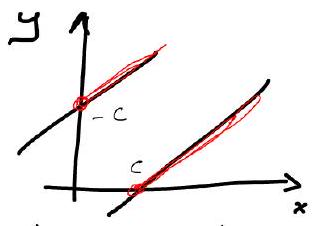
\includegraphics[width=\textwidth]{graphics/2025_10_17_109d3ce1ba98c27731a1g-3}
\end{figure}

\begin{DispWithArrows}[displaystyle, format=c]
\dot{x}=-k x(x-c)=k x(c-x)
\end{DispWithArrows}
This is called logistic equation and can be solved analytically:
\begin{DispWithArrows}[displaystyle, format=c]
x(t)=\frac{c x_{0} e^{c k t}}{c+x_{0}\left(e^{c k t}-1\right)}
\end{DispWithArrows}
\begin{figure}[H]
    \centering
    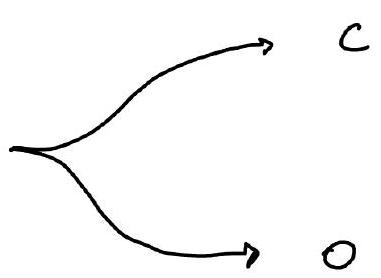
\includegraphics[width=0.5\textwidth]{graphics/2025_10_17_109d3ce1ba98c27731a1g-3(1)}
    \caption{if $c>0$ as $t \rightarrow+\infty$}
\end{figure}
if $c<0$

Check of (6) out. What happens if $c=0$? Solve eq. (4) for $z(t)$. There is
another independent conservation law: $\dot{x}+\dot{z}=0 \Rightarrow x(t)+z(t)=x_{0}+z_{0}$
Therefore if $c>0, z \longrightarrow x_{0}+z_{0}-c=z_{0}+y_{0}$ as $t \rightarrow \infty$;
all $y$ goes to $z$. If $c<0, z \rightarrow z_{0}+x_{0}$.

\begin{figure}[H]
    \centering
    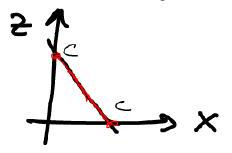
\includegraphics[width=\textwidth]{graphics/2025_10_17_109d3ce1ba98c27731a1g-3(2)}
\end{figure}

\subsection{Binary reversible reaction:}
\begin{DispWithArrows}[displaystyle, format=c]
x+y \underset{k_{-}}{\stackrel{k_{+}}{\rightleftarrows}} z \quad k_{ \pm}>0
\end{DispWithArrows}
Along the same lines as before we deduce the evolution of concent.
\begin{DispWithArrows}[displaystyle, format=l]
\left\{ \begin{aligned}
\dot{x} &=k_{-}z-k_{+}x y \\
\dot{y} &=k_{-}z-k_{+}x y \\
\dot{z} &=-k_{-}z+k_{+}x y
\end{aligned}\right.
\end{DispWithArrows}
Verify that there are two independent conservation laws $x(t)-y(t)=c_{1}$, and
$x(t)+z(t)=c_{2}$. Hence the eq. for $x$ can be written as
\begin{DispWithArrows}[displaystyle, format=c]
\dot{x}=k_{+} x\left(c_{1}-x\right)+k_{-}\left(c_{2}-x\right)
\end{DispWithArrows}
Obs: even this eq. can be solved analytically.

A more complicated case: the Haber process. This process was developed by F.
Haber in the early '900s for producing ammonia on an industrial scale: $N_{2}($
nitrogen $)+3 H_{2}($ hydrogen $) \longrightarrow 2 NH_{3}$ (ammonia) We
consider then the reaction:
\begin{DispWithArrows}[displaystyle, format=c]
X+3 Y \underset{k_{-}}{\stackrel{k_{+}}{\rightleftarrows}} 2 z
\end{DispWithArrows}
The ODEs for the concentrations are then:
\begin{DispWithArrows}[displaystyle, format=l]
\left\{\begin{aligned}
\dot{x} &=-k_{+} x y^{3}+k_{-} z^{2} \\
\dot{y} &=-3 k_{+} x y^{3}+3 k_{-} z^{2} \\
\dot{z} &=-2 k_{-} z^{2}+2 k_{+} x y^{3}
\end{aligned}\right.
\end{DispWithArrows}
The stoichiometric coefficients enter the ODEs:
Let's interpret the term $-3 k_{+} x y^{3}$ in eq. (11b)

Eq. (10) tells us that 3 molecules (or moles) of $Y$ have to collide
independently along with one molecule (or mole) of $X$ for the reaction to
occur in the forward (+) direction. Also, because for every molecule of $X$,
three molecules of $Y$ react, for a decrease in concentration of $x$, there is
a three fold decrease in concentration of $Y$. Thus, the stoichiometric
coefficients affect the prob. of a reaction to occur as well as the relative
speed of the reaction. Indeed, $3 \dot{x}=\dot{y}$, which relates the two
speeds of reaction.
The term $3 k_{-}z^{2}$ has a similar interpretation: for producing $Y$, two
molecules (moles) of $Z$ have to collide which will generate 3 molec. of $Y$.
Also, for every 2 molec. of $z$ that decompose in the backward direction
($k_{-}$), there will be 3 molec. of $Y$. This means that the speeds of
reaction are $3|\dot{z}|=2|\dot{y}|$. If we look at eq. 11.b,c we get
$3 \dot{z}=-2 \dot{y}$ because the decrease of $Y$ leads to an increase of $z$
and vice versa.

Obs: at stationarity $\frac{x y^{3}}{z^{2}}=\frac{k_{-}}{k_{+}}$, but there are
also some conservation laws:
\begin{DispWithArrows}[displaystyle, format=c]
3 x(t)-y(t)=c_{1}, \quad 2 x(t)+z(t)=c_{2}, \quad 2 y(t)+3 z(t)=c_{3}
\end{DispWithArrows}
Can you see why these quantities are conserved and why $c_{1}, c_{2}$ and
$c_{3}$ are not independent?

More generally, we can restate the law of mass action as

\subsection{The law of Mass Action}
In a first approximation, the rate of any chemical reaction is proportional to
the product of the concentration of the reacting substances, where every
concentration is raised to a power equal to the corresponding stoichiometric
coefficient which also has to be included in the reaction speed with the
appropriate sign.

Ex: write down the rate equation for the reversible reaction in eq.(1)
\begin{DispWithArrows}[displaystyle, format=c]
2 \mathrm{H}_{2}+\mathrm{O}_{2} \underset{k_{-}}{\stackrel{k_{t}}{\rightleftarrows}} 2 \mathrm{H}_{2} \mathrm{O}
\end{DispWithArrows}
The general reaction
\begin{DispWithArrows}[displaystyle, format=c]
a X+b Y \underset{k_{-}}{\stackrel{k_{+}}{\rightleftarrows}} c z+d W \quad a, b, c, d \in \mathbb{N}
\end{DispWithArrows}
leads to the following odes:
\begin{DispWithArrows}[displaystyle, format=l]
\left\{\begin{aligned}
\dot{x} &=a\left(-k_{+} x^{a} y^{b}+k_{-} z^{c} w^{d}\right) \\
\dot{y} &=b\left(-k_{+} x^{a} y^{b}+k_{-} z^{c} w^{d}\right) \\
\dot{z} &=c\left(+k_{+} x^{a} y^{b}-k_{-} z^{c} w^{d}\right) \\
\dot{w} &=d\left(+k_{+} x^{a} y^{b}-k_{-} z^{c} w^{d}\right)
\end{aligned}\right.
\end{DispWithArrows}
Calculate the quantities that are conserved.
There are types of molecules or species that can interact in different kinds of
reactions:
The predator $(Y)$ and prey $(X)$ system: (irreversible reactions)
\begin{DispWithArrows}[displaystyle, format=l]
\begin{aligned}
X & \xrightarrow{k_{1}} 2 X \\
Y+X & \xrightarrow{k_{2}} 2 Y \\
Y & \xrightarrow{k_{3}} \phi
\end{aligned}
\end{DispWithArrows}
reproduction of preys, predator eats a prey, predator dies.

To get the ODEs we have simply to sum the effects of different reactions:
\begin{DispWithArrows}[displaystyle, format=l]
\left\{\begin{aligned}
\dot{x} &=k_{1} x-k_{2} x y \\
\dot{y} &=k_{2} x y-k_{3} y
\end{aligned}\right.
\end{DispWithArrows}
These are the Lotka-Volterra equations. Show that at stationarity
$\bar{x}=\frac{k_{3}}{k_{2}}, \bar{y}=\frac{k_{1}}{k_{2}}$ but the Jacobian at
$(\bar{x}, \bar{y})$ has eigenvalues $\lambda= \pm i \sqrt{k_{1} k_{3}}$. Is the
system stable? Show that $V(x, y)=k_{2}(x+y)-k_{3} \ln x-k_{1} \ln y$ is a
conserved quantity.

\subsection{General chemical reactions}
More generally we may consider $m$ different chemical species $x_{i}, i=1, 2
\ldots m$ which are involved in $n$ different reactions of the form
\begin{DispWithArrows}[displaystyle, format=c]
\sum_{i=1}^{m} a_{i j} X_{i} \underset{k_{j}^{-}}{\stackrel{k_{j}^{+}}{\rightleftarrows}} \sum_{i=1}^{m} b_{i j} X_{i} \quad j=1, 2, \ldots, n
\end{DispWithArrows}
where $a_{i j}$ and $b_{i j}$ are stoichiometric coefficients that are all
non-negative integers.

Therefore the ODEs are
\begin{DispWithArrows}[displaystyle, format=c]
\dot{x}_{i}=\sum_{j=1}^{n}\left(b_{i j}-a_{i j}\right) r_{j}(\vec{x}) \quad i=1, 2, \ldots m
\end{DispWithArrows}
where $r_{j}(\bar{x}) \equiv k_{j}^{+} \prod_{i=1}^{m} x_{i}^{a_{i j}}-k_{j}^{-} \prod_{i=1}^{m} x_{i}^{b_{i j}} \quad$ for any $j=1, 2, \ldots, n$.
We want to find the conservation laws of eq. (16).
Let $S$ be the stoichiometric matrix: $S_{i j} \equiv b_{i j}-a_{i j}$ This is a
$m \times n$ matrix.
In vector form eq. (16) reads
\begin{DispWithArrows}[displaystyle, format=c]
\frac{d}{d t} \vec{x}=S \vec{r}(\vec{x})
\end{DispWithArrows}
A linear conserv. law for the system (15) or (16) has the form (if it exists)
\begin{DispWithArrows}[displaystyle, format=c]
\frac{d}{d t} \sum_{i=1}^{m} c_{i} x_{i}=0
\end{DispWithArrows}
where $c_{i}$ are (not all zero) constants. If $\sum_{i} c_{i} x_{i}(t)$ is a
constant of motion
\begin{DispWithArrows}[displaystyle, format=c]
\sum_{i} c_{i} x_{i}(t)=\sum_{i} c_{i} x_{i}(0)=\vec{c}^{\top} \cdot \vec{x}(0)
\end{DispWithArrows}
where $\vec{c}^{\top}=\left(c_{1}, c_{2}, \ldots, c_{m}\right)$. If we multiply
eq eq (17) by $\vec{c}^{\top}$, then
\begin{DispWithArrows}[displaystyle, format=c]
\vec{c}^{\top} \cdot \frac{d}{d t} \vec{x}=\vec{c}^{\top} S \vec{r}(\vec{x})=0
\end{DispWithArrows}
Eq. (19) holds true for all $\vec{r}$, hence it must be
\begin{DispWithArrows}[displaystyle, format=c]
\vec{c}^{\top} S=0 \quad \text { or } \quad S^{\top} \vec{c}=0
\end{DispWithArrows}
The conservation laws of the system of reactions in eq - (16) are given by the
non-zero elements $\vec{c} \in \operatorname{ker}\left(S^{\top}\right)$
($\vec{c}^{\top} \cdot \vec{x}=\text{const}$) and the number of (linearly
independent) conservation laws is given by
$\operatorname{dim}\left(\operatorname{ker}\left(s^{\top}\right)\right)$. For the
reaction 


Basis $(1,-1,0)$ and $(1,0,1) \rightarrow x-y=\text{const.}$
\begin{DispWithArrows}[displaystyle, format=c]
x+z=\text{ const. }
\end{DispWithArrows}
Tools for the simulation of chemical reactions
Many tools and libraries are available for the numerical simulation of chemical 
reactions:


It is good practice to write down your own code for you to check whether you
have understood the basics of the theory.

Also, these reactions should be implemented with stochastic algorithms which
account for the discrete nature of the particles. These tools will be provided
in the other part of the module.

% Lecture file created by newnote
% Class: Models of Theoretical Physics
% Professor: Azaele Sandro
% Date: 2025-10-17
\lecture{2}{Fokker-Planck equation}{2025-10-17}
\pagelayout{margin}
% --- Start writing here ---

\section{Fokker-Planck equation}
Derivation of the Fokker-Planck equation for a general Langevin equation (Itô prescription)

We start from a stochastic process defined via the Langevin equation (Itô)
\begin{DispWithArrows}[tag=1]
    d x(t)=\mu(x(t), t) d t+\sigma(x(t), t) d B(t)
\end{DispWithArrows}
where $x(0)=x_{0}$ (or a generic initial PDF). $B(t)$ is a standard Brownian process.
An alternative way to write eq. (1) is the "pseudo-equation"
\begin{DispWithArrows}[tag=2]
    \dot{x}=\mu(x, t)+\sigma(x, t) \xi(t)
\end{DispWithArrows}
Where $\langle\xi(t)\rangle=0$ and $\left\langle\xi\left(t^{\prime}\right) \xi(t)\right\rangle=\delta\left(t^{\prime}-t\right)$. We used the suggestive relation " $\frac{d B}{d t}=\xi$ ", even though this is only a formal, notational expression.

Eq. (1) defines the process $x(t)$ so we can use the eq. to generate as many trajectories as we wish. Let us assume that we have generated a large number $N$ of paths from time $t=0$ to $t=T>0$. How can we calculate the probability that $x(t)$ gets a value between $x$ and $x+\Delta x$ (a PDF) at time $t$?

From the computational point of view this is relatively easy:
\begin{figure}[H]
    \centering
    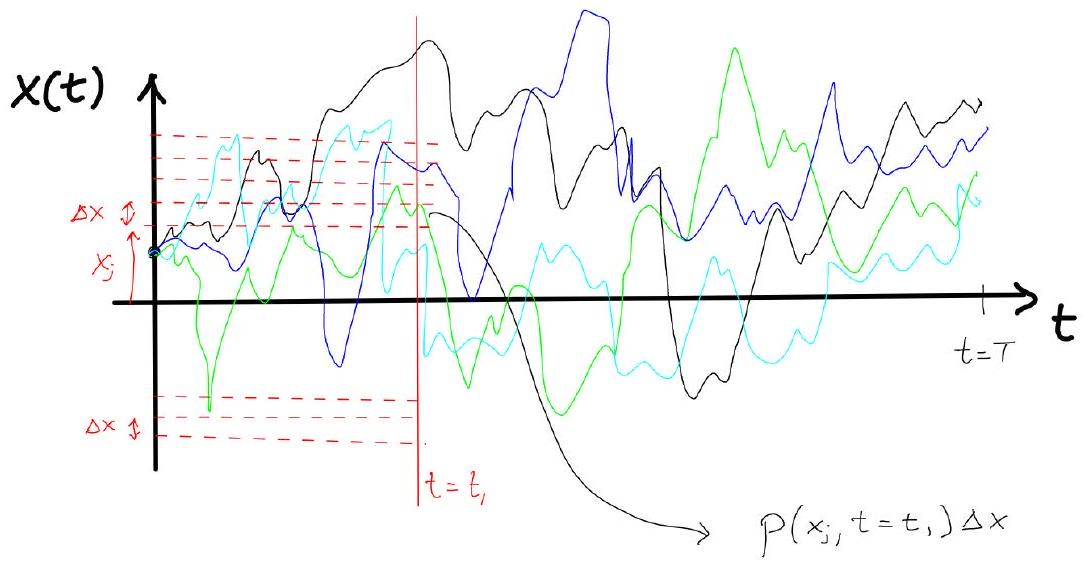
\includegraphics[width=0.8\textwidth]{2025_10_17_15d569b79a40ed74679eg-02}
\end{figure}
We have to count how many paths fall in the interval $[x, x+\Delta x)$ at time $t=t_{1}$ as $x$ varies in the domain of definition of the process $x(t)$.
If we use the indicator function, $I$, defined as
\begin{DispWithArrows}
    I(a, A)= \begin{cases}
    1 & a \in A \\
    0 & a \notin A
    \end{cases}
\end{DispWithArrows}
then we calculate numerically $P(x, t)$ as
\begin{DispWithArrows}[tag=3]
    P\left(x_{j}, t=t_{1}\right) \Delta x=\lim _{N \rightarrow \infty} \frac{1}{N} \sum_{1}^{N} I\left(x^{i}\left(t_{1}\right),\left[x_{j}, x_{j}+\Delta x\right)\right)
\end{DispWithArrows}
for any $x_{j}$ and various $t$.

Where $x_{j}=j \Delta x$ and $j=j_{\min }, j_{\min }+1, \ldots j_{\max }-1, j_{\max }$ (uniform mesh). For example, if the process was Brownian, then $P(x, t)$ would be very well approximated by a Gaussian distribution with zero mean and variance $t$, as we saw before. Notice that if we say $x_{j}=x, t=t$, and take the limit $\Delta x \rightarrow 0$, then
\begin{DispWithArrows}[tag=3b]
    P(x, t)=\lim _{N \rightarrow \infty} \frac{1}{N} \sum_{i}^{N} \delta\left(x-x_{i}(t)\right) \text { as } \lim _{\Delta x \rightarrow 0} \frac{I\left(x^{i}(t),[x, x+\Delta x)\right)}{\Delta x}=\delta\left(x-x_{i}(t)\right)
\end{DispWithArrows}
From the theoretical point of view we want to find out an equation for $P(x, t)$ which gives the PDF of the process $x(t)$. If we are interested in the statistics of the process, then $P(x, t)$ gives all the information we need, for we can calculate all averages we want (all moments) (even though it is not guaranteed that from the PDF we can exactly reconstruct the process $x(t)$ pathwise).
Actually, we can calculate the average of any "sufficiently regular" function $f$.
Let's assume that $f$ has compact support in $\mathbb{R}$ and is twice-differentiable, namely $f \in C_{c}^{2}(\mathbb{R})$.
Then we can calculate $\langle f(x(t))\rangle$, average of $f$ over the process. If we are given $N$ indep. realizations of $x(t)$, then as $N \rightarrow \infty$
\begin{DispWithArrows}
    $\langle f(x(t))\rangle=\lim _{N} \frac{1}{N} \sum_{i}^{N} f\left(x_{i}(t)\right)=\lim _{N} \frac{1}{N} \sum_{i}^{N} \int d x f(x) \delta\left(x-x_{i}(t)\right) = \int d x f(x) \lim _{N} \frac{1}{N} \sum_{i}^{N} \delta\left(x-x_{i}(t)\right) \stackrel{\downarrow}{=} \int d x f(x) p(x, t)$
\end{DispWithArrows}
Hence
\begin{DispWithArrows}[tag=5]
    $\frac{d}{d t}\langle f(x(t))\rangle \equiv \int \dot{p}(x, t) f(x) d x$
\end{DispWithArrows}
Here $\langle\cdots\rangle$ means that the average of $f$ has to be calculated over the whole set of trajectories of the process $x(t)$. We now discretize the process in time and Taylor-expand the function $f(x)$:
\begin{DispWithArrows}[tag=6]
    $f(x(t+\Delta t))=f(x(t))+\Delta x f^{\prime}(x(t))+\frac{\Delta x^{2}}{2} f^{\prime \prime}(x(t))+\text { h.o.t. }$
\end{DispWithArrows}
where from eq. (1) we get
\begin{DispWithArrows}[tag=7]
    $\Delta x \equiv x(t+\Delta t)-x(t)=\mu(x(t), t) \Delta t+\sigma(x(t), t) \Delta B(t)$
\end{DispWithArrows}
Therefore from (6) $\Delta f \equiv f(x(t+\Delta t))-f(x(t))$
\begin{DispWithArrows}
    \begin{aligned}
    \Delta f & =f^{\prime}(\mu \Delta t+\sigma \Delta B)+\frac{1}{2} f^{\prime \prime}(\mu \Delta t+\sigma \Delta B)^{2}+\text { h.o.t. } \\
    & =f^{\prime}(\mu \Delta t+\sigma \Delta B)+\frac{1}{2} f^{\prime \prime}\left(\mu^2\Delta t^2 + 2 \mu \sigma \Delta t \Delta B+\sigma^{2} \Delta B^{2}\right)+\text { h.o.t. }
    \end{aligned}
\end{DispWithArrows}
We now consider the average of each term:
a) $\left\langle f^{\prime} \sigma \Delta B\right\rangle=\left\langle f^{\prime} \sigma\right\rangle\langle\Delta B\rangle=0$ (Itô prescription)
b) $\left\langle f^{\prime \prime} \mu \sigma \Delta t \Delta B\right\rangle=\left\langle f^{\prime \prime} \mu \sigma\right\rangle \Delta t\langle\Delta B\rangle=0$
c) $\frac{1}{2}\left\langle f^{\prime \prime} \sigma^{2} \Delta B^{2}\right\rangle=\frac{1}{2}\left\langle f^{\prime \prime} \sigma^{2}\right\rangle\left\langle\Delta B^{2}\right\rangle=\frac{1}{2}\left\langle f^{\prime \prime} \sigma^{2}\right\rangle \Delta t$ (Itô preser. IMPORTANT!)
all remaining terms are $O\left(\Delta t^{2}\right)$.
Therefore eq. (5) can be re-written as limit
\begin{DispWithArrows}[tag=9]
    \lim _{\Delta t \rightarrow 0}\left\langle\frac{\Delta f}{\Delta t}\right\rangle=\left\langle f^{\prime} \mu\right\rangle+\frac{1}{2}\left\langle f^{\prime \prime} \sigma^{2}\right\rangle = \int d x p(x, t)\left[f^{\prime}(x) \mu(x, t)+\frac{1}{2} f^{\prime \prime}(x) \sigma^{2}(x, t)\right]
\end{DispWithArrows}
As $f \in C_{c}^{2}(\mathbb{R})$ we can integrate by parts and safely assume that $f, f^{\prime}$ and $f^{\prime \prime} \rightarrow 0$ as $|x|$ is large enough. Hence
\begin{DispWithArrows}[tag=10]
    $\int d x p(x, t) \mu(x, t) \frac{\partial f}{\partial x} \stackrel{\downarrow}{=}-\int d x f(x) \frac{\partial}{\partial x}(p \mu)$
\end{DispWithArrows}
twice integrated by parts
\begin{DispWithArrows}
    $\int d x p(x, t) \frac{\sigma^{2}(x, t)}{2} \frac{\partial^{2} f}{\partial x^{2}}=\frac{1}{2} \int d x f(x) \frac{\partial^{2}}{\partial x^{2}}\left(\sigma^{2}(x) p\right)$
\end{DispWithArrows}
and
\begin{DispWithArrows}
    $\frac{d}{d t}\langle f(x)\rangle=\int d x f(x) \frac{\partial}{\partial t} p(x, t)$
\end{DispWithArrows}
Thus from eqs. (9) and (10) and because $f \in C_{c}^{2}(\mathbb{R})$ but arbitrary we end up with
\begin{DispWithArrows}[tag=11]
    $\frac{\partial}{\partial t} p(x, t)=-\frac{\partial}{\partial x}[\mu(x, t) p(x, t)]+\frac{1}{2} \frac{\partial^{2}}{\partial x^{2}}\left[\sigma^{2}(x, t) p(x, t)\right]$
\end{DispWithArrows}
This is the forward Fokker-Planck equation corresponding to the process defined in eq. (1) with the Itô prescription. The FP eq. (11) can be used to derive the propagator of the process $x(t)$; we need just to solve it with the initial condition $P\left(x, t_{0}\right)=\delta\left(x-x_{0}\right)$, namely, this gives the fundamental solution $P\left(x, t \mid x_{0}, t_{0}\right)$. If we can calculate $P(x, t)$ then we can find all the averages (= statistics) of the process defined by the Langevin eq. (1). Notice that eq. (11) is a deterministic and linear PDE for $p(x, t)$.

Eq. (11) can also be written as
\begin{DispWithArrows}
    $\frac{\partial p}{\partial t}=-\frac{\partial J}{\partial x}(x, t)$
\end{DispWithArrows}
\begin{DispWithArrows}[tag=12]
    $J(x, t) \equiv \mu(x, t) p(x, t)-\frac{1}{2} \frac{\partial}{\partial x} \sigma(x, t) p(x, t)$
\end{DispWithArrows}
where $J(x, t)$ is the flux at $x$ at time $t$. This form shows that, if the process $x(t)$ is defined in the domain $D \subseteq \mathbb{R}$, then
\begin{DispWithArrows}
    $\frac{\partial}{\partial t} \int_{D} p(x, t) d x=-\int_{D} \frac{\partial J}{\partial x} d x=-\left.J\right|_{x \in \partial D}$
\end{DispWithArrows}
where $\partial D$ is the boundary of $D$. If there is no "leakage" of probability, then $\left.J\right|_{x \in \partial D}=0$ and we can set $\int_{D} p(x, t) d x=1$ at any time $t$ (conservation of probability).

Notice that eq. (11) must be equipped with boundary conditions if the process $x(t)$ is defined in given domain $D \subset \mathbb{R}$. For instance, if $D=\mathbb{R}^{+}$one has to define what happens at $x=0$ at any time $t>0$.

    * Absorbing boundary conditions require: $\left.p(x, t)\right|_{x \in \partial D}=0, \forall t$
    * Reflecting boundary conditions require: $\left.J(x, t)\right|_{x \in \partial D}=0 \quad \forall t$ N.B: these are the correct conditions when $\left.\sigma(x, t)\right|_{x \in \partial D}>0 \quad \forall t$

\subsection*{Equilibrium solution of the Fokker-Planck equation}
Let us assume that $\mu(x, t)=\mu(x)$ and $\sigma(x, t)=\sigma(x)$ and also that the propagator defined by eq. (11) reaches an equilibrium solution, namely
\begin{DispWithArrows}
    $\lim _{t \rightarrow \infty} p\left(x, t \mid x_{0}, t_{0}\right)=p^{s t}(x)$
\end{DispWithArrows}
what is the form of $p^{s t}(x)$? From. eq. (11) $\partial_{t} p^{s t}=0$ implies
\begin{DispWithArrows}
    $-\frac{\partial}{\partial x}\left(\mu(x) p^{s t}-\frac{1}{2} \frac{\partial}{\partial x} \sigma^{2}(x) p^{s t}\right)=0$
\end{DispWithArrows}
hence
\begin{DispWithArrows}
    $J^{s t}(x)=\mu(x) p^{s t}-\frac{1}{2} \frac{\partial}{\partial x} \sigma^{2}(x) p^{s t}=\text { const } \text { for any } x \text { . }$
\end{DispWithArrows}
If there is no current at any point $x \in D$, we obtain the equilibrium solution (with reflecting boundary conditions at $\partial D$)
\begin{DispWithArrows}
    $\mu(x) p^{s t}(x)=\frac{1}{2} \frac{\partial}{\partial x}\left(\sigma^{2}(x) p^{s t}(x)\right)$
\end{DispWithArrows}
Since
\begin{DispWithArrows}
    \begin{aligned}
    & \frac{2 \mu}{\sigma^{2}}\left(\sigma^{2} p^{s t}\right)=\frac{\partial}{\partial x}\left(\sigma^{2} p^{s t}\right) \\
    & \sigma^{2} p^{s t}=\text { const } e^{\int^{x} \frac{2 \mu}{\sigma^{2}} d y}
    \end{aligned}
\end{DispWithArrows}
hence the equilibrium solution has the form (ref.bound. at $x_{m}, x_{M}$)
\begin{DispWithArrows}[tag=13]
    $p^{s t}(x)=\frac{1}{Z} \frac{1}{\sigma^{2}(x)} e^{2 \int_{x_{m}}^{x} \frac{\mu(y)}{\sigma^{2}(y)} d y} \quad x_{m} \leq x \leq x_{M}$
\end{DispWithArrows}
where $Z \equiv \int_{x_{m}}^{x_{M}} \frac{d x}{\sigma^{2}(x)} e^{2 \int_{x_{m}}^{x} \frac{\mu(y)}{\sigma^{2}(y)} d y}<\infty$, and $\int_{x_{m}}^{x_{M}} p^{s t}(x) d x=1$.
Some caveats:
Notice that eq. (13) may not exist. Also we have not proved that it is unique, nor that it can be reached by some initial conditions.
Eq. (13) is only the form one expects if indeed an equilibrium solution exists. Indeed, it does not depend on initial conditions and the equilibrium sol. is only determined by $\mu$ and $\sigma$ (and the ref.b.c.), so it is an intrinsic property of the system which is not tuned by how we initially prepare the system.

\subsection*{The Ornstein-Uhlenbeck process}
As a simple application of what we have studied we investigate the O.-U. process. From previous lectures we know that it is defined by the SDE
\begin{DispWithArrows}[tag=14]
    \left\{\begin{array}{lll}d x=-\mu x d t+\sigma d B(t) & \text { or } & \dot{x}=-\mu x+\sigma \xi_{t} \\ x(0)=x_{0} & \left(\left\langle\xi_{t}\right\rangle=0,\left\langle\xi_{t} \xi_{t^{\prime}}\right\rangle=\delta\left(t-t^{\prime}\right)\right)\end{array}\right.
\end{DispWithArrows}
Where $\mu, \sigma$ are positive constants and $B$ is the B.m. From e. (11) we obtain the F.P. equation for the PDF:
\begin{DispWithArrows}[tag=15]
    $\dot{p}=-\frac{\partial}{\partial x}[(-\mu x) p]+\frac{\sigma^{2}}{2} \frac{\partial^{2}}{\partial x^{2}} p$
\end{DispWithArrows}
The equilibrium distribution of (15) (from eq. (13)) is
\begin{DispWithArrows}
    $p^{s t}(x) \propto e^{-\frac{2}{\sigma^{2}} \int^{x} \mu y d y}=e^{-\frac{\mu}{\sigma^{2}} x^{2}}$
\end{DispWithArrows}
\begin{DispWithArrows}[tag=16]
    $p^{s t}(x)=\sqrt{\frac{\mu}{\pi \sigma^{2}}} e^{-\frac{\mu}{\sigma^{2}} x^{2}}$
\end{DispWithArrows}
which is a Gaussian distribution with mean 0 and variance $\frac{\sigma^{2}}{2 \mu}$.
Exercise: Show that the equation for the variance that one gets from eq. (14) is the same that one gets from eq. (15). Verify that at stationarity the value is $\sigma^{2} / 2 \mu$.

Indeed one can calculate the evolution in time of the PDF.

By taking the Fourier transform of eq. (15) (which gives you the time evolution of the characteristic function of the process) one finds the full solution (which is the propagator of the O.-U. process)
\begin{DispWithArrows}[tag=17]
    $p\left(x, t \mid x_{0}, s\right)=\sqrt{\frac{\mu}{\pi \sigma^{2}\left(1-e^{-\mu(t-s)}\right)}} e^{-\frac{\mu}{\sigma^{2}} \frac{\left(x-x_{0} e^{-\mu(t-s)}
ight)^{2}}{1-e^{-\mu(t-s)}}}$
\end{DispWithArrows}
for which $P\left(x, s \mid x_{0}, s\right)=\delta\left(x-x_{0}\right)$. Another way to find the solution is to start from the ansatz
\begin{DispWithArrows}
    $p(x, t) \propto e^{-A x^{2}+x B+C}$
\end{DispWithArrows}
sub this into eq. (15) and find $A, B$ and $C$ as a function of $t$ and $x_{0}$. The normalization and the initial condition finally give eq.(17).

All these findings can be generalized to the case
\begin{DispWithArrows}
    $\dot{p}=-\frac{\partial}{\partial x}[(\alpha-\mu x) p]+\frac{\sigma^{2}}{2} \frac{\partial^{2}}{\partial x^{2}} p$
\end{DispWithArrows}
and also to the multidimensional O.-U. process (Gardiner, p. 105).

\subsection*{Particle in a large medium}
We study the motion of a particle suspended in a large (fluid) medium. The particle should be much bigger than those of the medium but small enough to change position and momentum when colliding with the medium's particles. The surrounding medium is a heat bath at thermal equilibrium with a const. temperature $T$ (homogeneous and isotropic).
If we had to account for all interactions of the suspended (mesoscopic) particle of mass $m$, we would write
\begin{figure}[H]
    \centering
    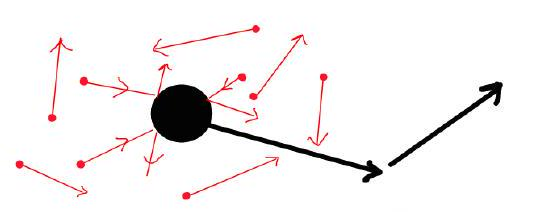
\includegraphics[width=0.5\textwidth]{2025_10_17_15d569b79a40ed74679eg-10}
\end{figure}
    * Fluid particles at temp T
    * mesoscopic particle
\begin{DispWithArrows}[tag=18]
    $m \ddot{\vec{x}}(t)=\vec{F}_{\text {ext }}(\vec{x}(t))+\sum_{i}^{N} i \vec{F}\left(\vec{x}(t)-\vec{x}_{i}(t)\right)$
\end{DispWithArrows}
where $\vec{F}_{\text {ext }}$ is an external force that may (or not) be described by a potential, where the i-th particle exerts on susp. particle a force $\bar{F}\left(\bar{x}-\overline{x_{i}}\right)$. As $N \simeq N_{A}$ (Avogadro number), it is pointless to integrate eq. (18). It's more appropriate to treat the medium particles in an effective way, like an effective force acting on the susp. particle. Thus
\begin{DispWithArrows}
    $\sum_{i}^{N} i \vec{F}\left(\vec{x}(t)-\vec{x}_{i}(t)\right) \simeq \vec{F}_{\text {aver }}+\vec{F}_{\text {noise }}$
\end{DispWithArrows}
As the mesoscopic particle collides with the smaller fluid particles there is viscous damping generated by the collisions in the fluid. If the velocity of the particle isn't too large we can approximate $\vec{F}_{\text {aver }}=-\gamma \vec{v}=-\gamma \dot{\vec{x}}, \gamma$ being the damping coefficient. From hydrodynamics, we can set $\gamma=6 \pi \eta R$, $\eta$ being the viscosity and $R$ the Brownian particle's radius.
We also assume that all fluid particles have independent motions and every particle's movement is independent on different time intervals (if not too small).

Also, if there is a time interval $\tau$ (much smaller of time intervals of observation $\Delta t$) large enough that in any two successive time intervals $\tau$ the motions of the mesoscopic particle can be considered independent events, then we can effectively approximate $\vec{F}_{\text {noise }}$ as a stochastic process that is proportional to a Brownian motion.
For simplicity, let's consider the 1-d case with no external forces. So from (18)
\begin{DispWithArrows}[tag=19]
    $m \ddot{x}=-\gamma \dot{x}+\sigma \xi(t)$
\end{DispWithArrows}
where $\langle\xi\rangle=0$ and $\left\langle\xi(t) \xi\left(t^{\prime}\right)\right\rangle=\delta\left(t-t^{\prime}\right)$. Notice that this process is non-Markovian. Let's multiply both sides by $x$, then
\begin{DispWithArrows}
    $m x \frac{d}{d t} \dot{x}=-\gamma x \dot{x}+\sigma x \xi_{t}$
\end{DispWithArrows}
Since $\frac{d^{2}}{d t^{2}} x^{2}=2\left(\dot{x}^{2}+x \ddot{x}\right)$, then
\begin{DispWithArrows}
    $\frac{m}{2} \frac{d^{2}}{d t^{2}}\left(x^{2}\right)-m \dot{x}^{2}=-\frac{\gamma}{2} \frac{d}{d t}\left(x^{2}\right)+\sigma x \xi_{t}$
\end{DispWithArrows}
Take the average of both sides and use Itô prescription:
\begin{DispWithArrows}
    $\frac{m}{2} \frac{d^{2}}{d t^{2}}\left\langle x^{2}\right\rangle-m\left\langle\dot{x}^{2}\right\rangle=-\frac{\gamma}{2} \frac{d}{d t}\left\langle x^{2}\right\rangle$
\end{DispWithArrows}
Because of the equipartition theorem in classical mechanics
\begin{DispWithArrows}
    $\frac{m}{2}\left\langle\dot{x}^{2}\right\rangle=\frac{1}{2} k_{B} T$
\end{DispWithArrows}
$k_{B}$ : Boltzmann's constant
hence T: absolute temperature
\begin{DispWithArrows}[tag=19b]
    $m \frac{d^{2}}{d t^{2}}\left\langle x^{2}\right\rangle+\gamma \frac{d}{d t}\left\langle x^{2}\right\rangle=2 k_{B} T$
\end{DispWithArrows}
Define $y(t)=\frac{d}{d t}\left\langle x^{2}\right\rangle$, then (19b) becomes
\begin{DispWithArrows}
    $m \dot{y}+\gamma y=2 k_{B} T$
\end{DispWithArrows}
Whose solution is $y(t)=c e^{-\frac{\gamma}{m} t}+\frac{2 k_{B} T}{\gamma}$ and $c$ is an arbitrary constant.
In suspended particles $\frac{m}{\gamma} \simeq 10^{-8} \mathrm{sec}$, which on temporal scales of observation is a tiny time. Hence for $t \gg 10^{-8} \mathrm{sec}, y \simeq \frac{2 k_{B} T}{\gamma}$ and
\begin{DispWithArrows}
    $\frac{d}{d t}\left\langle x^{2}\right\rangle \simeq \frac{2 k_{B} T}{\gamma}$
\end{DispWithArrows}
so
\begin{DispWithArrows}[tag=20]
    $\left\langle x^{2}(t)\right\rangle-\left\langle x_{0}^{2}\right\rangle=\frac{2 k_{B} T}{\gamma} t \text { for } t \gg 10^{-8} \mathrm{sec}$
\end{DispWithArrows}
linear increase of the mean square deviation.
This reminds us of the simple Brownian motion. Indeed, let's start from
\begin{DispWithArrows}[tag=21]
    $\dot{x}=\sqrt{2 D} \xi_{t} \text { or } d x=\sqrt{2 D} d B(t)$
\end{DispWithArrows}
which leads to the diffusive equation
\begin{DispWithArrows}
    $\frac{\partial}{\partial t} p(x, t)=D \frac{\partial^{2}}{\partial x^{2}} p(x, t) \quad D \text { is diffusivity }$
\end{DispWithArrows}
From (21) $x(t)=x_{0}+\sqrt{2 D} B(t)$ and
\begin{DispWithArrows}[tag=22]
    $\left\langle x^{2}\right\rangle=\left\langle x_{0}^{2}+2 x_{0} \sqrt{2 D} B(t)+2 D B(t)^{2}\right\rangle=x_{0}^{2}+2 D t$
\end{DispWithArrows}
diffusion law

By comparing eq. (20) and (22), we obtain
\begin{DispWithArrows}[tag=23]
    $D=\frac{k_{B} T}{\gamma}$
\end{DispWithArrows}
Einstein's relation

This is the first and simplest example of fluctuation-dissipation theorem.

\subsection*{Obs:}
    * Eq. (23) tells how we should choose the diffusivity if we want to interpret physically the mesoscopic particle as a free particle within an equilibrium thermal bath at temper. T.
    * $D$ does not depend on initial conditions, or the nature of interactions between the fluid particles and the Brownian particle, all we need to know is that the system is at equilibrium in a system where general behavior is summarized by the damping constant $\gamma$. (We captured some universal behavior here!).
    * From the diffusion law in eq. (22) one can measure $D$, hence we can give an estimate of $k_{B}$ and $N_{A}=\frac{R}{k_{B}}$, the Avogadro number ($R$ is the gas constant). This is what Einstein suggested in his 1905 pioneering work on Brownian motion.
    * This interpretation is straightforward if we start from eq. (19) with $\sigma=\sqrt{2 \gamma k_{B} T}$ and then take the limit $\frac{m}{\gamma} \rightarrow 0$ which is called the overdamped limit:
\begin{DispWithArrows}
    $\frac{m}{\gamma} \ddot{x}=-\dot{x}+\frac{\sqrt{2 \gamma k_{B} T}}{\gamma} \xi_{t} \xrightarrow{m / \gamma \rightarrow 0} \quad \dot{x}=\sqrt{2 \frac{k_{B} T}{\gamma}} \xi_{t}$
\end{DispWithArrows}
overdamped Langevin equation

\subsection*{Connection with Statistical Mechanics}
From stat. Mech. we know how to calculate the PDF that a particle has momentum $\vec{p}$ and position $\vec{x}$ when it is located within an external potential $U(\bar{x})$ and is surrounded by a heat bath at equilibrium at temperature $T$. This is
\begin{DispWithArrows}[tag=24]
    $\mathbb{P}(\vec{x}, \vec{p})=\frac{1}{z} e^{-\beta\left(\frac{\bar{p}^{2}}{2 m}+U(\bar{x})\right)} \quad \begin{gathered}\text { Boltzmann's weight } \\\beta=\frac{1}{k_{B} T}\end{gathered}$
\end{DispWithArrows}
where $m$ is the mass of the particle, $z=\int d \vec{p} \int d \vec{x} \mathbb{P}(\bar{x}, \bar{p})=\left(2 \pi m k_{B}\right)^{3 / 2} z_{0}$ is the total partition function and $z_{0}$ the reduced one. From eq. (24) one gets the PDF to observe the particle at $\vec{x}$ at equilibrium regardless of its momentum. This is
\begin{DispWithArrows}[tag=25]
    $w(\vec{x})=\frac{1}{z_{0}} e^{-\beta U(\vec{x})}$
\end{DispWithArrows}
Can we connect these classical results with the theory we have developed so far? Yes! We will do it for a 1-d system, but the generalization is simple and direct. Let's start from eq. (19) where now we assume that the particle experiences a conservative external force $f_{\text {ext }}=-\partial_{x} U(x)$, being $U(x)$ the potential of the force. We also assume that the Brownian particle is at equil. with the heat bath at temper. $T$, so $\sigma=\sqrt{2 \gamma k_{B} T}$:
\begin{DispWithArrows}[tag=26]
    $m \ddot{x}=-\partial_{x} U(x)-\gamma \dot{x}+\sqrt{2 \gamma k_{B} T} \xi_{t}$
\end{DispWithArrows}
In the overdamped limit ( $\frac{m}{\gamma} \rightarrow 0$ ) we get
\begin{DispWithArrows}[tag=27]
    $\dot{x}=-\frac{\partial_{x} U}{\gamma}+\sqrt{2 D} \xi_{t} \quad D=\frac{k_{B} T}{\gamma}$
\end{DispWithArrows}
or
\begin{DispWithArrows}
    $d x=-\frac{1}{\gamma} \partial_{x} U d t+\sqrt{2 D} d B(t)$
\end{DispWithArrows}
The corresponding Fokker-Planck equation of eq. (27) is
\begin{DispWithArrows}[tag=28]
    $\frac{\partial}{\partial t} p(x, t)=-\frac{\partial}{\partial x}\left[-\frac{1}{\gamma}\left(\partial_{x} U\right) p\right]+D \frac{\partial^{2}}{\partial x^{2}} p$
\end{DispWithArrows}
You can check that the equilibrium distribution of eq. (28) is given by (see eq. (13))
\begin{DispWithArrows}[tag=29]
    $P_{\text {eq }}(x) \propto e^{-\frac{1}{D \gamma} \int^{x} \partial_{y} U(y) d y} \propto e^{-\frac{1}{D \gamma} U(x)}$
\end{DispWithArrows}
but $D \gamma=k_{B} T$, so $P_{\text {eq }}(x)$ and $w(x)$ in eq. (25) are exactly the same.

\subsection*{Obs:}
    * Notice that we could have fixed $D=\frac{k_{B} T}{\gamma}$ by imposing that eq. (29) and (25) are the same! This is remarkable and shows that the value of $D$ does not depend on the potential $U$, which is somehow unexpected and confirms the universality of Einstein's relation in eq. (23).
    * Notice that if $U(x)=\frac{1}{2} k x^{2}$, then eq. (27) reads
\begin{DispWithArrows}
    $d x=-\frac{k}{\gamma} x d t+\sqrt{2 \frac{k_{B} T}{\gamma}} d B(t)$
\end{DispWithArrows}
\begin{figure}[H]
    \centering
    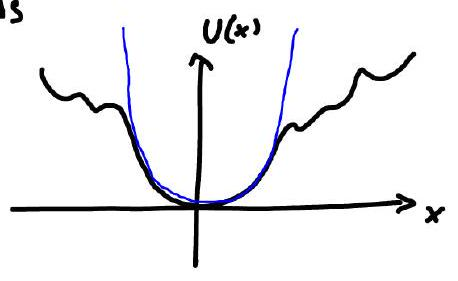
\includegraphics[width=\textwidth]{2025_10_17_15d569b79a40ed74679eg-15}
\end{figure}
which is an O.-U. process with the equilibrium distribution:
\begin{DispWithArrows}
    $p_{\text {eq }}(x)=\sqrt{\frac{k \beta}{2 \pi}} e^{-\frac{1}{2} \beta k x^{2}}$
\end{DispWithArrows}
Brownian particle in contact with a heat bath at equilibrium and forced by a harmonic potential. We start from eq. (26) where $U(x)=\frac{1}{2} k x^{2}$ and $\sigma=\sqrt{2 \gamma k_{B} T}$:
\begin{DispWithArrows}[tag=30]
    $m \ddot{x}=-k x-\gamma \dot{x}+\sqrt{2 \gamma k_{B} T} \xi_{t}$
\end{DispWithArrows}
where $x$ is the particle coordinate at time $t$, $m$ its mass, $\gamma$ the friction coefficient as before.
Eq. (30) is a linear eq. and can be solved even though the process is non-Markovian because of $\ddot{x}$. We write
\begin{DispWithArrows}
    $x(t)=x_{c}(t)+x_{\xi}(t)$
\end{DispWithArrows}
where $x_{c}$ satisfies the homogeneous eq.($\xi=0$) with $x_{c}(0)=x_{0}$ and $\dot{x}_{c}=v_{0}$. $x_{\xi}$ satisfies the in-homog. eq. with $x_{\xi}(0)=0$ and $\dot{x}_{\xi}(0)=0$.
Show that
\begin{DispWithArrows}
    $x_{c}(t)=A e^{-\gamma_{0} t} \sin (\Omega t)+B e^{-\gamma_{0} t} \cos (\Omega t)$
\end{DispWithArrows}
where $A, B$ are arbitrary constants and
\begin{DispWithArrows}
    $\gamma_{0}=\frac{\gamma}{2 m}, \quad \Omega=\omega_{0}^{2}-\gamma_{0}^{2}, \quad \omega_{0}^{2}=\frac{k}{m} ;
\end{DispWithArrows}
and
\begin{DispWithArrows}
    $x_{\xi}(t)=\sqrt{2 \gamma k_{B} T} \frac{1}{m \Omega} \int_{0}^{t} e^{-\gamma_{0}(t-s)} \sinh [\Omega(t-s)] \xi(s) d s$
\end{DispWithArrows}
Prove that
\begin{DispWithArrows}
    $\left\langle x^{2}(t)\right\rangle=\frac{2 \gamma k_{B} T}{m^{2} \Omega^{2}} \int_{0}^{t} e^{-2 \gamma_{0}(t-s)} \sinh ^{2}[\Omega(t-s)] d s \underset{t \rightarrow \infty}{\longrightarrow} \frac{k_{B} T}{m \omega_{0}^{2}}$
\end{DispWithArrows}
    * Can you interpret this result from the physical point of view?
    * Repeat the calculations for the velocity $v(t)=\dot{x}$
    * Can you calculate $\langle x(t) x(s)\rangle$? If necessary, fix $|t-s|$ and take the limit $t \rightarrow \infty, s \rightarrow \infty$.

\section{Fokker-Planck equation derivation}
Derivation of the Folkee-Planck equation for a general Langevin equation (Itô prescription)

We start from a stochastic process defined vie the Langerin equation (Itô)
(1) $\quad d x(t)=\mu(x(t), t) d t+\sigma(x(t), t) d B(t)$
where $x(0)=x_{0}$ (or a generic initial $P D F$ ). $B(t)$ is a standard Brownion process.
An alternative way to write eq. (1) is the "psendo-equation"
(2) $\dot{x}=\mu(x, t)+\sigma(x, t) \xi(t)$

Where $\langle\xi(t)\rangle=0$ and $\left\langle\xi\left(t^{\prime}\right) \xi(t)\right\rangle=\delta\left(t^{\prime}-t\right)$. We used the sugfestive relation " $\frac{d B}{d t}=\xi$ ", even though this is only a formal, notational expression.

Eq. (1) defines the process $x(t)$ so we can use the ep. to generate as many trajectories as we wish. Let us assume that we have generated a lage number $N$ of poths from time $t=0$ to $t=T>0$. How con we colulate the probability that $x(t)$ gets a value between $x$ and $x+\Delta x$ (a PDF) at time $t$ ?

From the computational point of view this is relatively eosy :
\begin{center}
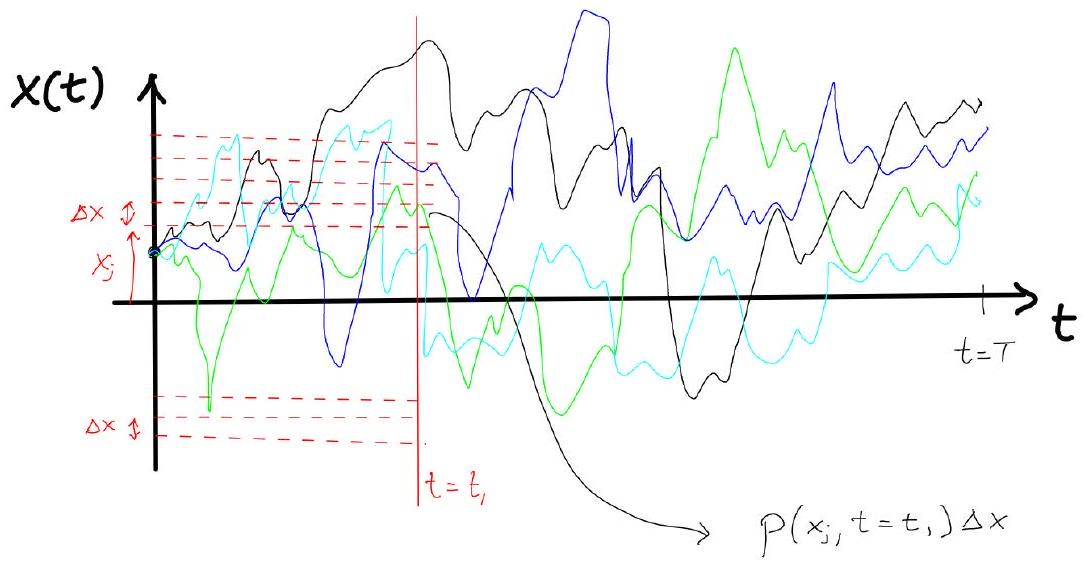
\includegraphics[width=\textwidth]{2025_10_17_1e406b49946272086d2dg-02}
\end{center}

$$
N=4
$$

We have to count how mony paths foll in the interval $[x, x+\Delta x)$ at time $t=t_{1}$ as $x$ veries in the domain of definition of the process $x(t)$.
If we use the indicator function, $I$, defined as

$$ I(a, A)= \begin{cases}1 & a \in A \ 0 & a \notin A\end{cases} $$

then we colculate numerically $P(x, t)$ as
(3) $P\left(x_{j}, t=t_{1}\right) \Delta x=\lim _{N \rightarrow \infty} \frac{1}{N} \sum_{1}^{N} I\left(x^{i}\left(t_{1}\right),\left[x_{j}, x_{j}+\Delta x\right)\right)$ for any $x_{j}$ and verious $t$.

Where $x_{j}=j \Delta x$ and $j=j_{\min }, j_{\min }+1, \ldots j_{\max }-1, j_{\max }$ (uniform mesh). For example, if the process was Brownion, then $P(x, t)$ would be very well approximated by a Gaussion distribution with zero mean and varience $t$, as we saw before. Notice that if we say $x_{j}=x, t=t$, and toke the limit $\Delta x \rightarrow 0$, then
(36) $P(x, t)=\lim _{N \rightarrow \infty} \frac{1}{N} \sum_{i}^{N} \delta\left(x-x_{i}(t)\right)$ es $\lim _{\Delta x \rightarrow 0} \frac{I\left(x^{i}(t),[x, x+\Delta x)\right)}{\Delta x}=\delta\left(x-x_{i}(t)\right)$

From the theoretical point of view we want to find out an equation for $P(x, t)$ which gives the PDF of the process $x(t)$. If we are interested in the statistics of the process, then $P(x, t)$ gives all the information we need, for we con
calculate all averages we wont (all moments)
(even though it is not guaranteed that from the PDF we con exactly reconstruct the process $x(t)$ pathwise).
Actually, we con calculate the average of any "sufficiently regular" function $f$.
Let's assume that $f$ has compact support in $\mathbb{R}$ and is twice-differentiable, mamely $f \in C_{c}^{2}(\mathbb{R})$.
Then we con calculate $\langle f(x(t))\rangle$, avarage of $f$ over the process. If we are given $N$ indep. zealizations of $x(t)$, then as $N \rightarrow \infty \langle f(x(t))\rangle=\lim _{N} \frac{1}{N} \sum_{i}^{N} f\left(x_{i}(t)\right)=\lim _{N} \frac{1}{N} \sum_{i}^{N} \int d x f(x) \delta\left(x-x_{i}(t)\right)=$


\begin{equation*}
=\int d x f(x) \lim _{N} \frac{1}{N} \sum_{i}^{N} \delta\left(x-x_{i}(t)\right) \stackrel{\downarrow}{=} \int d x f(x) p(x, t) \tag{35}
\end{equation*}


Hence

$$ \text { (5) } \quad \frac{d}{d t}\langle f(x(t))\rangle \equiv \int \dot{p}(x, t) f(x) d x $$

Here $\langle\cdots\rangle$ means that the average of $f$ has to be calculated over the whole set of trajectories of the process $x(t)$. We now diserentize the procen in time and Taylor-expand the function $f(x)$ :
(6) $f(x(t+\Delta t))=f(x(t))+\Delta x f^{\prime}(x(t))+\frac{\Delta x^{2}}{2} f^{\prime \prime}(x(t))+$ h.o.t.
where from ef. (1) we get
(7) $\quad \Delta x \equiv x(t+\Delta t)-x(t)=\mu(x(t), t) \Delta t+\sigma(x(t), t) \Delta B(t)$

Therefore from (6) $\Delta f \equiv f(x(t+\Delta t))-f(x(t))$

$$ \begin{aligned}
\Delta f & =f^{\prime}(\mu \Delta t+\sigma \Delta B)+\frac{1}{2} f^{\prime \prime}(\mu \Delta t+\sigma \Delta B)^{2}+\text { h.o.t. } \\
& =f^{\prime}(\mu \Delta t+\sigma \Delta B)+\frac{1}{2} f^{\prime \prime}\left(\mu^2\Delta t^2+2 \mu \sigma \Delta t \Delta B+\sigma^{2} \Delta B^{2}\right)+\text { h.o.t. }
\end{aligned} $$

We now consider the average of each term:
a) $\left\langle f^{\prime} \sigma \Delta B\right\rangle=\left\langle f^{\prime} \sigma\right\rangle\langle\Delta B\rangle=0$

Itô prescription
b) $\left\langle f^{\prime \prime} \mu \sigma \Delta t \Delta B\right\rangle=\left\langle f^{\prime \prime} \mu \sigma\right\rangle \Delta t\langle\Delta B\rangle=0$
c) $\frac{1}{2}\left\langle f^{\prime \prime} \sigma^{2} \Delta B^{2}\right\rangle=\frac{1}{2}\left\langle f^{\prime \prime} \sigma^{2}\right\rangle\left\langle\Delta B^{2}\right\rangle=\frac{1}{2}\left\langle f^{\prime \prime} \sigma^{2}\right\rangle \Delta t$ Itô preser. IMPORTANT!
all remaining terms are $O\left(\Delta t^{2}\right)$.
Therefore eq. (5) con be re-written as limit
(9) $\quad \lim _{\Delta t \rightarrow 0}\left\langle\frac{\Delta f}{\Delta t}\right\rangle=\left\langle f^{\prime} \mu\right\rangle+\frac{1}{2}\left\langle f^{\prime \prime} \sigma^{2}\right\rangle$

$$ =\int d x p(x, t)\left[f^{\prime}(x) \mu(x, t)+\frac{1}{2} f^{\prime \prime}(x) \sigma^{2}(x, t)\right] $$

As $f \in C_{c}^{2}(\mathbb{R})$ we can integrate by parts and safely assume that $f, f^{\prime}$ and $f^{\prime \prime} \rightarrow 0$ as $|x|$ is large enough. Hence
(10)

$$ \int d x p(x, t) \mu(x, t) \frac{\partial f}{\partial x} \stackrel{\downarrow}{=}-\int d x f(x) \frac{\partial}{\partial x}(p \mu) $$

twice integrated by parts

$$ \int d x p(x, t) \frac{\sigma^{2}(x, t)}{2} \frac{\partial^{2} f}{\partial x^{2}}=\frac{1}{2} \int d x f(x) \frac{\partial^{2}}{\partial x^{2}}\left(\sigma^{2}(x) p\right) $$

and

$$ \frac{d}{d t}\langle f(x)\rangle=\int d x f(x) \frac{\partial}{\partial t} p(x, t) $$

Thus from eps. (9) and (10) and because $f \in C_{c}^{2}(\mathbb{R})$ but arbitrary we end up with
(11) $\quad \frac{\partial}{\partial t} p(x, t)=-\frac{\partial}{\partial x}[\mu(x, t) p(x, t)]+\frac{1}{2} \frac{\partial^{2}}{\partial x^{2}}\left[\sigma^{2}(x, t) p(x, t)\right] $

This is the forward Fokker-Planck equation corresponding to the process defined in el. (1) with the Itop prescription. The FP ep. (11) con be used to derive the propagoton of the process $x(t)$; we need just to solve it with the imitial condition $P\left(x, t_{0}\right)=\delta\left(x-x_{0}\right)$, namely, this gives the fundamental solution $P\left(x, t \mid x_{0}, t_{0}\right)$. If we can colculate $P(x, t)$ then we can find all the averages (= statistics) of the procen defined by the Langevin ef. (1). Notice that ep. (11) is a deterministic and linear PDE for $p(x, t)$.

Eq. (11) can also be written as

$$ \frac{\partial p}{\partial t}=-\frac{\partial J}{\partial x}(x, t) $$

(12)

$$ J(x, t) \equiv \mu(x, t) p(x, t)-\frac{1}{2} \frac{\partial}{\partial x} \sigma(x, t) p(x, t) $$

where $J(x, t)$ is the flux at $x$ at time $t$. This form shows that, if the process $x(t)$ is defined in the domain $D \subseteq \mathbb{R}$, then

$$ \frac{\partial}{\partial t} \int_{D} p(x, t) d x=-\int_{D} \frac{\partial J}{\partial x} d x=-\left.J\right|_{x \in \partial D} $$

where $2 D$ is the boundary of $D$. If there is no "leakage" of probability, then $\left.J\right|_{x \in \partial D}=0$ and we con set $\int_{D} p(x, t) d x=1$ at any time $t$ (conservation of probability).

Notice that ep. (11) must be equipped with boundary conditions if the process $x(t)$ is defined in given domain $D \subset \mathbb{R}$. For instance, if $D=\mathbb{R}^{+}$one has to define what happens at $x=0$ at any time $t>0$.

\begin{itemize}
  \item Absorbing boundary conditions require: $\left.p(x, t)\right|_{x \in 20}=0, \forall t$
  \item Reflecting boundory conditions require: $\left.J(x, t)\right|_{x \in \partial D}=0 \quad \forall t$ N3: these are the correct conditions when $\left.\sigma(x, t)\right|_{x \in \partial D}>0 \quad \forall t$ Equilibrium solution of the Fokker-Planct equation Let us assume that $\mu(x, t)=\mu(x)$ and $\sigma(x, t)=\sigma(x)$ and also that the propogator defined by ef. (11) reaches an equilibrium solution, nancely
\end{itemize}

$$ \lim _{t \rightarrow \infty} p\left(x, t \mid x_{0}, t_{0}\right)=p^{s t}(x) $$

what is the form of $p^{s t}(x)$ ? From. ey. (11) $\partial_{t} p^{s t}=0$ implies

$$ -\frac{\partial}{\partial x}\left(\mu(x) p^{t}-\frac{1}{2} \frac{\partial}{\partial x} \sigma^{2}(x) p^{s t}\right)=0 $$

hence

$$ J^{s t}(x)=\mu(x) p^{s t}-\frac{1}{2} \frac{\partial}{\partial x} \sigma^{2}(x) p^{s t}=\text { const } \text { for any } x \text {. } $$

If there is no current at any point $x \in D$, we obtain the equilibrium solution (with reflecting boundory conditions at $\partial D$ )

$$ \mu(x) p^{s t}(x)=\frac{1}{2} \frac{\partial}{\partial x}\left(\sigma^{2}(x) p^{s t}(x)\right) $$

Since

$$ \begin{aligned}
& \frac{2 \mu}{\sigma^{2}}\left(\sigma^{2} p^{s t}\right)=\frac{\partial}{\partial x}\left(\sigma^{2} p^{s t}\right) \\
& \sigma^{2} p^{s t}=\text { const } e^{\int^{x} \frac{2 \mu}{\sigma^{2}} d y}
\end{aligned} $$

hence the equilibrium solution has the form (ref.bound. at $x_{m}, x_{m}$ )
(13)

$$ p^{s t}(x)=\frac{1}{2} \frac{1}{\sigma^{2}(x)} e^{2\int_{x_{m}}^{x} \frac{\mu(y)}{\sigma^{2}(y)} d y} \quad x_{m} \leq x \leq x_{\mu} $$

where $z \equiv \int_{x_{m}}^{x_{M}} \frac{d x}{\sigma^{2}(x)} e^{2 \int_{x_{m}}^{x} \frac{\mu(y)}{\sigma^{2}(y)} d y}<\infty$, and $\int_{x_{m}}^{x_{M}} p^{s t}(x) d x=1$.
Some caveats:
Notice that ep. (13) may not exist. Also we have not proved that it is unique, nor that it can be reached by some initial conditions.
Eq. (13) is only the form one expects if indeed an equilibrium solution exists. Indeed, it does not depend on initial conditions and the equilibrium sol. is only determined by $\mu$ and $\sigma$ (and the refe.b.c.), so it is an intrinsic property of the system which is not tuned by how we imitially prepare the system.

The Ornstein- Unleubeck proces
As a rimple application of what we have studied we investigate the O-U process. From previous lectures we know that it is defined by the SDE
(14) $\left\{\begin{array}{lll}d x=-\mu x d t+\sigma d B(t) & \text { or } & \dot{x}=-\mu x+\sigma \xi_{t} \\ x(0)=x_{0} & \left(\left\langle\xi_{t}\right\rangle=0,\left\langle\xi_{t} \xi_{t^{\prime}}\right\rangle=\delta\left(t-t^{\prime}\right)\right)\end{array}\right.$

Where $\mu, \sigma$ are positive constants and $B$ is the B.m. From e. II (I) we obtain the F.P. equation for the PDF:
(15) $\dot{p}=-\frac{\partial}{\partial x}[(-\mu x) p]+\frac{\sigma^{2}}{2} \frac{\partial^{2}}{\partial x^{2}} p$

The equilibrium distribution of (15) (from ep. (13)) is

$$ p^{s t}(x) \propto e^{-\frac{2}{\sigma^{2}} \int^{x} \mu y d y}=e^{-\frac{\mu}{\sigma^{2}} x^{2}} $$

(16)

$$ p^{s t}(x)=\sqrt{\frac{\mu}{\pi \sigma^{2}}} e^{-\frac{\mu}{\sigma^{2}} x^{2}} $$

which is a Gaussian distribution with mean 0 and variance $\frac{\sigma^{2}}{2 \mu}$.
Exercige: Show that the equation for the verionce that ane gets from ep. (14) is the some that one gets from ep. (15). Verify that at stationarity the value is $\sigma^{2} / 2 \mu$.

Indeed on con colculate the evolution in time of the PDF.

By taking the Fourier transform of ep. (15) (which gives you the time evolution of the characteristic function of the process) one finds the full solution (which is the propogetor of the $0 .-U$. pocess)
(17) $p\left(x, t \mid x_{0}, s\right)=\sqrt{\frac{\mu}{\pi \sigma^{2}\left(1-e^{-\mu(t-s)}\right)}} e^{-\frac{\mu}{\sigma^{2}} \frac{\left(x-x_{0} e^{-\mu(t-s)}\right)^{2}}{1-e^{-\mu(t-s)}}}$
for which $P\left(x, s \mid x_{0}, s\right)=\delta\left(x-x_{0}\right)$. Another way to find the solution is to stort from the ansots

$$ p(x, t) \propto e^{-A x^{2}+x B+C} $$

sub this into ey. (15) and find $A, B$ and $C$ as a function of $t$ and $x_{0}$. The normalization and the imitial condition finally give q.(17).

All these findings can be generalized to the case

$$ \dot{p}=-\frac{\partial}{\partial x}[(\alpha-\mu x) p]+\frac{\sigma^{2}}{2} \frac{\partial^{2}}{\partial x^{2}} p $$

and also to the multidimensional O.-U. procen (Gardiner, p. 105).

\section*{Porticle in a large medium}
We study the anotion of a particle suspended in a loye (fhid) medium. The particle should be much bigger than those of the medium but small enough to change position and momentum when calliding with the medium's particles. The surrounding medium is a heat bath at Hermal equilisrium with a const. temperoture $T$ (homgeneous and isotropic).
If we had to account fir all interactions of the suspended (mesoscopic) porticle of mass $m$, we would write
\begin{center}
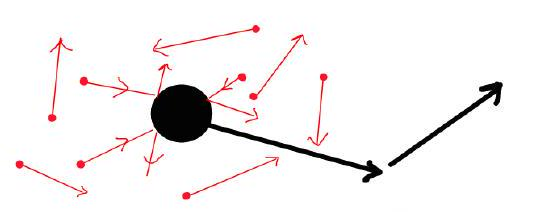
\includegraphics[width=0.5\textwidth]{2025_10_17_1e406b49946272086d2dg-10}
\end{center}

\begin{itemize}
  \item Lluid porticles at tem
  \item mesoscopic porticle
\end{itemize}


\begin{equation*}
m \ddot{\vec{x}}(t)=\vec{F}_{\text {ext }}(\vec{x}(t))+\sum_{i}^{N} i \vec{F}\left(\vec{x}(t)-\vec{x}_{i}(t)\right) \tag{18}
\end{equation*}


where $\vec{F}_{\text {ext }}$ is an external face that may (or not) be described by a potentiol, where the i-th porticle exerts on susp. particle e force $\bar{F}\left(\bar{x}-\overline{x_{i}}\right)$. As $N \simeq N_{A}$ (Avogadro number), it is pointlen to integrate ey. (18). It's more appropriate to treat the medium porticles in an effective way, like an effective force acting an the susp. porticle. Thus

$$ \sum_{i}^{N} i \vec{F}\left(\vec{x}(t)-\vec{x}_{i}(t)\right) \simeq \vec{F}_{\text {aven }}+\vec{F}_{\text {moise }} $$

As the mesoscopic particle callides with the smaller fluid partills there is viscons domping generated by the callisions in the fhid. If the velocity of the perticle isn't too lage we con approximate $\vec{F}_{\text {aver }}=-\gamma \vec{v}=-\gamma \dot{\vec{x}}, \gamma$ being the demping coefficient. From hydrodynomics, we con set $\gamma=6 \pi \eta R$, $\eta$ being the viscasity and $R$ the Browmion porticle's roolins.
We also assume that all fhid portilles have independent mestions and every porticle's movement is independent on different time intervals (if not too small).

Also, if there is a time interval $\tau$ (much smaller of time intervals of obsensation st) large enough that in any two successive time intends $r$ the motions of the mesosegric particle con be considered independent events, then we can effectivaly approximate $\vec{F}_{\text {moise }}$ as a stachastic process that is proportional to a Brownian motion.
For simplicity, let's consider the 1 -d cose with no extended forces. So from (18)


\begin{equation*}
m \ddot{x}=-\gamma \dot{x}+\sigma \xi(t) \tag{19}
\end{equation*}


where $\langle\xi\rangle=0$ and $\left\langle\xi(t) \xi\left(t^{\prime}\right)\right\rangle=\delta\left(t-t^{\prime}\right)$. Notice that this process is non-Morkovian. Let's multiply both sides by $x$, then

$$ m \times \frac{d}{d t} \dot{x}=-\gamma \times \dot{x}+\sigma \times \xi_{t} $$

Since $\frac{d^{2}}{d t^{2}} x^{2}=2\left(\dot{x}^{2}+x \ddot{x}\right)$, then

$$ \frac{m}{2} \frac{d^{2}}{d t^{2}}\left(x^{2}\right)-m \dot{x}^{2}=-\frac{\gamma}{2} \frac{d}{d t}\left(x^{2}\right)+6 x \xi_{t} $$

Take the average of both sides and use Iton presaiption:

$$ \frac{m}{2} \frac{d^{2}}{d t^{2}}\left\langle x^{2}\right\rangle-2 \cdot \frac{m}{2}\left\langle\dot{x}^{2}\right\rangle=-\frac{\gamma}{2} \frac{d}{d t}\left\langle x^{2}\right\rangle $$

Because of the equiportitien theorem in classical mechanics

$$ \frac{m}{2}\left\langle\dot{x}^{2}\right\rangle=\frac{1}{2} k_{B} T $$

$k_{B}$ : Boltz mom's constant
hence T: absolute temperature


\begin{equation*}
m \frac{d^{2}}{d t^{2}}\left\langle x^{2}\right\rangle+\gamma \frac{d}{d t}\left\langle x^{2}\right\rangle=2 k_{B} T \tag{196}
\end{equation*}


Define $y(t)=\frac{d}{d t}\left\langle x^{2}\right\rangle$, then (19b) becomes

$$ m \dot{y}+\gamma y=2 k_{B} T $$

Whose solution is $y(t)=c e^{-\frac{\gamma}{m} t}+\frac{2 k_{B} T}{\gamma}$ and $c$ is an arbitrary constant.
In suspended porticles $\frac{m}{\gamma} \simeq 10^{-8} \mathrm{sec}$, which on temporal scales of observation is a tiny time. Hence for $t \gg 10^{-8} \mathrm{sec}, y \simeq \frac{2 k B T}{\gamma}$ and

$$ \frac{d}{d t}\left\langle x^{2}\right\rangle \simeq \frac{2 k_{B} T}{\gamma} $$

so (20) $\left\langle x^{2}(t)\right\rangle-\left\langle x_{0}^{2}\right\rangle=\frac{2 k_{B} T}{\gamma} t$ for $t \gg 10^{-8} \mathrm{sec}$
limeas increase of the mean square deviation.
This seminds us of the simple Brownion motion. Indeed, let's stort from
(21) $\dot{x}=\sqrt{2 D} \xi_{t}$ or $d x=\sqrt{2 D} d B(t)$
which leads to the diffusive equation

$$ \frac{\partial}{\partial t} p(x, t)=D \frac{\partial^{2}}{\partial x^{2}} p(x, t) \quad D \text { is diffusivity } $$

From (21) $x(t)=x_{0}+\sqrt{2 D} B(t)$ and
(22)

$$ \left\langle x^{2}\right\rangle=\left\langle x_{0}^{2}+2 x_{0} \sqrt{2 D} B(t)+2 D B(t)^{2}\right\rangle=x_{0}^{2}+2 D t $$

diffusion law

By componing op. (20) and (22), we obtain
(23) $D=\frac{k_{B} T}{\gamma}$ Einstein's relation

This is the finst and simplest example of fluctuation-dissipation theorem.

\section*{Obs:}
\begin{enumerate}
  \item Eq. (23) tells how we should choose the diffusivity if we wont to interpret physically the menoscopic particle as a free perticle within an equilibrium therund both at temper. T.
  \item $D$ does not depend on initial conditions, or the nature of interactions between the fluid particles and the Brownion particle, all we need to know is that the system is at equilibrium in a system where general behaviou is summariged by the damping constant $\gamma$. (We coptured some universal behovion here!).
  \item From the diffusion law in ef. (22) one con measure $D$, hence We can give an estimete of $k_{B}$ and $N_{A}=\frac{R}{k_{B}}$, the Avogedro number ($R$ is the gas constant). This is what Einstein suggested in his 1905 pioneering wast on Brownian motion.
  \item This interputation is stroightforward if we start from ep. (19) with $\sigma=\sqrt{2 \gamma k_{B} T}$ and then take the limit $\frac{m}{\gamma} \rightarrow 0$ which is colled the overdomped limit:
\end{enumerate}

$$ \frac{m}{\gamma} \ddot{x}=-\dot{x}+\frac{\sqrt{2 \gamma k_{B} T}}{\gamma} \xi_{t} \xrightarrow{m / \gamma \rightarrow 0} \quad \dot{x}=\sqrt{2 \frac{k_{B} T}{\gamma}} \xi_{t} $$

overdomped Longevia equation
% !\TeX encoding = UTF-8
% Lecture file created by newnote
% Class: Models of Theoretical Physics
% Professor: Azaele Sandro
% Date: 2025-10-17
\lecture{4}{Turing Pattern Formation}{2025-10-17}
\pagelayout{margin}
% --- Start writing here ---

\section{Turing Pattern Formation}

Nature offers a wide range of examples of biological patterns, from animal
pigmentation to shells, skin, wings and skeletal structures. Patterns are
composed of spatially heterogeneous structures which may emerge owing to several
(biological) reasons. These could arise in systems in which chemicals react
with each other and also underwent diffusion - a mechanism which is termed
diffusion-driven instability. This is the basis of the so called Turing
patterns.
\begin{figure}[H]
  \centering
  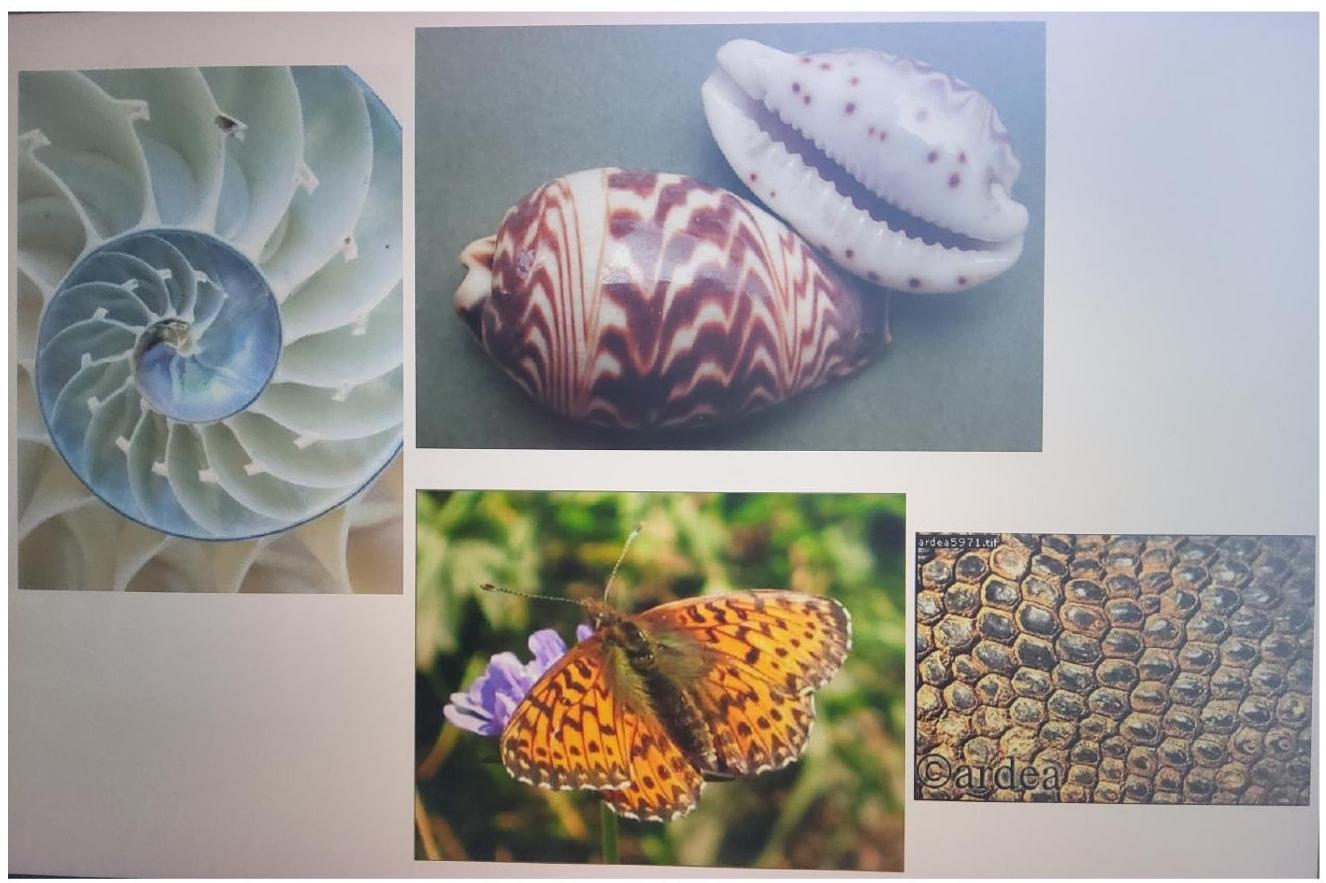
\includegraphics[width=\textwidth]{graphics/2025_10_17_3cf351a4349ae3691080g-01}
\end{figure}

Turing patterns and instability are related to symmetry breaking in
non-equilibrium systems and represent an example of emergent pattern, namely, a
structure that emerges from the combination of processes, which per se do not
possess any property related to the pattern itself.

In 1952 Alan Turing (logician, computer scientist, code breaker and
mathematician) proposed a mathematical model which was able to show emergent
patterns (A.M. Turing, the chemical basis of morphogenesis, Philos. Trans. R.
Soc. London B 237, 37-72, (1952)).

Turing showed that when some chemicals react with each other and diffuse
appropriately, then spatially heterogeneous patterns can emerge (diffusion-driven
instability), if some conditions are met.

\subsection*{One chemical species}
Let us consider the case with one chemical species, diffusing in a
one-dimensional space. We could consider the reactions
\begin{DispWithArrows}[displaystyle, format=l]
  \left.\begin{aligned}
      3 U &\underset{k_{-}}{\stackrel{k_{+}}{\rightleftarrows}} 2 U \      \phi &\underset{\mu_{-}}{\stackrel{\mu_{+}}{\rightleftarrows}} U
    \end{aligned}\right\} \rightarrow \dot{u}=-k_{+} u^{3}+k_{-} u^{2}-\mu_{-} u+\mu_{+1}
\end{DispWithArrows}
which involve only the species $U$ ($u$ is its concentration).
For the sake of generality, let's assume that the chemical $U$ is being produced
at rate $f(u)$ (typically a polynomial or a rational function of $u$). If we
include diffusion
\begin{DispWithArrows}[displaystyle, format=c]
  \frac{\partial u}{\partial t}=D \frac{\partial^{2} u}{\partial x^{2}}+f(u)
\end{DispWithArrows}
Where $D>0$ is the diffusion coefficient. Eq. (1) is a reaction-diffusion
equation.
We also assume that $U$ diffuses in a domain $(0,L)$ and that
\begin{DispWithArrows}[displaystyle, format=c]
  u(0, t)=u_{0}=u(L, t) \quad \forall t
\end{DispWithArrows}
These are called Dirichlet boundary conditions. If there is a spatially uniform
stationary state $u_0$ for $u$, then we also have
$\lim_{t \to \infty} u(x, t)=u_{0}$ and $f\left(u_{0}\right)=0$.
Is this state stable? In general this is a hard question, but we can check
whether $u_{0}$ is linearly stable. To check this we have to determine the
effect of a small perturbation.
$\hat{u}(x, t)=u(x, t)-u_{0} \quad\left(|\hat{u}| \ll u_{0}\right)$. Expanding
$f$ in a Taylor series we get (only linear terms) from eq. (1)
\begin{DispWithArrows}[displaystyle, format=c]
  \frac{\partial \hat{u}}{\partial t}=D \frac{\partial^{2} \hat{u}}{\partial x^{2}}+f^{\prime}\left(u_{0}\right) \hat{u} \quad \hat{u}(0, t)=0=\hat{u}(L, t)
\end{DispWithArrows}
where we assumed $f\left(u_{0}\right)=0$ and $f^{\prime}\left(u_{0}\right) \neq 0$.
Without space ($D=0$) we get
\begin{DispWithArrows}[displaystyle, format=c]
  \hat{u}(x, t)=\hat{u}_{0} e^{f^{\prime}\left(u_{0}\right) t}
\end{DispWithArrows}
$\hat{u}_{0}$ is the initial perturbation. Of course, the steady state is
stable if $f^{\prime}\left(u_{0}\right)<0$. If $D>0$, then eq. (3) can be solved
via separation of variables: $\hat{u}(x, t)=h(x) k(t)$. Thus we get from eq. (3)
\begin{DispWithArrows}[displaystyle, format=l]
  \begin{aligned}
    \left(\partial_{t} k\right) h & =D k\left(\partial_{x}^{2} h\right)+f^{\prime}\left(u_{0}\right) k h \    \frac{\partial_{t} k}{k} & =D \frac{\partial_{x}^{2} h}{h}+f^{\prime}\left(u_{0}\right)
  \end{aligned}
\end{DispWithArrows}
because the l.h.s. depends on $t$ only and the r.h.s. on $x$ only, it must be
\begin{DispWithArrows}[displaystyle, format=c]
  \underbrace{\frac{\partial_{t} k}{k}}_{a}=\lambda=\overbrace{D \frac{\partial_{x}^{2} h}{h}+f^{\prime}\left(u_{0}\right)}^{b}
\end{DispWithArrows}
Where $\lambda$ is constant independent of time and space
a) $\partial_{t} k=\lambda k \Rightarrow k(t)=k_{0} e^{\lambda t}$
b)
$\partial_{x x}^{2} h=\underbrace{\frac{\lambda-f^{\prime}\left(u_{0}\right)}{D}}_{-\rho^{2}} h \Rightarrow h(x)=A \sin (\rho x)+B \cos (\rho x)$

From the B.C. in eq. (2) we obtain $h(0)=0 \Rightarrow B=0$ and also
$h(L)=0 \Rightarrow \rho=\frac{n \pi}{L}$ for any $n=1,2 \ldots$
Hence the modes
\begin{DispWithArrows}[displaystyle, format=c]
  \lambda_{n}=f^{\prime}\left(u_{0}\right)-D\left(\frac{n \pi}{L}\right)^{2} \quad n=1,2, \cdots
\end{DispWithArrows}
Because the eq. is linear, we can sum all the modes and get the final solution
as a Fourier series:
\begin{DispWithArrows}[displaystyle, format=c]
  \hat{u}(x, t)=\sum_{n=1}^{\infty} a_{n} \sin \left(\frac{n \pi x}{L}\right) e^{\lambda_{n} t} \quad \hat{u}(0, t)=0=\hat{u}(L, t)
\end{DispWithArrows}
where $a_{n}$ are determined to satisfy the initial condition for the pert.
Note from (5) that, even if $f^{\prime}\left(u_{0}\right)>0$ ($u_{0}$ is
unstable), then $D>f^{\prime}\left(u_{0}\right)\left(\frac{L}{\pi}\right)^{2}$ (for
fixed domain size L) implies $\lambda_{n}<0$. Therefore, all terms in eq. (6)
with $a_{n} \neq 0$ have an expon. decay, hence $\hat{u} \rightarrow 0$ as
$t \rightarrow \infty$.
In this case the state $u_{0}$ is stabilized by diffusion, even when it is
unstable, if $D$ is sufficiently large. D cannot destabilize the solution.

\subsection{Exercise:}
If B.C. are zero-flux at the boundaries
$\left(\frac{\partial u}{\partial x}(0)=0=\frac{\partial u}{\partial x}(L)\right.$,
Neumann B.C.) the zeroth mode could still grow, but all the others decay
exponentially so there cannot be any spatial heterogeneity for large $D$. Same
arguments still hold for periodic B.C.

Obs: Notice that diffusivity is not always able to stabilize.
If we fix $D$ and increase $L$ when $f^{\prime}\left(u_{0}\right)>0$, then for
sufficiently large domain sizes
$\left(L>\sqrt{\frac{D \pi^{2}}{f^{\prime}\left(u_{0}\right)}}\right)$ we still get
$\lambda_{n}>0$. The effect of diffusion depends on the domain.

\subsection{Two or more chemical species}
From the previous section we have learnt that diffusion is able to smooth out
inhomogeneities, thus stabilizing processes. This agrees with other phenomena,
e.g., diffusion of heat within a finite domain.
Turing understood that if there are more than one interacting species, this is
not necessarily the case and diffusion may destabilize homogeneous solutions.
Let $u(x, t)$ and $v(x, t)$ be the concentrations of two chemical species which
satisfy the following reaction-diffusion equations in 1-d space:
\begin{DispWithArrows}[displaystyle, format=ll]
  \left.\begin{aligned}
      \dot{u}&=f(u, v)+D_{1} \frac{\partial^{2} u}{\partial x^{2}} \      \dot{v}&=g(u, v)+D_{2} \frac{\partial^{2} v}{\partial x^{2}}
    \end{aligned}\right\} \quad \text { with I.C. and B.C.}
\end{DispWithArrows}
where $f$ and $g$ are smooth functions which describe the reactions between the
two chemicals whose concentrations are given by $u$ and $v . D_{1}$ and $D_{2}$
are two diffusion constants. We assume that $x \in(0,L)$ (finite domain) and at
the boundaries we impose zero-flux conditions (Neumann b.c.).

Let us assume that eq. (7) admits a spatially uniform steady state, hence there
exist $u_{0}$ and $v_{0}$ such that
$f\left(u_{0}, v_{0}\right)=0=g\left(u_{0}, v_{0}\right)$. We now wish to derive
conditions of linear stability for the state $\left(u_{0}, v_{0}\right)$. For
this we introduce small (spatially-dependent) perturbations
$\hat{u}(x, t)=u(x, t)-u_{0}$ and $\hat{v}(x, t)=v(x, t)-v_{0}$ into eq. (7) and
expand $f$ and $g$ in Taylor series. We arrive at (recall that
$f\left(u_{0}, v_{0}\right)=0, g\left(u_{0}, v_{0}\right)=0$)
\begin{DispWithArrows}[displaystyle, format=l]
  \left.\begin{aligned}
      \dot{\hat{u}}&=\left.\frac{\partial f}{\partial u}\right|_{0} \hat{u}+\left.\frac{\partial f}{\partial v}\right|_{0} \hat{v}+D_{1} \frac{\partial^{2} \hat{u}}{\partial x^{2}} \      \dot{\hat{v}}&=\left.\frac{\partial g}{\partial u}\right|_{0} \hat{u}+\left.\frac{\partial g}{\partial v}\right|_{0} \hat{v}+D_{2} \frac{\partial^{2} \hat{v}}{\partial x^{2}}
    \end{aligned}\right.
\end{DispWithArrows}
where
$\left.\left.\frac{\partial f}{\partial u}\right|_{0} \equiv \frac{\partial f(u, v)}{\partial u}\right|_{\substack{u=u_{0} \ v=v_{0}}}$
and the same for the rest. We can recast eq. (8) in the matrix form
\begin{DispWithArrows}[displaystyle, format=c]
  \binom{\partial_{t} \hat{u}}{\partial_{t} \hat{v}}=\underbrace{\begin{pmatrix}
        \left.\frac{\partial f}{\partial u}\right|_{0} & \left.\frac{\partial f}{\partial v}\right|_{0} \        \left.\frac{\partial g}{\partial u}\right|_{0} & \frac{\partial g}{\left.\partial v\right|_{0}}
      \end{pmatrix}}_{\equiv J_{0}}\binom{\hat{u}}{\hat{v}}+\underbrace{\begin{pmatrix}
        D_{1} & 0 \        0 & D_{2}
      \end{pmatrix}}_{\equiv D}\binom{\partial_{x}^{2} \hat{u}}{\partial_{x}^{2} \hat{v}}
\end{DispWithArrows}
or
\begin{DispWithArrows}[displaystyle, format=c]
  \frac{\partial}{\partial t} \overrightarrow{\hat{u}}=J_{0} \overrightarrow{\hat{u}}+D \partial_{x}^{2} \overrightarrow{\hat{u}}
\end{DispWithArrows}
We carry out the analysis of the previous section and look for a solution of the
form
\begin{DispWithArrows}[displaystyle, format=c]
  \vec{u}(x, t)=\vec{a} e^{\left(i k x+\lambda\left(k^{2}\right) t\right)}
\end{DispWithArrows}
where $\vec{a}$ is a constant vector. Subbing (10) into (9) we get
\begin{DispWithArrows}[displaystyle, format=c]
  \lambda \vec{a} e^{i k x+\lambda t}=J_{0} \vec{a} e^{i k x+\lambda t}-k^{2} D \vec{a} e^{i k x+\lambda t}
\end{DispWithArrows}
which leads to the matrix equation
\begin{DispWithArrows}[displaystyle, format=c]
  \left(J_{0}-k^{2} D-\lambda \mathbb{1}\right) \vec{a}=\overrightarrow{0}
\end{DispWithArrows}
where $\mathbb{1}$ is the unit $2 \times 2$ matrix and
$\overrightarrow{0}=(0,0)^{T}$.

For non-trivial solutions to exist, we thus require that
\begin{DispWithArrows}[displaystyle, format=c]
  \operatorname{det}\left(J_{0}-k^{2} D-\lambda \mathbb{1}\right)=0
\end{DispWithArrows}
this condition provides us equations for obtaining the eigenvalues $\lambda$ (or
temporal growth rates) which are functions of $k^{2}$.
If we find $\operatorname{Re} \lambda>0$ for at least one eigenvalue then the
solution is unstable.

In the previous section we showed that an unstable fixed point can be
stabilized. Here we show that a stable homogeneous fixed point can be
destabilized by diffusion: this is the core of Turing pattern formation (and the
Turing's brilliant idea).
(1) A spatially-uniform steady state is linearly stable

Let us consider the case with no diffusion $D_{1}=D_{2}=0$.
Then $\lambda$ is the eigenvalue of the matrix $J_{0}$:
\begin{DispWithArrows}[displaystyle, format=c]
  \operatorname{det}\left(J_{0}-\lambda \mathbb{1}\right)=\operatorname{det}\begin{pmatrix}
    \partial_{u} f-\lambda & \partial_{v} f \    \partial_{u} g & \partial_{v} g-\lambda
  \end{pmatrix}=\left(\partial_{u} f-\lambda\right)\left(\partial_{v} g-\lambda\right)-\partial_{u} g \partial_{v} f=0
\end{DispWithArrows}
or
\begin{DispWithArrows}[displaystyle, format=c]
  \lambda^{2}-\underbrace{\left(\partial_{u} f+\partial_{v} g\right)}_{sum of sols} \lambda+\underbrace{\partial_{u} f \partial_{v} g-\partial_{v} f \partial_{u} g}_{prod. of sols. }=0
\end{DispWithArrows}
For the partially uniform steady state to be stable, both eigenvalues must have
negative real part, this leads to require that
\begin{DispWithArrows}[displaystyle, format=c]
  \partial_{u} f+\partial_{v} g<0 \quad \operatorname{Tr}\left(J_{0}\right)<0
\end{DispWithArrows}
\begin{DispWithArrows}[displaystyle, format=c]
  \partial_{u} f \partial_{v} g-\partial_{v} f \partial_{u} g>0 \quad \operatorname{Det}\left(J_{0}\right)>0
\end{DispWithArrows}
(2) A spatially-uniform steady state is linearly stable and is destabilized by
diffusion

When $D_{1}$ and $D_{2}$ are not zero, diffusion plays a role and changes the
eigenvalue problem. The determinant of eq. (12) leads to the equation
\begin{DispWithArrows}[displaystyle, format=c]
  \lambda^{2}-b\left(k^{2}\right) \lambda+c\left(k^{2}\right)=0
\end{DispWithArrows}
where
\begin{DispWithArrows}[displaystyle, format=ll]
  \begin{aligned}
    & b\left(k^{2}\right)=\partial_{u} f+\partial_{v} g-\left(D_{1}+D_{2}\right) k^{2} \    & c\left(k^{2}\right)=D_{1} D_{2} k^{4}-\left(D_{2} \partial_{u} f+D_{1} \partial_{v} g\right) k^{2}+\operatorname{det}\left(J_{0}\right)
  \end{aligned}
\end{DispWithArrows}
For diffusion to destabilize the fixed point a necessary condition is that at
least one of the roots of $\lambda\left(k^{2}\right)$ in eq. (16) has positive
real part for some non-zero (positive) $k^{2}$. This can happen if either $b>0$
or $c<0$. Now
\begin{DispWithArrows}[displaystyle, format=c]
  b=\partial_{u} f+\partial_{v} g \underbrace{-\left(D_{1}+D_{2}\right) k^{2}}_{\leqslant 0} \leqslant \partial_{u} f+\partial_{v} g<0 \quad \text {(from (14))}
\end{DispWithArrows}
So we must require $c\left(k^{2}\right)<0$. Now because
$\operatorname{det}(J_0)>0$ (from (15)), we must necessarily have
\begin{DispWithArrows}[displaystyle, format=c]
  D_{2} \partial_{u} f+D_{1} \partial_{v} g>0
\end{DispWithArrows}
Actually, this is a necessary, but not sufficient, condition for
$\operatorname{Re} \lambda>0$. For $c\left(k^{2}\right)$ to be negative for some
$k \neq 0$, the minimum of $c$ must be negative. The minimum of $c$ is (check
this!)
\begin{DispWithArrows}[displaystyle, format=c]
  C_{\text {min }}=\operatorname{det} J_{0}-\frac{\left(D_{2} \partial_{u} f+D_{1} \partial_{v} g\right)^{2}}{4 D_{1} D_{2}}
\end{DispWithArrows}
which is obtained when $k^{2}$ is
\begin{DispWithArrows}[displaystyle, format=c]
  k_{\text {min }}^{2}=\frac{D_{2} \partial_{u} f+D_{1} \partial_{v} g}{2 D_{1} D_{2}}
\end{DispWithArrows}
Thus the condition $c\left(k^{2}\right)<0$ requires $c_{\text {min }}<0$. From
(18)
\begin{DispWithArrows}[displaystyle, format=c]
  \frac{\left(D_{2} \partial_{u} f+D_{1} \partial_{v} g\right)^{2}}{4 D_{1} D_{2}}>\operatorname{det} J_{0}
\end{DispWithArrows}
which gives (= indicates a critical (bifurcation) value)
\begin{DispWithArrows}[displaystyle, format=c]
  D_{2} \partial_{u} f+D_{1} \partial_{v} g \geqslant 2 \sqrt{D_{1} D_{2}\operatorname{det} J_{0}}>0
\end{DispWithArrows}
\begin{figure}[H]
  \centering
  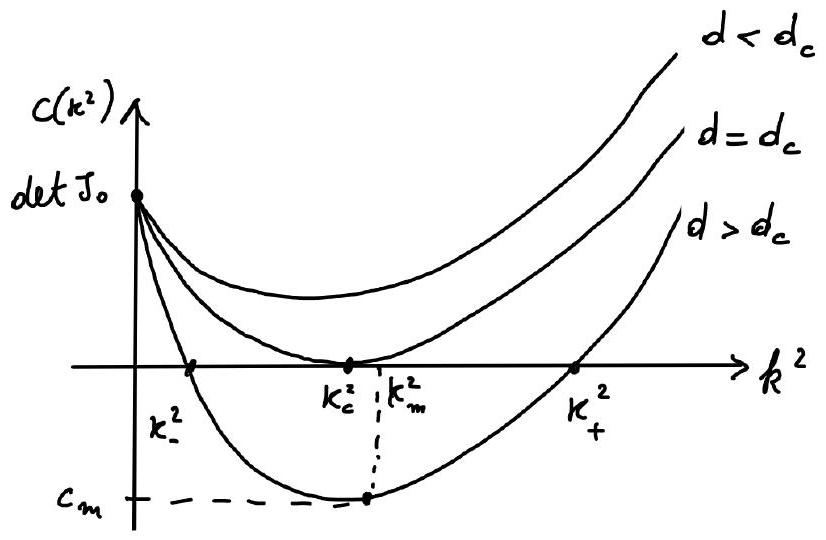
\includegraphics[width=0.5\textwidth]{graphics/2025_10_17_3cf351a4349ae3691080g-09}
  \caption{critical diffusivities ratio for Turing patterns to emerge.}
\end{figure}

\subsection*{Critical ratio ($d_c$)}
At the bifurcation $C_{\text {min }}=0$, which can be obtained only when $D_{1}$
and $D_{2}$ have a specific ratio. From eq. (20) and $\frac{D_{2}}{D_{1}}=d$ we
get
\begin{DispWithArrows}[displaystyle, format=c]
  \left(d \partial_{u} f+\partial_{v} g\right)^{2} \geqslant 4 d \operatorname{det} J_{0}>0
\end{DispWithArrows}
So the critical ratio $d_{c}$ of diffusivities satisfies the equation
\begin{DispWithArrows}[displaystyle, format=c]
  d_{c}^{2}\left(\partial_{u} f\right)^{2}+\left(\partial_{v} g\right)^{2}+2 d \partial_{u} f \partial_{v} g-4 d\left(\partial_{u} f \partial_{v} g-\partial_{v} f \partial_{u} g\right)=0
\end{DispWithArrows}
or
\begin{DispWithArrows}[displaystyle, format=c]
  d_{c}^{2}\left(\partial_{u} f\right)^{2}+2\left(2 \partial_{v} f \partial_{u} g-\partial_{u} f \partial_{v} g\right) d_{c}+\left(\partial_{v} g\right)^{2}=0
\end{DispWithArrows}
From $d_{c}$ we can calculate the critical wavenumber $k_{c}^{2}$. Indeed from
eq eq eq. (19)
\begin{DispWithArrows}[displaystyle, format=c]
  k_{\text {min }}^{2}=\frac{D_{2} \partial_{u} f+D_{1} \partial_{v} g}{2 D_{1} D_{2}}=\frac{1}{D_{1}} \frac{d \partial_{u} f+\partial_{v} g}{2 d}=\frac{1}{D_{1}} \sqrt{\frac{\operatorname{det}\left(J_{0}\right)}{d}}
\end{DispWithArrows}
from eq. (18) with $c_{\text {min }}=0$
from which we obtain (when $c_{\text {min }}=0, k_{\text {min }}=k_{c}$ ):
\begin{DispWithArrows}[displaystyle, format=c]
  k_{c}^{2}=\frac{1}{D_{1}} \sqrt{\frac{\operatorname{det}\left(J_{0}\right)}{d_{c}}}
\end{DispWithArrows}
where $d_{c}$ is from (21).

\subsection*{Conditions for Turing patterns to emerge}
Conditions (14), (15) and (20) ensure that the spatially uniform state is
linearly stable but has at least one wave number $k$ for which
$\lambda\left(k^{2}\right)$ has positive real part.
When we impose zero-flux boundary conditions, wavenumbers are restricted to
$k=\frac{n \pi}{L}$. Therefore there must exist at least one integer value
$n=1,2 \ldots$ for which $c\left(k^{2}\right)<0$ (in this case $d>d_{c}$). In
this case the range of unstable wavenumbers is obtained from the zeros
$k_{\pm}^{2}$ of $c\left(k^{2}\right)=0$ (see eq. (17)). We get
\begin{DispWithArrows}[displaystyle, format=c]
  k_{\pm}^{2}=\frac{D_{2} \partial_{u} f+D_{1} \partial_{v} g \pm \sqrt{\left(D_{2} \partial_{u} f+D_{1} \partial_{v} g\right)^{2}-4 D_{1} D_{2}\left(\partial_{u} f \partial_{v} g-\partial_{v} f \partial_{u} g\right)}}{2 D_{1} D_{2}}
\end{DispWithArrows}
\begin{DispWithArrows}[displaystyle, format=c]
  k_{-}^ {2} \leqslant\left(\frac{n \pi}{L}\right)^{2} \leqslant k_{+}^{2}
\end{DispWithArrows}
see also the previous figure and this one
\begin{figure}[H]
  \centering
  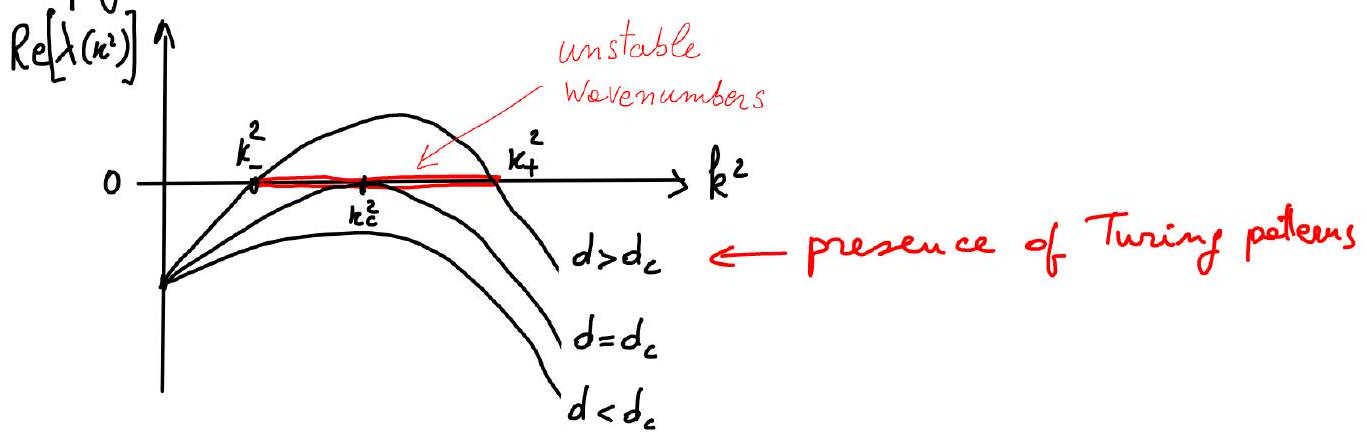
\includegraphics[width=0.5\textwidth]{graphics/2025_10_17_3cf351a4349ae3691080g-10}
\end{figure}

\subsection*{Important comments:}
\begin{enumerate}
  \item Because $\partial_{u} f+\partial_{v} g<0$ (eq. (14)) and
    $D_{2} \partial_{u} f+D_{1} \partial_{v} g>0$ (eq. (20)), it follows that
    $\partial_{u} f$ and $\partial_{v} g$ must be of opposite sign.
    If we take $\partial_{u} f>0$ (activator) and $\partial_{v} g<0$ (inhibitor)
    we get $\partial_{u} f<\left|\partial_{v} g\right|$. From eq. (20) we have
    $D_{2} \partial_{u} f+D_{1} \partial_{v} g>0$, thus
    \begin{DispWithArrows}[displaystyle, format=c]
      \frac{D_{2}}{D_{1}}>-\frac{\partial_{v} g}{\partial_{u} f}=\frac{\left|\partial_{v} g\right|}{\partial_{u} f}>1 \Rightarrow D_{2}>D_{1}
    \end{DispWithArrows}
    This is usually summarized by saying that
    The inhibitor must diffuse faster than the activator.
  \item From eq. (14) ($\operatorname{Tr}\left(J_{0}\right)<0$), (15)
    ($\operatorname{det} J_{0}>0$) and eq. (20), it follows that $J_{0}$ must
    take one of the two forms: ($u$ activ., $v$ inhib.)
    \begin{figure}[H]
      \centering
      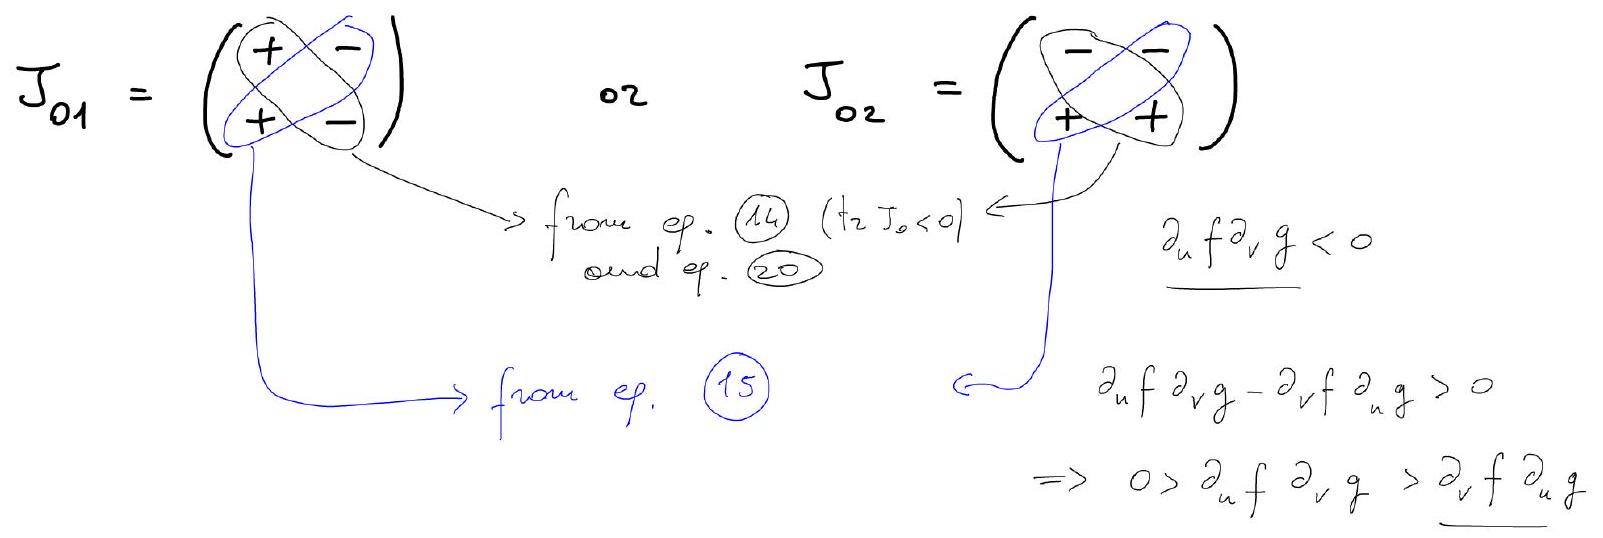
\includegraphics[width=0.5\textwidth]{graphics/2025_10_17_3cf351a4349ae3691080g-11}
    \end{figure}
    on the alternative ones ($v$ activ., $u$ inhib.)
    \begin{DispWithArrows}[displaystyle, format=c]
      J_{03}=-J_{01}=\binom{-+}{-+} \quad J_{04}=-J_{02}=\binom{++}{--}
    \end{DispWithArrows}
    for allowing the emergence of a Turing pattern.
  \item When the linearized equations (see eq. (8)) at
    $\left(u_{0}, v_{0}\right)$ have $J_{0}$ of the form $J_{01}$, we say that
    the system is a pure activator-inhibitor system. From eq. (8) and $J_{01}$
    \begin{figure}[H]
      \centering
      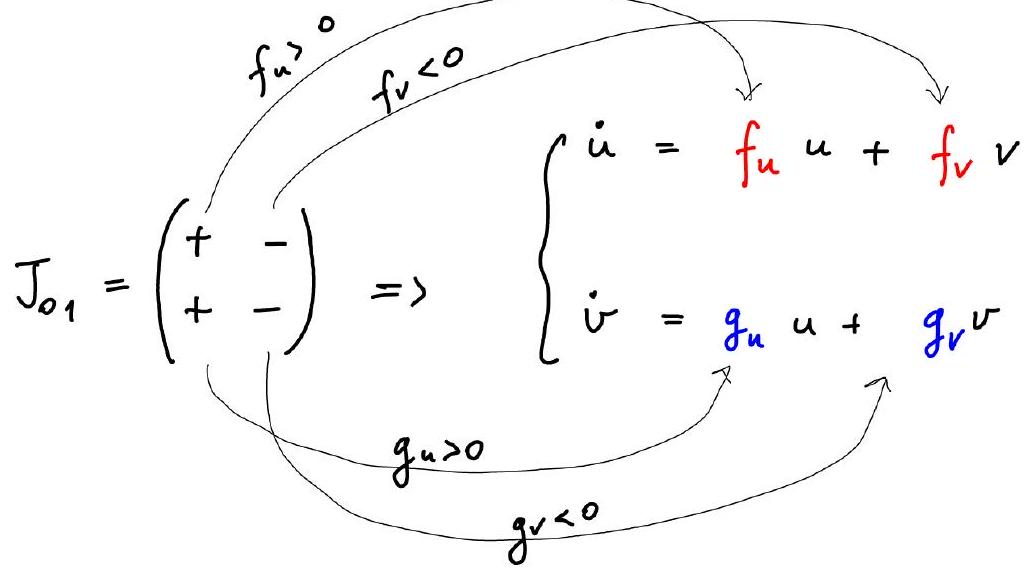
\includegraphics[width=0.5\textwidth]{graphics/2025_10_17_3cf351a4349ae3691080g-12(4)}
    \end{figure}
    \begin{figure}[H]
      \centering
      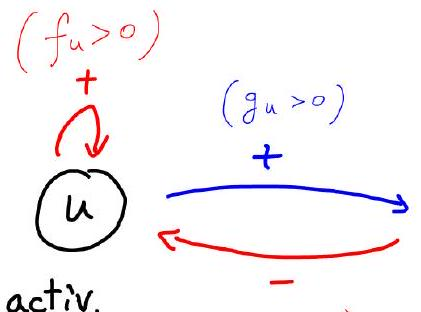
\includegraphics[width=0.5\textwidth]{graphics/2025_10_17_3cf351a4349ae3691080g-12}
    \end{figure}
    (a) At steady state $u$ activates its own production, but $v$ inhibits the
    production of $u$;
    (b) At steady state $u$ also activates the production of $v$, but $v$
    inhibits its own production.

    The equations and diagram show why $u$ is termed ACTIVATOR, while $v$ is
    termed INHIBITOR. Because we also have $D_{2}>D_{1}$ we get short-range
    activation and long-range inhibition.

    In this case $u$ and $v$ grow in phase: (look at the eigenvectors of
    $J_{01}$)
    \begin{figure}[H]
      \centering
      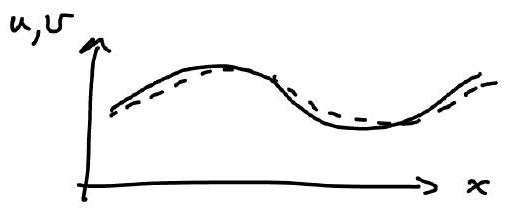
\includegraphics[width=0.5\textwidth]{graphics/2025_10_17_3cf351a4349ae3691080g-12(1)}
    \end{figure}
    In the second case for $J_{02}$:
    \begin{figure}[H]
      \centering
      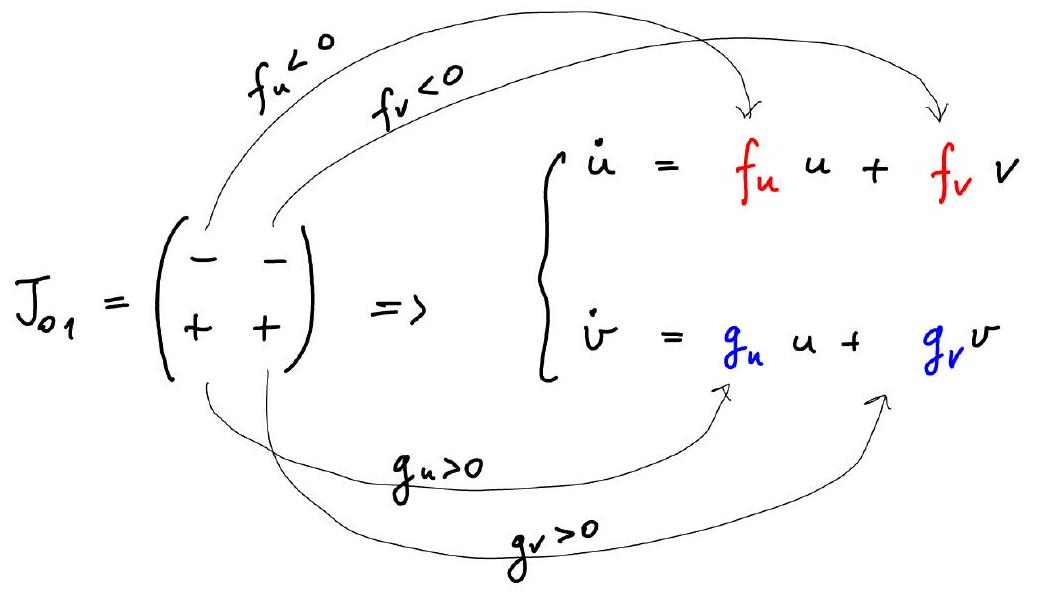
\includegraphics[width=0.5\textwidth]{graphics/2025_10_17_3cf351a4349ae3691080g-12(3)}
    \end{figure}
    \begin{figure}[H]
      \centering
      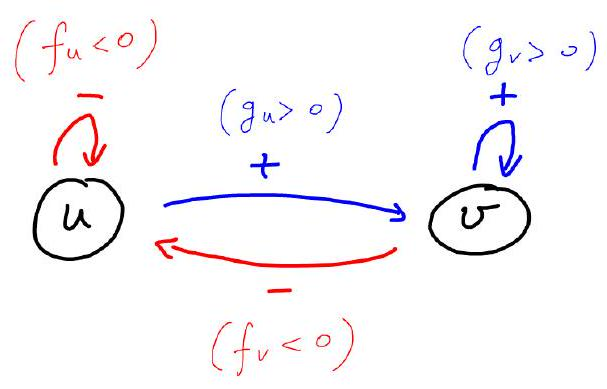
\includegraphics[width=0.5\textwidth]{graphics/2025_10_17_3cf351a4349ae3691080g-12(2)}
    \end{figure}
    (c) At steady state, $u$ inhibits its own production as well as $v$ inhibits
    the production of $u$;
    (d) At steady state, $u$ produces $v$, and $v$ activates itself.

    In this case the system is called cross-activator-inhibitor system and $u$
    and $v$ grow out of phase ($180^{\circ}$)
    \begin{figure}[H]
      \centering
      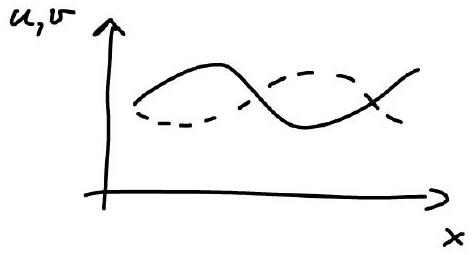
\includegraphics[width=0.5\textwidth]{graphics/2025_10_17_3cf351a4349ae3691080g-13}
    \end{figure}
  \item From eq. (23) it follows that there exists a minimum domain size for
    pattern formation. Indeed, for $L$ sufficiently small, the inequality in
    (23) cannot be satisfied for $n>0$.
  \item As the domain size increases ($L$ becomes larger), the number of viable
    integers also increases and the pattern will become more complicated.
  \item Considerations in (3) and (4) can be extended to higher dimensions,
    where there may occur degeneracy. In $d=2$
    \begin{DispWithArrows}[displaystyle, format=c]
      k^{2}=\left(\frac{n \pi}{L_{x}}\right)^{2}+\left(\frac{m \pi}{L_{y}}\right)^{2} \quad n, m \in \mathbb{N}
    \end{DispWithArrows}
    Because there may exist multiple pairs ($n, m$) which produce the same
    $k^{2}$, in higher dimensions different patterns (say, stripes, checkerboard,
    spots..) may emerge due to different initial conditions, which may combine
    different solutions (on the basis of the non-linear terms).
\end{enumerate}

% Lecture file created by newnote
% Class: Models of Theoretical Physics
% Professor: Azaele Sandro
% Date: 2025-10-17
\lecture{5}{Birth and death Markov processes}{2025-10-17}
\pagelayout{margin}
% --- Start writing here ---

\section{Birth and death Markov processes}
We discuss here a simple class of Markov processes, those that have a set of states that can be labeled with integers. We start from an even simpler discrete Markov process, the birth and death processes which occur in many applications. Then we will deduce results to more general cases.
We start from a situation that is very similar to the random walk. We assume discrete times $t=0, \Delta t, 2 \Delta t, \ldots$ discrete states $x=0, \pm 1, \pm 2 \ldots$ and that jumps are allowed only between nearest neighbors, i.e. from $n$ to $n \pm 1$. For $\Delta t \ll 1$ we call $b_{n} \geqslant 0$ the birth rate, i.e., $b_{n} \Delta t$ is the prob. to jump to $n+1$ at time $t+\Delta t$, given that at time $t$ the state was $n$. (notice that $b_{n}$ does not depend on time, though it could in principle. If it does not, we say that the process is homogeneous). Analogously, $d_{n} \geqslant 0$ is the death rate, i.e. $d_{n} \Delta t$ is the prob. to jump to $n-1$ at time $t+\Delta t$, given that at time $t$ the state was $n$.
We want to calculate the prob. $p(n, t+\Delta t)$ (the propagator).
\begin{figure}[H]
    \centering
    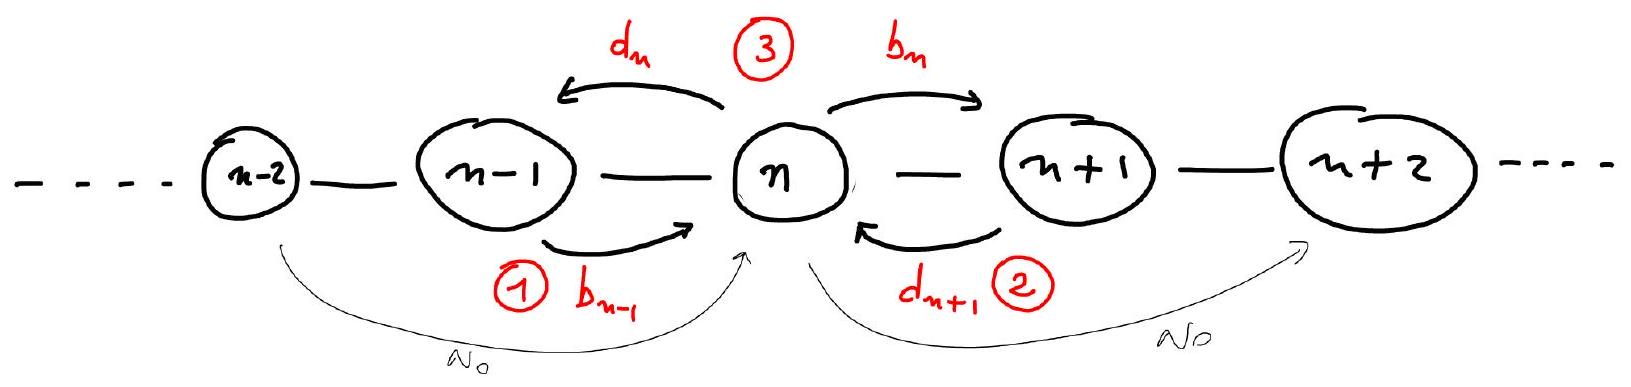
\includegraphics[width=\textwidth]{2025_10_17_3daf2a002a8f5936c90eg-01}
\end{figure}
\begin{DispWithArrows}[displaystyle, format=c]
    p(n, t+\Delta t)=b_{n-1} \Delta t p(n-1, t)+d_{n+1} \Delta t p(n+1, t)+\left[1-\left(b_{n}+d_{n}\right) \Delta t\right] p(n, t)
\end{DispWithArrows}
By Taylor expansions and then taking the limit $\Delta t \rightarrow 0$ we get
\begin{DispWithArrows}[displaystyle, format=c]
    \frac{\partial p_{n}}{\partial t}=b_{n-1} p_{n-1}(t)+d_{n+1} p_{n+1}(t)-\left(b_{n}+d_{n}\right) p_{n}(t)
\end{DispWithArrows}
This is called the master equation of the birth-death process or generation-recombination process.

A few observations:
\begin{enumerate}
    \item The M.E. is a gain-loss equation for the probabilities $p_{n}$;
    \item We have to equip eq. (1) with initial conditions. If We start with $P_{n, n_{0}}\left(t_{0}\right)=\delta_{n, n_{0}}$, then the M.E. is the equation of the propagator of the Markov process, that is
    \begin{DispWithArrows}[displaystyle, format=c]
        P_{n}(t) \equiv P\left(n, t \mid n_{0} t_{0}\right)
    \end{DispWithArrows}
    So one can show (exercise) that $p_{n}(t)$ satisfies the Chapman-Kolmogorov eq. in its differential form. More follows on this.
    \item We can introduce boundary conditions as well. For instance, if $N$ is a reflecting boundary,
    \begin{figure}[H]
        \centering
        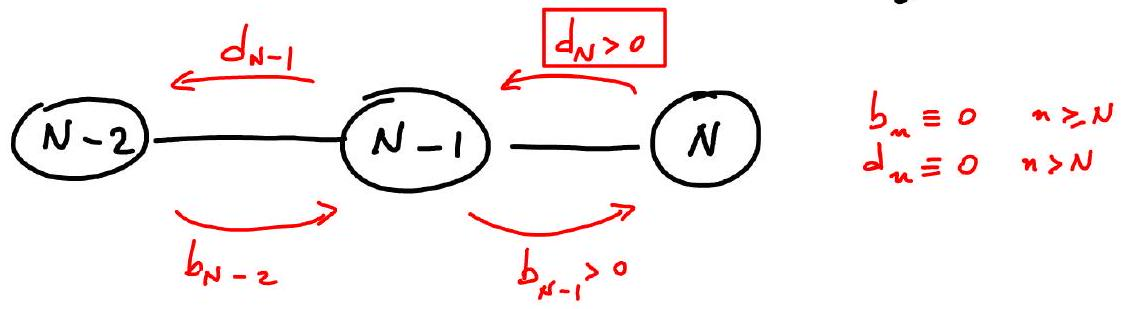
\includegraphics[width=\textwidth]{2025_10_17_3daf2a002a8f5936c90eg-02}
    \end{figure}
    then $b_{n} \equiv 0 \forall n \geqslant N, d_{n} \equiv 0 \forall n>N \quad\left(\right.$ for $n<N, b_{n}$ and $d_{n}$ are $\left.\geqslant 0\right)$ therefore if the state $N$ is reached, it can be left from one side only. $N$ is a reflecting state.

    If $N$ is an absorbing boundary,
    \begin{figure}[H]
        \centering
        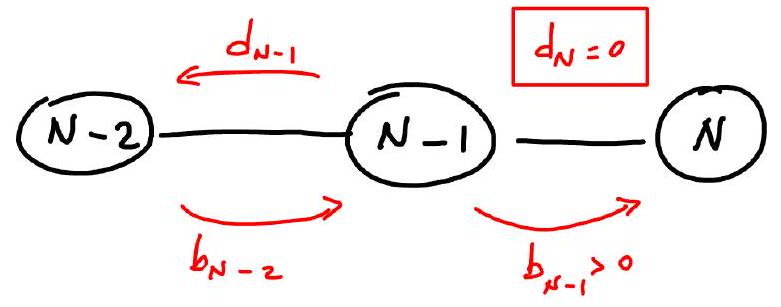
\includegraphics[width=\textwidth]{2025_10_17_3daf2a002a8f5936c90eg-03}
    \end{figure}
    here $d_{N}=0$ which is important, because when the state $N$ is reached, it can no longer be left. We say that $N$ is an absorbing state.
\end{enumerate}

\subsection*{Warning:}
Because of the b.c. We have to be careful with eq. (1) as it holds only when the boundary states are not hit, otherwise it must be changed.
\begin{enumerate}
    \setcounter{enumi}{3}
    \item Notice that eq. (1) is linear and deterministic; indeed we can define a matrix $\mathbb{W}$ whose entries are
    \begin{DispWithArrows}[displaystyle, format=c]
        \mathbb{W}_{m m^{\prime}}=d_{m^{\prime}} \delta_{m, m^{\prime}-1}+b_{m^{\prime}} \delta_{m, m^{\prime}+1}-\left(d_{m}+b_{m}\right) \delta_{m, n^{\prime}}
    \end{DispWithArrows}
    So, if we introduce the vector notation $[\vec{p}(t)]_{n} \equiv p_{n}(t)$ we can write eq. (1) as
    \begin{DispWithArrows}[displaystyle, format=c]
        \left\{\begin{array}{l}\dot{\vec{P}}(t)=\mathbb{W} \vec{P} \\ \vec{P}(0)=\vec{P}_{0}\end{array}\right.
    \end{DispWithArrows}
    and formally the solution reads $\vec{P}(t)=e^{\mathbb{W} t} \vec{P}_{0}$.
    The master equation defined in eq. (4b) holds in general for a continuous time, discrete Markov process as long as $\mathbb{W}$ satisfies the following properties:
    \begin{enumerate}
        \item $W_{n n^{\prime}} \geqslant 0$ for $n \neq n^{\prime}$
        \item $\sum_{m} \mathbb{W}_{m n^{\prime}}=0$ for each $n^{\prime}$ (no abs. bound.)
    \end{enumerate}
\end{enumerate}

\subsection*{The equations for the mean and the variance}
From eq. (1) one can simply derive the eqs. for the time evolution of the mean and the variance. We first multiply eq. (1) by $n$ and sum over $n$: $\langle n\rangle \equiv \sum_{-\infty}^{+\infty} n p_{n}(t)$
\begin{DispWithArrows}[displaystyle, format=c]
    \begin{aligned}
    \frac{d}{d t}\langle n\rangle & =\sum_{-\infty}^{+\infty}\left(n b_{n-1} p_{n-1}-n b_{n} p_{n}+n d_{n+1} p_{n+1}-n d_{n} p_{n}\right) \\
    & =\sum_{n}\left[(n+1) b_{n} p_{n}-n b_{n} p_{n}+(n-1) d_{n} p_{n}-n d_{n} p_{n}\right] \\
    & =\sum_{n}\left(b_{n}-d_{n}\right) p_{n}
    \end{aligned}
\end{DispWithArrows}
\begin{DispWithArrows}[displaystyle, format=c]
    \frac{d}{d t}\langle n\rangle=\left\langle b_{n}\right\rangle-\left\langle d_{n}\right\rangle \quad \begin{array}{ll}
     & \left\langle b_{n}\right\rangle \equiv \sum_{n} b_{n} p_{n} \\
     & \left\langle d_{n}\right\rangle \equiv \sum_{n} d_{n} p_{n}
    \end{array}
\end{DispWithArrows}
with some initial conditions. Notice that this equation has to be equipped with different equations if there is an absorbing or reflecting b.c. Can you find them?

For the evolution of the variance we have to derive an equation for the second moment $\left\langle n^{2}\right\rangle$. We first multiply eq. (1) by $n^{2}$ and then sum over $n$:
\begin{DispWithArrows}[displaystyle, format=c]
    \begin{aligned}
    \frac{d}{d t}\left\langle n^{2}\right\rangle & =\sum_{-\infty}^{+\infty} n^{2}\left(b_{n-1} p_{n-1}+\cdots\right)=\\
    & =\sum_{n}\left((n+1)^{2}-n^{2}\right) b_{n} p_{n}+\sum_{n}\left[(n-1)^{2}-n^{2}\right] d_{n} p_{n} \\
    & =\sum_{n}(2 n+1) b_{n} p_{n}+\sum_{n}(-2 n+1) d_{n} p_{n} \\
    & =2 \sum_{n} n\left(b_{n}-d_{n}\right) p_{n}+\sum_{n}\left(b_{n}+d_{n}\right) p_{n}
    \end{aligned}
\end{DispWithArrows}
Thus
\begin{DispWithArrows}[displaystyle, format=c]
    \frac{d}{d t}\left\langle n^{2}\right\rangle=2\left\langle n\left(b_{n}-d_{n}\right)\right\rangle+\left\langle b_{n}+d_{n}\right\rangle
\end{DispWithArrows}

\subsection*{The equilibrium distribution}
For birth and death process it is possible to calculate the equilibrium distribution of eq. (1) in general. This is not possible for more complicated discrete Markov processes.
We will calculate the distribution for a b/d process defined between 0 (ref. b.c.) and $\infty$.
We can define a stationary flux from $n-1$ to $n$:
\begin{figure}[H]
    \centering
    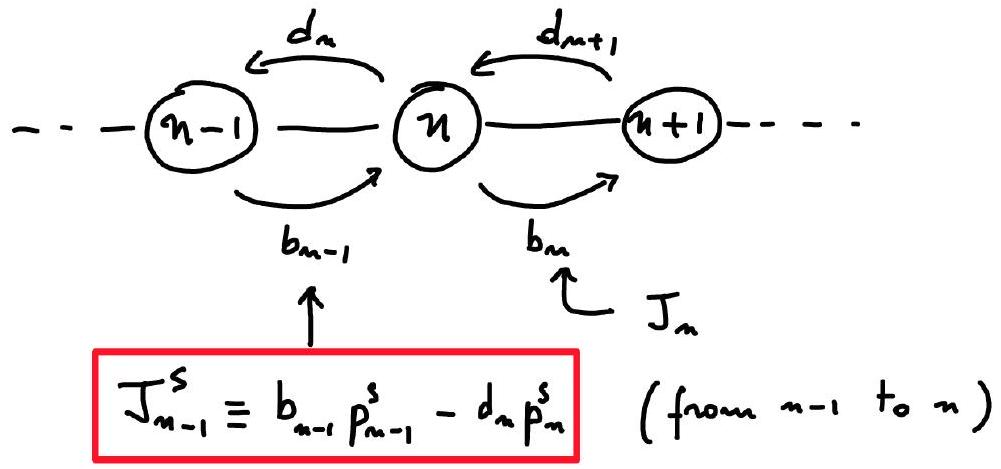
\includegraphics[width=0.5\textwidth]{2025_10_17_3daf2a002a8f5936c90eg-05}
\end{figure}
From eq. (1) we get then
\begin{DispWithArrows}[displaystyle, format=c]
    0=\underbrace{b_{n-1} p_{n-1}^{s}-d_{n} p_{n}^{s}}_{J_{n-1}}+\underbrace{d_{n+1} p_{n+1}^{s}-b_{n} p_{n}^{s}}_{-J_{n}}
\end{DispWithArrows}
hence $J_{n}=J_{n-1}=\ldots=J_{0} = b_{-1} p_{-1}^{s}-d_{0} p_{0}^{s}=0$ (ref. b.c. at $n=0$)
then
\begin{DispWithArrows}
    \begin{gathered}
    J_{n}=b_{n-1} p_{n-1}^{s}-d_{n} p_{n}^{s}=0 \Rightarrow b_{n-1} p_{n-1}^{s}=d_{n} p_{n}^{s} \quad \text{DETAILED BALANCE} \\
    p_{n}^{s}=\frac{b_{n-1}}{d_{n}} p_{n-1}^{s}=\frac{b_{n-1}}{d_{n}} \frac{b_{n-2}}{d_{n-1}} p_{n-2}^{s}=\ldots
    \end{gathered}
\end{DispWithArrows}
\begin{DispWithArrows}[displaystyle, format=c]
    p_{n}^{s}=\prod_{i=1}^{n} \frac{b_{i-1}}{d_{i}} p_{0}^{s} \quad \text { for } n=1,2, \ldots
\end{DispWithArrows}
because of normalization, $\left(p_{0}^{s}\right)^{-1}=1+\sum_{n=1}^{\infty} \prod_{i=1}^{n} \frac{b_{i-1}}{d_{i}}$; $p_{n}^{s}$ exists if $p_{0}^{s}<\infty$. The same approach can be used for a finite number of states $n=1, \ldots, N$.

\subsection*{Simple yet important birth and death processes}
\subsubsection*{Poisson process}
This process is defined by the rates $b_{n}=\lambda, d_{n}=0$, where $n=0,1, \ldots$ So the M.E. is
\begin{DispWithArrows}[displaystyle, format=c]
    \left\{\begin{array}{l}\dot{p}_{n}=\lambda\left(p_{n-1}-p_{n}\right) \\ p_{n}(0)=\delta_{n, 0}\end{array}\right.
\end{DispWithArrows}
Ex: show that the mean satisfies the eq. $\frac{d}{d t}\langle n\rangle=\lambda$ and so $\langle n(t)\rangle=n_{0}+\lambda t$ if $p_{n}(0)=\delta_{n, n_{0}}$.

We solve eq. (8) with the method of the generating function:
\begin{DispWithArrows}[displaystyle, format=c]
    g(z, t) \equiv \sum_{n=0}^{\infty} z^{n} p_{n}(t)
\end{DispWithArrows}
So from eq. (8) we get an eq. for $g$:
\begin{DispWithArrows}[displaystyle, format=c]
    \left\{\begin{array}{l}\frac{\partial}{\partial t} g(z, t)=\lambda(z-1) g(z, t) \quad\left(g(1, t)=\sum_{n} p_{n}(t)=1\right) \\ g(z, 0)=\sum_{n} z^{n} \delta_{n, 0}=1\end{array}\right.
\end{DispWithArrows}
The solution of (9) is then
\begin{DispWithArrows}[displaystyle, format=c]
    g(z, t)=e^{\lambda(z-1) t}=e^{-\lambda t} \sum_{n=0}^{\infty} \frac{(\lambda t)^{n}}{n!} z^{n}
\end{DispWithArrows}
hence
\begin{DispWithArrows}[displaystyle, format=c]
    p_{n}(t)=e^{-\lambda t} \frac{(\lambda t)^{n}}{n!}
\end{DispWithArrows}
Show that $\operatorname{var}(n(t))=\lambda t$.

\subsubsection*{Radioactive decay}
Initially the system consists of $N_{0}$ radioactive particles which decay at rate $\gamma$. Therefore, if at time $t$ there are $n$ surviving particles, then in the following $\Delta t$ time the probability of one decay is $\gamma n \Delta t$ and more than one decay is $o(\Delta t)$. Thus $d_{n}=\gamma n$ and $b_{n}=0$ and the M.E. is
\begin{DispWithArrows}[displaystyle, format=c]
    \left\{\begin{array}{l}\dot{p}_{n}=\gamma(n+1) p_{n+1}(t)-\gamma n p_{n}(t) \quad n=0,1 \ldots N_{0}-1 \quad \text{a.b.c. at } n=0 . \\ \dot{p}_{N_{0}}=-\gamma N_{0} p_{N_{0}}(t) \\ p_{n}(0)=\delta_{n, N_{0}}\end{array}\right.
\end{DispWithArrows}
Ex: show that $\frac{d}{d t}\langle n\rangle=-\gamma\langle n\rangle$, so $\langle n(t)\rangle=N_{0} e^{-\gamma t}$.
With the generating function $g(z, t)=\sum_{n=0}^{N_{0}} z^{n} p_{n}(t)$ we get
\begin{DispWithArrows}[displaystyle, format=c]
    \frac{\partial g(z, t)}{\partial t}=\gamma(1-z) \frac{\partial}{\partial z} g(z, t) \quad \begin{aligned} & g(1, t)=1 \\ & g(z, 0)=z^{N_{0}} \end{aligned}
\end{DispWithArrows}
Notice that $h(z, t)=\varepsilon(t)(1-z)+1$ leads to $\dot{\varepsilon}=-\gamma \varepsilon$, namely $\varepsilon(t)=\varepsilon_{0} e^{-\gamma t}$, so $h(1, t)=1$, but $h(z, 0)=\varepsilon_{0}(1-z)+1 \neq z^{N_{0}}$. However, take $g$ as a function of $h$, i.e. $g(z, t)=f(h(z, t))$, we get from (11)
\begin{DispWithArrows}[displaystyle, format=c]
    \frac{\partial g}{\partial t}=\frac{d f}{d h} \frac{\partial h}{\partial t} \quad , \quad \frac{\partial g}{\partial z}=\frac{d f}{d h} \frac{\partial h}{\partial z}
\end{DispWithArrows}
and $\frac{d f}{d h}$ simplifies, because it occurs on both sides of eq. (11). We can then use $f$ to satisfy the i.c.: $f(a)=a^{N_{0}}$ does the job. We take $g=\left(\varepsilon_{0} e^{-\gamma t}(1-z)+1\right)^{N_{0}}$ where $\varepsilon_{0}=-1$. Eventually, the sol, is
\begin{DispWithArrows}[displaystyle, format=c]
    g(z, t)=\left(e^{-\gamma t}(z-1)+1\right)^{N_{0}}
\end{DispWithArrows}
We have now to invert this relation to get $p_{n}(t)$
\begin{DispWithArrows}[displaystyle, format=c]
    g(z, t)=\left(e^{-\gamma t} z+\left(1-e^{-\gamma t}\right)\right)^{N_{0}}=\sum_{n=0}^{N_{0}}\binom{N_{0}}{n}\left(1-e^{-\gamma t}\right)^{N_{0}-n} e^{-n \gamma t} z^{n}
\end{DispWithArrows}
which gives
\begin{DispWithArrows}[displaystyle, format=c]
    p_{n}(t)=\binom{N_{0}}{n} e^{-n \gamma t}\left(1-e^{-\gamma t}\right)^{N_{0}-n}
\end{DispWithArrows}
We can interpret this eq. in this way: $e^{-n \gamma t}$ is the prob. that $n$ particles have survived (i.e., not decayed yet) by time $t,\left(1-e^{-\gamma t}\right)^{N_{0}-n}$ is the prob. that $N_{0}-n$ particles have decayed by time $t$. We also need the factor $\binom{N_{0}}{n}$ because the specific identity of the particles is not important, then there are $\binom{N_{0}}{n}$ ways to select $n$ surviving particles out of $N_{0}$.

\subsubsection*{Furry process}
A cosmic electron enters an absorbing material (like lead...) and branches into multiple particles (an electron may emit a photon which may then produce an $e^{+}-e^{-}$ pair). So a cascade of secondary particles is produced which generates a shower of final particles. This process can be described by a birth and death process where $b_{n}=\gamma n$ and $d_{n}=0, n=1,2, \ldots$
The M.E. is then
\begin{DispWithArrows}[displaystyle, format=c]
    \left\{\begin{array}{l}\dot{p}_{n}=\gamma(n-1) p_{n-1}-\gamma n p_{n} \\ p_{n}(0)=\delta_{n, 1}\end{array}\right.
\end{DispWithArrows}
Show as before that
\begin{DispWithArrows}[displaystyle, format=c]
    \begin{aligned}
    & \langle n(t)\rangle=e^{\gamma t} \\
    & \operatorname{Var}(n(t))=e^{\gamma t}\left(e^{\gamma t}-1\right)
    \end{aligned}
\end{DispWithArrows}
Finally:
\begin{DispWithArrows}[displaystyle, format=c]
    p_{n}(t)=e^{-\gamma t}\left(1-e^{-\gamma t}\right)^{n-1}
\end{DispWithArrows}
try to interpret the result.

\subsubsection*{The contact process}
Let us assume that a population of $N$ individuals can be divided into two categories according to whether they are infected or not (but are susceptible any way). If an indiv. has not yet caught the infection, may catch it from any of of the $n$ infected ones (uniformly at random).
We can write down the transition rate from $n$ to $n+1$ infected individuals; if the number of infected ind. increases by one, then one healthy ind. must get in contact with an infected one:
\begin{enumerate}
    \item first, we have to pick one healthy indiv.
    \begin{DispWithArrows}
        b_{n}=\tilde{\beta} \frac{N-n}{N} \frac{n}{N-1}=\frac{\beta}{N} n(N-n)
    \end{DispWithArrows}
    \item second, the healthy ind. have to encounter an infected one.
\end{enumerate}
We then assume that an infected individual recovers at rate $\gamma$. then the transition rate from state $n$ to $n-1$ is $d_{n}=\gamma n$. Notice that $b_{0}=0=d_{0}$ ($n=0$ is an absorbing state) and $b_{N}=0, d_{N} \neq 0$ ($n=N$ is a reflecting state) and we have to set $d_{N+1}=0$.
Notice that the rates $b_{n}$ and $d_{n}$ can be written as a function of $x=\frac{n}{N}: b_{x}=N \beta x(1-x), d_{x}=N \gamma x$.
As $N$ becomes large, the variations in $n$ become small and so one hopes to describe $x$ as a continuous variable. Making this limit rigorous is tricky (Kurtz's theorem), but one can anyway guess the limiting equation. the important assumption is the existence of a typical scale of the system (in this case $N$) and that the parameters (here $\beta$ and $\gamma$) scale appropriately with $N$.

The master equation has a form
\begin{DispWithArrows}[displaystyle, format=c]
    \dot{q}_{n}(t)=b_{\frac{n-1}{N}} q_{n-1}+d_{\frac{n+1}{N}} q_{n+1}-\left(b_{\frac{n}{N}}+d_{\frac{n}{N}}\right) q_{n}
\end{DispWithArrows}
In the continuous limit $q_{n}(t)$ becomes a PDF of $x$, so we write
\begin{DispWithArrows}[displaystyle, format=c]
    q_{n}(t)=\frac{1}{N} p(x, t) \quad \text { for large } N
\end{DispWithArrows}
So eq. (15) becomes
\begin{DispWithArrows}[displaystyle, format=c]
    \dot{p}(x, t)=b_{x-\frac{1}{N}} p\left(x-\frac{1}{N}, t\right)+d_{x+\frac{1}{N}} p\left(x+\frac{1}{N}, t\right)-\left(b_{x}+d_{x}\right) p(x, t)
\end{DispWithArrows}
As $\frac{1}{N}$ is small, we can Taylor expand eq. (16):
\begin{DispWithArrows}[displaystyle, format=c]
    \begin{aligned}
    & b_{x-\frac{1}{N}} p\left(x-\frac{1}{N}\right)-b_{x} p(x)=-\frac{1}{N} \frac{d}{d x}\left(b_{x} p_{x}\right)+\frac{1}{2} \frac{1}{N^{2}} \frac{d^{2}}{d x^{2}}\left(b_{x} p_{x}\right)+\text { h.o.t. } \\
    & d_{x+\frac{1}{N}} p\left(x+\frac{1}{N}\right)-d_{x} p(x)=\frac{1}{N} \frac{d}{d x}\left(d_{x} p_{x}\right)+\frac{1}{2} \frac{1}{N^{2}} \frac{d^{2}}{d x^{2}}\left(d_{x} p_{x}\right)+\text { h.o.t. }
    \end{aligned}
\end{DispWithArrows}
Therefore
\begin{DispWithArrows}[displaystyle, format=c]
    \dot{p}(x, t)=-\frac{1}{N} \frac{\partial}{\partial x}\left[\left(b_{x}-d_{x}\right) p_{x}\right]+\frac{1}{2 N^{2}} \frac{\partial^{2}}{\partial x^{2}}\left[\left(b_{x}+d_{x}\right) p_{x}\right]+\text { h.o.t. }
\end{DispWithArrows}
as $b_{x}=N \beta x(1-x)$ and $d_{x}=N \gamma x$ we get the F.P. equation
\begin{DispWithArrows}[displaystyle, format=c]
    \dot{p}(x, t)=-\frac{\partial}{\partial x}[(\beta x(1-x)-\gamma x) p]+\frac{1}{2 N} \frac{\partial^{2}}{\partial x^{2}}[(\beta x(1-x)+\gamma x) p]
\end{DispWithArrows}
which corresponds to an Itô SDE: ($0<x<1$)
\begin{DispWithArrows}[displaystyle, format=c]
    d x=(\beta x(1-x)-\gamma x) d t+\sqrt{\frac{\beta x(1-x)+\gamma x}{N}} d B(t)
\end{DispWithArrows}
Fluctuations are of order $N^{-1 / 2}$.

In general, although the equation and its derivation are not rigorous, a birth and death process may be well approximated by the F.P. equation
\begin{DispWithArrows}[displaystyle, format=c]
    \dot{p}(x, t)=-\frac{\partial}{\partial x}\left[\left(b_{x}-d_{x}\right) p_{x}\right]+\frac{1}{2} \frac{\partial^{2}}{\partial x^{2}}\left[\left(b_{x}+d_{x}\right) p_{x}\right]
\end{DispWithArrows}
at least in some region of the parameter space. It is anyway expected that eq. (19) is very inaccurate close to (possible) boundaries or when $N$ (or other typical param.) is small. This approx is called Kramers-Moyal expansion and has several generalizations. Other more rigorous approximations exist (like the van Kampen approximation (see p. 244, van Kampen) or the WKB expansion... which are more accurate but more difficult as well.

Back to the contact process.
The mean of the infected individuals, $\rho(t) \equiv \mathbb{E}(x(t))$, satisfies (see eq. (18b))
\begin{DispWithArrows}[displaystyle, format=c]
    \dot{\rho}=(\beta-\gamma) \rho-\beta \mathbb{E}\left(x(t)^{2}\right)
\end{DispWithArrows}
This equation is not closed and cannot be solved, unless we know the behavior of $\mathbb{E}\left(x^{2}\right)$. The mean depends on the fluctuations. However, the eq. for $\mathbb{E}\left(x^{2}\right)$ depends on $\mathbb{E}\left(x^{3}\right)$, so we obtain an infinite chain of equations which cannot be solved unless we solve the full F.P. equation.
One way to obtain some information is to resort to the moment closure: if fluctuations are small, then
\begin{DispWithArrows}
    \mathbb{E}\left(x^{2}(t)\right) \simeq \mathbb{E}(x(t))^{2}=\rho(t)^{2}
\end{DispWithArrows}
Under this approximation
\begin{DispWithArrows}[displaystyle, format=c]
    \dot{\rho}=(\beta-\gamma) \rho-\beta \rho^{2}
\end{DispWithArrows}
which is a logistic equation that can be solved as we have seen at the beginning of the course.
There are two steady states ($\dot{\rho}=0$): $\rho^{*}=0$ and $\bar{\rho}=\frac{\beta-\gamma}{\beta}$. What is their meaning?
Let's look at their stability:
\begin{DispWithArrows}[displaystyle, format=c]
    \frac{d \dot{\rho}}{d \rho}=\beta-\gamma-\left.2 \beta \rho\right|_{\rho=\rho^{s t}}=\left\{\begin{array}{cc}
    \beta-\gamma & \rho=\rho^{*}=0 \\ \gamma-\beta & \rho=\bar{\rho}=\frac{\beta-\gamma}{\beta}\end{array}\right.
\end{DispWithArrows}
\begin{itemize}
    \item Therefore $\rho=0$ is stable as $\beta<\gamma$ (and $\bar{\rho}$ is unstable)
    \begin{figure}[H]
        \centering
        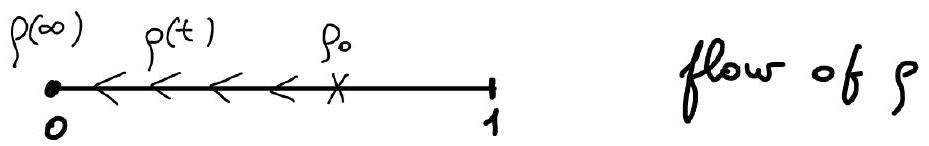
\includegraphics[width=0.5\textwidth]{2025_10_17_3daf2a002a8f5936c90eg-12}
    \end{figure}
    after some time, the eq. is well approximated by
    \begin{DispWithArrows}[displaystyle, format=c]
        \dot{\rho}=(\beta-\gamma) \rho \quad \rightarrow \rho(t)=\tilde{\rho} e^{-|\beta-\gamma| t} \rho \rightarrow_{t}
    \end{DispWithArrows}
    \item Viceversa, $\bar{\rho}=\frac{\beta-\gamma}{\beta}(>0)$ is stable as $\beta>\gamma$ (and $\rho=0$ is unstable)
    \begin{figure}[H]
        \centering
        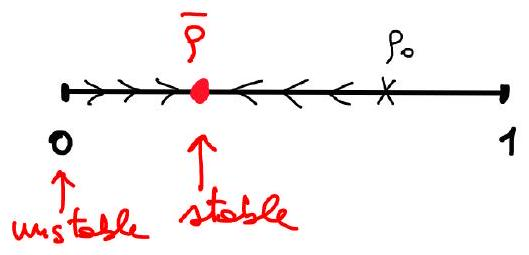
\includegraphics[width=0.5\textwidth]{2025_10_17_3daf2a002a8f5936c90eg-12(1)}
    \end{figure}
    after some time, the eq. is well approximated by $\rho(t)=\bar{\rho}+y(t)$ ($y \ll \bar{\rho}$)
    \begin{DispWithArrows}[displaystyle, format=c]
        \dot{\rho}=-(\beta-\gamma)(\bar{\rho}-\rho) \quad \rightarrow \quad \rho(t)=\bar{\rho}+\tilde{\rho} e^{-|\beta-\gamma| t}
    \end{DispWithArrows}
\end{itemize}
\begin{figure}[H]
    \centering
    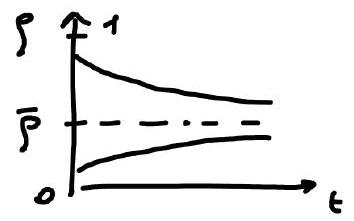
\includegraphics[width=0.5\textwidth]{2025_10_17_3daf2a002a8f5936c90eg-12(2)}
\end{figure}
So the characteristic time scale is $|\beta-\gamma|^{-1}$ in both cases.
Of course this is summarized by the full solution:
\begin{DispWithArrows}[displaystyle, format=c]
    \rho(t)=\frac{\bar{\rho}}{1+\left(\frac{\bar{\rho}}{\rho_{0}}-1\right) e^{(\gamma-\beta) t}}=\frac{(\beta-\gamma) \rho_{0}}{\beta \rho_{0}+\left(\beta-\gamma-\beta \rho_{0}\right) e^{(\gamma-\beta) t}}
\end{DispWithArrows}
where $\rho_{0}$ is the initial condition for the density ($0<\rho_{0}<1$) of infected individuals.
The phase diagram of this process reads:
\begin{figure}[H]
    \centering
    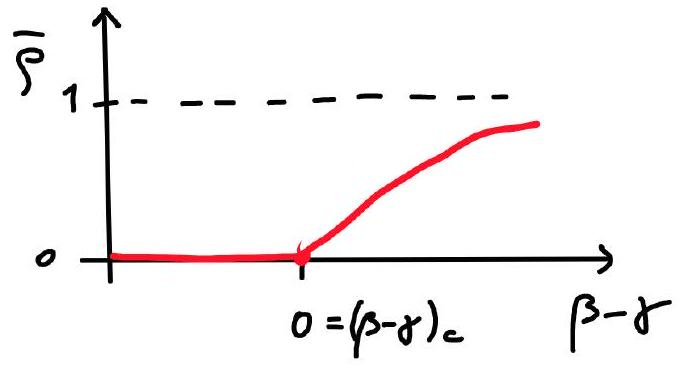
\includegraphics[width=0.5\textwidth]{2025_10_17_3daf2a002a8f5936c90eg-13}
\end{figure}
\begin{DispWithArrows}[displaystyle, format=c]
    \begin{gathered}
    \bar{\rho} \sim(\beta-\gamma)^{1} \\
    \beta>\gamma
    \end{gathered}
\end{DispWithArrows}
At the critical point $\beta=\gamma$:
\begin{DispWithArrows}[displaystyle, format=c]
    \dot{\rho}=-\beta \rho^{2} \quad \rightarrow \quad \rho(t)=\frac{\rho_{0}}{1+\beta t} \sim \frac{1}{t} \quad t \gg \beta^{-1}
\end{DispWithArrows}
the decay is no longer exponential but power law: critical slowing down.

Exercise: the discrete random walk in continuous time is governed by the master equation (symmetric R.W.)
\begin{DispWithArrows}[displaystyle, format=c]
    \dot{p}_{n}=p_{n+1}+p_{n-1}-2 p_{n} \quad p_{n}(0)=\delta_{n, 0}
\end{DispWithArrows}
Show that the generating function $F(z, t)=\sum_{-\infty}^{+\infty} z^{n} p_{n}(t)$ satisfies
\begin{DispWithArrows}[displaystyle, format=c]
    \dot{F}=\left(z+\frac{1}{z}-2\right) F
\end{DispWithArrows}
so the solution is $F(z, t)=\exp \left[t\left(z+z^{-1}-2\right)\right]$. From this find
\begin{DispWithArrows}[displaystyle, format=c]
    p_{n}(t)=e^{-t} \sum_{\substack{l \geqslant 0 \\ l+m \geqslant 0}} \frac{t^{2 l+m}}{(l+m)!l!}
\end{DispWithArrows}
Find the K.M. expansion of the M.E. and find its solution.

\subsection*{A simple chemical reaction}
Consider the reaction
\begin{DispWithArrows}[displaystyle, format=c]
    X \underset{k_{2}}{\stackrel{k_{1}}{\rightleftarrows}} A
\end{DispWithArrows}
where the product $A$ is not affected by $x$ and it does not decrease its quantity even though it produces particles at rate $k_{2}$. We are interested into the stochastic evolution of $X$: the r.v. $n$. From a simple application of the mass action law we get the evolution of the deterministic value $\rho(t)=\mathbb{E}(n(t))$:
\begin{DispWithArrows}[displaystyle, format=c]
    \dot{\rho}=-k_{1} \rho+k_{2} a
\end{DispWithArrows}
where $a$ is a constant.

We want now to get information about the fluctuations: If at time $t$ there are $n$ particles of type $x$, then the prob. that at time $t+\Delta t$ there is one more is given by $k_{2} a \Delta t$, and one less is $k_{1} n \Delta t$. So we get a birth and death process with rates
\begin{DispWithArrows}[displaystyle, format=c]
    \begin{aligned}
    & b_{n}=k_{2} a \equiv b \quad(\text { a constant }) \\
    & d_{n}=k_{1} n
    \end{aligned}
\end{DispWithArrows}
where $n=0,1, \ldots$
It is not difficult to find that the equilibrium distribution of $n$ (from eq. (7))
\begin{DispWithArrows}[displaystyle, format=c]
    p_{n}^{s t}=\frac{\lambda^{n}}{n!} e^{-\lambda} \quad \lambda=\frac{k_{2}a}{k_{1}}
\end{DispWithArrows}
what is the difference between this solution and eq. (10)?
The average is also (from eq. (5))
\begin{DispWithArrows}[displaystyle, format=c]
    \frac{d}{d t}\langle n\rangle=b-k_{1}\langle n\rangle
\end{DispWithArrows}
which is like eq. 23.
Ex: find the M.E. for the chemical reaction $A+x \xrightarrow{k_{1}} 2 x, x \stackrel{k_{2}}{\stackrel{k_{3}}{\rightleftarrows}} B$. and compare the results with those from the law of mass action.

\subsection*{Exact simulation of a birth and death process: the Gillespie's algorithm}
The M.E. in eq. (1) governs a b/d process whose trajectories can be generated exactly (up to machine numerical errors). The M.E. includes all the info we need as it defines the process itself. We know that it is a Markov process therefore the information that we possess at time $t$ is enough to define what happens in the future.
We need two pieces of info to generate a path:
\begin{enumerate}
    \item What is the time of the next event (either birth or death)?
    \item What is the nature of the event, given that it occurs? namely, what is the probability that it is a birth/death?
\end{enumerate}
If we can answer these two questions then we know when and how the path changes.
Let's define $q_{0}(\tau \mid n)$ as the probability that no events will occur within the interval $[0, \tau)$, given that the system was in the state $n$ at time $t=0$ (as the process is homogeneous, $t=0$ is not a restrictive assumption).
Notice that if $T$ is the (random) time when the next event (birth or death) will occur, then $q_{0}(\tau \mid n)=P(T>\tau \mid n)$.
We build up an equation for $q_{0}(\tau \mid n)$ by using the Markov assumption and that the process is a b/d process:
The prob. that there are no events in the interval $[0, \tau+\Delta \tau)$ is given by the prob. that no events occur within $[0, \tau)$ and neither occur in $[\tau, \tau+\Delta \tau)$:
\begin{DispWithArrows}[displaystyle, format=c]
    q_{0}(\tau+\Delta \tau \mid n)=q_{0}(\tau \mid n)\left(1-b_{n} \Delta \tau-d_{n} \Delta \tau\right)
\end{DispWithArrows}
Therefore as $\Delta \tau \rightarrow 0$
\begin{DispWithArrows}
    \left\{\begin{aligned}
    \frac{d q_{0}(\tau \mid n)}{d \tau} & =-\left(b_{n}+d_{n}\right) q_{0}(\tau \mid n) \\
    q_{0}(0 \mid n) & =1
    \end{aligned}\right.
\end{DispWithArrows}
hence
\begin{DispWithArrows}[displaystyle, format=c]
    q_{0}(\tau \mid n)=e^{-\left(b_{n}+d_{n}\right) \tau}
\end{DispWithArrows}
Now we can calculate $q_{+}(\tau \mid n) \Delta \tau$, namely, the probability that a birth occurs between $\tau$ and $\tau+\Delta \tau$ if the system was in state $n$. This is simply
\begin{DispWithArrows}[displaystyle, format=c]
    q_{+}(\tau \mid n) \Delta \tau=e^{-\left(b_{n}+d_{n}\right) \tau} b_{n} \Delta \tau
\end{DispWithArrows}
prob. of no events up to time $\tau$ prob. of 1 birth event between $\tau$ and $\tau+\Delta \tau$

Therefore the PDF is
\begin{DispWithArrows}[displaystyle, format=c]
    q_{+}(\tau \mid n)=b_{n} e^{-\left(b_{n}+d_{n}\right) \tau}
\end{DispWithArrows}
and for a death event
\begin{DispWithArrows}[displaystyle, format=c]
    q_{-}(\tau \mid n)=d_{n} e^{-\left(b_{n}+d_{n}\right) \tau}
\end{DispWithArrows}
and the PDF of any event (either birth or death) is therefore
\begin{DispWithArrows}[displaystyle, format=c]
    q_{1}(\tau \mid n)=\left(b_{n}+d_{n}\right) e^{-\left(b_{n}+d_{n}\right) \tau}
\end{DispWithArrows}
This means that the PDF of an event is exponentially distributed with mean time $\langle\tau(n)\rangle=\left(b_{n}+d_{n}\right)^{-1}$ (show this). Of course, we assume that the state $n$ is not absorbing, i.e. $b_{n}+d_{n}>0$.

Now $q_{+}(\tau \mid n) \Delta \tau=\left(\begin{array}{c} \text{prob. of a birth event,} \\ \text{given that an event occurs} \\ \text{between } \tau \text{ and } \tau+\Delta \tau\end{array}\right)\binom{\text { prob. that an event occurs }}{\text { between } \tau \text{ and } \tau+\Delta \tau}$
From eqs. (27) we get
\begin{DispWithArrows}[displaystyle, format=c]
    q_{+}(\tau \mid n) \Delta \tau=\frac{b_{n}}{b_{n}+d_{n}}\left(b_{n}+d_{n}\right) e^{-\left(b_{n}+d_{n}\right) \tau} \Delta \tau
\end{DispWithArrows}
prob. of a birth event, given that an event occurs between $\tau$ and $\tau+\Delta \tau$ when the state is $n$
prob. that an event occurs (birth or death) between $\tau$ and $\tau+\Delta \tau$ when the state is $n$

Eq. (30) suggests an algorithm for simulating a path from the master equation (1):

\subsection*{Gillespie's algorithm}
(1) Initialize the system at time $t=0$, starting at state $n_{0}$:
(2) If $b_{n}+d_{n}>0$, generate the time $\tau$ when the next event will occur. So you have to draw a random number from the exponential distribution (29), or equivalently (show this)
\begin{DispWithArrows}[displaystyle, format=c]
    \tau=\frac{1}{b_{n}+d_{n}} \ln \left(\frac{1}{r}\right)
\end{DispWithArrows}
Where $r$ is a random number uniformly distributed in $(0,1)$. Update the time
\begin{DispWithArrows}[displaystyle, format=c]
    t_{\text {new }}=t_{\text {old }}+\tau
\end{DispWithArrows}
$t_{\text {old }}$ is the time when the state was $n$;

If $b_{n}+d_{n}=0$, stop the program as $t_{\text {old }}$ is the extinction time and $n$ is an absorbing state.
(3) Compute whether the next event will be a birth or a death.

As before, let $n$ be the state at time $t_{\text {old }}$. If $b_{n}+d_{n}>0$, generate a random number $u$ uniformly distributed in $(0,1)$.
\begin{itemize}
    \item According to eq. (30), if $u<\frac{b_{n}}{b_{n}+d_{n}}$, then the next event will be a birth. Update the state $n_{\text {new }}=n+1$
    \item Otherwise, the next event will be a death so the update is $n_{\text {new }}=n-1$.
    Of course, if $b_{n}+d_{n}=0$ there cannot be any further update and $n$ is the final absorbing state.
\end{itemize}
(4) Repeat the steps (2) and (3) as needed.

\subsection*{More general discrete Markov processes}
It is not difficult to generalize the considerations that we used for the birth and death processes to continuous time Markov processes where multiple jumps are allowed. Calculation are more difficult but the conceptual framework is similar. The M.E. can be deduced from the Chapman-Kolmogorov equation, but it can also be guessed as we did. Take $n \in E \subseteq \mathbb{Z}$.
Let $T\left(n^{\prime} \mid n\right) \Delta t$ be the probability to jump to state $n^{\prime}(\neq n)$ at time $t+\Delta t$, given that the system was in state $n$ at time $t$.
So $T\left(n^{\prime} \mid n\right) \geqslant 0$ is the corresponding jumping rate. $T$ could depend on time $t$, but we consider the simpler case in which it does not. We can visualize this as follows
\begin{figure}[H]
    \centering
    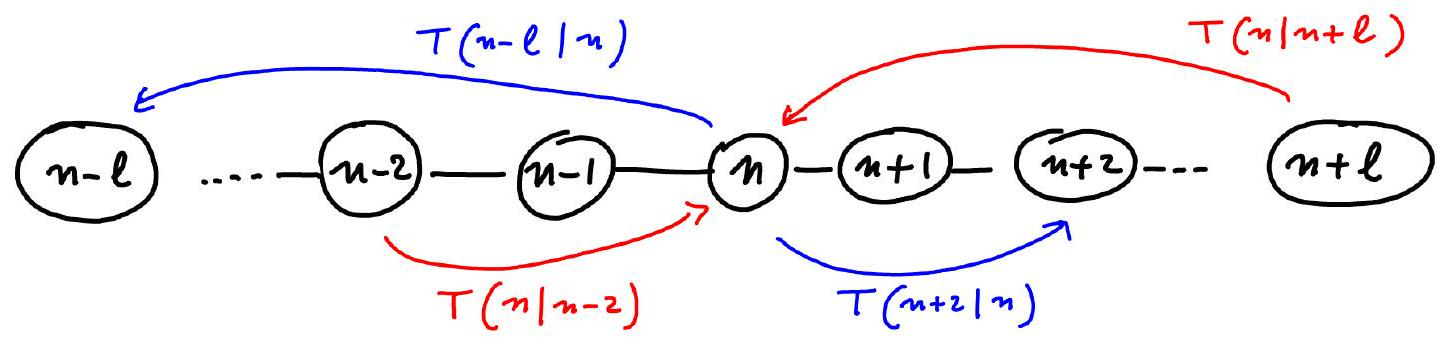
\includegraphics[width=0.5\textwidth]{2025_10_17_3daf2a002a8f5936c90eg-19}
\end{figure}
The M.E. for the propagator $p\left(n, t \mid n_{0}, t_{0}\right)$ is then
\begin{DispWithArrows}[displaystyle, format=c]
    P(n, t+\Delta t)=\underbrace{\sum_{m \neq n} T(n \mid m) \Delta t}_{\substack{\text { probability to } \\ \text { jump from any state } m \neq n \\ \text{ into the state } n}} P(m, t)+\underbrace{\left(1-\sum_{m \neq n} T(m \mid n) \Delta t\right)}_{\substack{\text{probability to} \\ \text{remain in the state } n}} P(n, t)
\end{DispWithArrows}
Therefore as $\Delta t \rightarrow 0$ the Master Equation becomes
\begin{DispWithArrows}[displaystyle, format=c]
    \frac{\partial}{\partial t} p(n, t)=\sum_{m}[T(n \mid m) p(m, t)-T(m \mid n) p(n, t)]
\end{DispWithArrows}
notice that we have included the state $n$ in the sum (why?).

As usual eq. (31) must be equipped with initial conditions $P\left(n, t_{0} \mid n_{0}, t_{0}\right)=\delta_{n, n_{0}}$ and, possibly, some boundary conditions.

Exercise: - Show that $\sum_{n} p(n, t)=1$.
\begin{itemize}
    \item Define the $l$-th jump moment as
    \begin{DispWithArrows}[displaystyle, format=c]
        \mu_{l}(n)=\sum_{m}(m-n)^{l} T(m \mid n) \quad l \geqslant 0
    \end{DispWithArrows}
    Show then that
    \begin{DispWithArrows}[displaystyle, format=c]
        \frac{d}{d t}\langle n\rangle=\left\langle\mu_{1}(n)\right\rangle \rightarrow \text { is this a closed eq. for }\langle n\rangle \text { ? }
    \end{DispWithArrows}
    \begin{DispWithArrows}[displaystyle, format=c]
        \frac{d}{d t}\left\langle n^{2}\right\rangle=\left\langle\mu_{2}(n)\right\rangle+2\left\langle n \mu_{1}(n)\right\rangle
    \end{DispWithArrows}
    where $\langle f(n)\rangle \equiv \sum_{n} f(n) p(n, t)$
\end{itemize}
As we have seen in eq. (4a) and (4b), we can define a matrix $\mathbb{W}$ whose entries are ($T(n \mid n)=0$)
\begin{DispWithArrows}[displaystyle, format=c]
    W_{n m}=T(n \mid m)-\sum_{l} T(l \mid n) \delta_{n, m}
\end{DispWithArrows}
which shows that $\mathbb{W}_{n m} \geq 0$ for $n \neq m$ and $\sum_{n} \mathbb{W}_{n m}=0$. The M.E. eq. (31) then reads
\begin{DispWithArrows}[displaystyle, format=c]
    \begin{gathered}
    \dot{\vec{p}}=W\vec{p} \quad \text { or } \quad \dot{p}_{n}=\sum_{m} \mathbb{W}_{n m} p_{m} \\
    \mathbb{W}=\left(\begin{array}{cccc}
     w_{11} & T(1 \mid 2) & T(1 \mid 3) & \ldots \\
     T(2 \mid 1) & w_{22} & T(2 \mid 3) & \ldots \\
     T(3 \mid 1) & T(3 \mid 2) & w_{33} & \\
     \vdots & \vdots & & \ddots
    \end{array}\right) \leftarrow \text { jumps from } m=2,3 \ldots \text { to } 1 \\
     w_{ii} \equiv-\sum_{m} T(m \mid i) \\
     \substack{\text { jumps from } \\
     1 \text { to } m=2,3, \ldots}
    \end{gathered}
\end{DispWithArrows}
We can find the stationary state by setting $\dot{P}_{n}=0$ From eq. (31):
\begin{DispWithArrows}[displaystyle, format=c]
    \sum_{m}\left[T(n \mid m) p_{st}(m)-T(m \mid n) p_{st}(n)\right]=0
\end{DispWithArrows}
This eq. is difficult to solve in general. However we can find the equilibrium solution if each and every term in the sum is zero (much stronger assumption). In this latter case we get
\begin{DispWithArrows}[displaystyle, format=c]
    T(n \mid m) P_{eq}(m)=T(m \mid n) P_{eq}(n) \quad \text{DETAILED BALANCE}
\end{DispWithArrows}
This assumption means that every state $m$ is balanced only by the state $n$, like in the birth
and death case, which in general is not true. All states are balanced in pairs. Of course, the detailed balance condition satisfies eq. (32), but eq. (32) does not imply eq. (33). In general one cannot impose eq. (33).

We again can connect this to stat. Mech. If
\begin{DispWithArrows}[displaystyle, format=c]
    P_{\text {eq. }}(n)=\frac{1}{z} e^{-\beta E(n)}
\end{DispWithArrows}
Where $E(n)$ is the energy of state $n$, then eq. (32) is satisfied if we choose $T(n \mid m)$ and $T(m \mid n)$ such that
\begin{DispWithArrows}[displaystyle, format=c]
    \frac{T(n \mid m)}{T(m \mid n)}=e^{-\beta(E(n)-E(m))}
\end{DispWithArrows}
Even though other choices are possible to satisfy detailed balance, eq. (33) allows us to describe a physical system at equilibrium with a heat bath at temperature $\beta^{-1}$.

% Lecture file created by newnote
% Class: Models of Theoretical Physics
% Professor: Azaele Sandro
% Date: 2025-10-01
\lecture{6}{Gaussian Integrals}{2025-10-01}
\pagelayout{margin}
% --- Start writing here ---

\section{Gaussian Integrals}
Let's consider the Gaussian distribution (PDF):
\begin{DispWithArrows}[displaystyle, format=c]
    p(x)=c e^{-\frac{a x^{2}}{2}} \quad a>0
\end{DispWithArrows}
$p(x)$ must be normalized in $(-\infty,+\infty)$, so
\begin{DispWithArrows}[displaystyle, format=c]
    \int_{-\infty}^{+\infty} p(x) d x=1 \quad \Rightarrow \quad c \int_{-\infty}^{+\infty} e^{-\frac{a x^{2}}{2}} d x=1
\end{DispWithArrows}
This gives the simplest form of Gaussian integral:
\begin{DispWithArrows}[displaystyle, format=c]
    \int_{-\infty}^{+\infty} e^{-\frac{a x^{2}}{2}} d x=\sqrt{\frac{2 \pi}{a}} \quad a>0
\end{DispWithArrows}
A more general Gaussian integral:
\begin{DispWithArrows}[displaystyle, format=c]
    \int_{-\infty}^{+\infty} e^{-\frac{a x^{2}}{2}+b x} d x=?
\end{DispWithArrows}
To solve it we use a change of vars.
Notice that the min. of the exponent has changed.
\begin{DispWithArrows}[displaystyle, format=c]
    \frac{d}{d x}\left(-\frac{a x^{2}}{2}+b x\right)=-a x+b=0 \quad \Rightarrow \quad x=\frac{b}{a} \quad b \in \mathbb{R}
\end{DispWithArrows}
We introduce the new var. $y=x-\frac{b}{a}$.
We sub this into the exponent:
\begin{DispWithArrows}[displaystyle, format=c]
    \begin{aligned}
    &-\frac{a x^{2}}{2}+b x=-\frac{a}{2}\left(y+\frac{b}{a}\right)^{2}+b\left(y+\frac{b}{a}\right)=-\frac{a}{2}\left(y^{2}+\frac{2 b y}{a}+\left(\frac{b}{a}\right)^{2}\right)+b y+\frac{b^{2}}{a}=\
    &=-\frac{a}{2} y^{2}+\frac{b^{2}}{2 a} \\
    & \int_{-\infty}^{+\infty} e^{-\frac{a x^{2}}{2}+b x} d x=\int_{-\infty}^{+\infty} e^{-\frac{a y^{2}}{2}+\frac{b^{2}}{2 a}} d y=e^{\frac{b^{2}}{2 a}} \int_{-\infty}^{+\infty} e^{-\frac{a y^{2}}{2}} d y \Rightarrow
    \end{aligned}
\end{DispWithArrows}
\begin{DispWithArrows}[displaystyle, format=c]
    \int_{-\infty}^{+\infty} e^{-\frac{a x^{2}}{2}+b x} d x=\sqrt{\frac{2 \pi}{a}} e^{\frac{b^{2}}{2 a}} \quad a>0
\end{DispWithArrows}
Let's calculate the integral in eq. (3) when $b=i t, t \in \mathbb{R}$.
\begin{DispWithArrows}[displaystyle, format=c]
    \varphi(t)=\int_{-\infty}^{+\infty} d x e^{i x t} \sqrt{\frac{a}{2 \pi} e^{-\frac{a x^{2}}{2}}}
\end{DispWithArrows}
This is the Fourier transform of the Gaussian PDF, which is also the characteristic function of the Gaussian PDF.

We take the time derivative of $\varphi$:
\begin{DispWithArrows}[displaystyle, format=c]
    \varphi^{\prime}(t)=\sqrt{\frac{a}{2 \pi}} i \int d x \times e^{i x t} e^{-\frac{a}{2} x^{2}}
\end{DispWithArrows}
Why can we do this? In general, $\frac{d}{d t} \int f(x, t) d x=\int \frac{\partial}{\partial t} f(x, t) d x$ if $f, \partial_{t} f$ are continuous and uniformly bounded, which means $|f(x, t)|<A(x),\left|\partial_{t} f(x, t)\right|<B(x)$ where $\int A(x) d x<\infty \int B(x) d x<\infty$.
\begin{DispWithArrows}[displaystyle, format=c]
    \begin{aligned}
    \varphi^{\prime}(t) & =\sqrt{\frac{a}{2 \pi}} i \int d x \times e^{i x t} e^{-\frac{a}{2} x^{2}} \\
    & =-\frac{i}{\sqrt{2 \pi a}} \int d x e^{i x t} \frac{d}{d x} e^{-\frac{a x^{2}}{2}} \quad \frac{d}{d x} e^{-\frac{a x^{2}}{2}}=-a x e^{-a x^{2}/2} \\
    & =-\frac{t}{\sqrt{2 \pi a}} \int_{-\infty}^{+\infty} d x e^{i x t} e^{-\frac{a x^{2}}{2}} \\
    & =-\frac{t}{a} \varphi(t)
    \end{aligned}
\end{DispWithArrows}
So $\varphi^{\prime}=-\frac{t}{a} \varphi(t)$ and the solution is $\varphi(t)=c e^{-\frac{t^{2}}{2 a}}$ (check this out!). However as $\varphi(0)=1 \Rightarrow c=1$,
\begin{DispWithArrows}[displaystyle, format=c]
    \varphi(t)=e^{-\frac{t^{2}}{2 a}}
\end{DispWithArrows}
If we set $b=it$, we get $e^{\frac{b^2}{2a}} = e^{-\frac{t^2}{2a}}$, which is consistent.


% !TeX encoding = UTF-8
% Lecture file created by newnote
% Class: Models of Theoretical Physics
% Professor: Azaele Sandro
% Date: 2025-10-17
\lecture{7}{Wiener path integral}{2025-10-17}
\pagelayout{margin}
% --- Start writing here ---

\section{Wiener path integral}
The Wiener measure and the Wiener path integral (Techniques and Applications of
Path Integration by L.S. Schulman)
We have seen that the propagator of the Brownian motion satisfies the
Chapman-Kolmogorov eq. because it is a Markov process.
From eq. (13) and (11)
\begin{DispWithArrows}[displaystyle, format=c]
  w\left(x_{2}, t_{2} \mid x_{0}, t_{0}\right)=\int_{-\infty}^{+\infty} w\left(x_{2}, t_{2} \mid x_{1}, t_{1}\right) w\left(x_{1}, t_{1} \mid x_{0}, t_{0}\right) d x_{1}
\end{DispWithArrows}
Notice the analogy with QM:
$\left\langle x_{2} t_{2} \mid x_{0} t_{0}\right\rangle=w\left(x_{2} t_{2} \mid x_{0} t_{0}\right)$,
we insert an identity
$\int d x_{1}\left|x_{1}, t_{1}\right\rangle\left\langle x_{1}, t_{1}\right|=1$
and get
$\left\langle x_{2} t_{2} \mid x_{0} t_{0}\right\rangle=\int d x_{1}\left\langle x_{2} t_{2} \mid x_{1} t_{1}\right\rangle\left\langle x_{1} t_{1} \mid x_{0} t_{0}\right\rangle$
We can also iterate eq. (14) $n$-times and get for
$t_{n}>t_{n-1}>\ldots>t_{1}>t_{0}$
\begin{DispWithArrows}[displaystyle, format=c]
  w\left(x_{n}, t_{n} \mid x_{0}, t_{0}\right)=\int_{-\infty}^{+\infty} w\left(x_{n}, t_{n} \mid x_{n-1}, t_{n-1}\right) \cdots w\left(x_{1}, t_{1} \mid x_{0}, t_{0}\right) d x_{n-1} \cdots d x_{1}
\end{DispWithArrows}
This is an important property of the propagator, because it allows us to
understand what is the probability to find a Brownian particle in different
regions at different times. Indeed, if we define the Wiener measure
$t_{n}>t_{n-1}>\ldots>t_{1}>t_{0}$
\begin{DispWithArrows}[displaystyle, format=c]
  d \mathbb{P}_{t_{1} \ldots t_{n}}\left(x_{1} \ldots x_{n} \mid x_{0}, t_{0}\right)=\prod_{i=1}^{n} w\left(x_{i}, t_{i} \mid x_{i-1}, t_{i-1}\right) d x_{i}
\end{DispWithArrows}
then (interval $A_{i} \subseteq \mathbb{R}$)
\begin{DispWithArrows}[displaystyle, format=c]
  \mathbb{P}\left(\{A\} \mid x_{0}, t_{0}\right) = \int_{A_{n}} \cdots \int_{A_{1}} w\left(x_{n} t_{n} \mid x_{n-1} t_{n-1}\right) \cdots w\left(x_{1} t_{1} \mid x_{0} t_{0}\right) d x_{n} \cdots d x_{1}
\end{DispWithArrows}
gives the joint probability to find a Brownian particle in the area $A_{1}$ at
time $t_{1}$, within $A_{2}$ at time $t_{2}$ and within $A_{n}$ at time
$t_{n}\left(t_{1}<t_{2} \cdots<t_{n}\right)$, given that it started off at
$x_{0}$ at time $t_{0}<t_{1}$.
\begin{figure}[H]
  \centering
  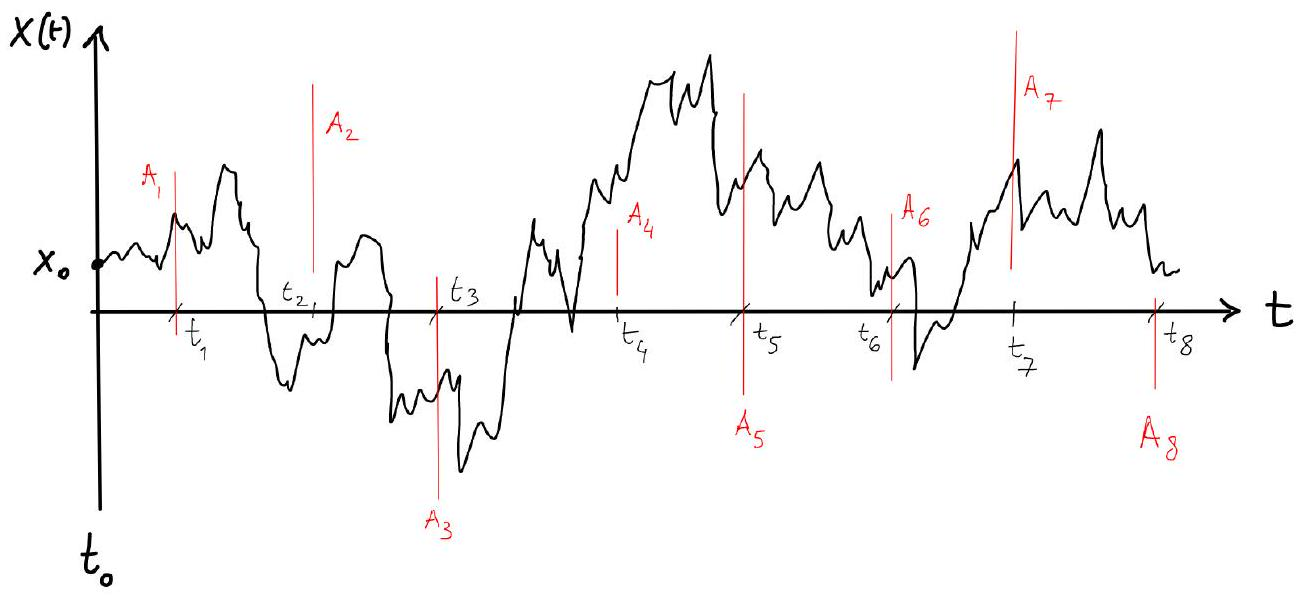
\includegraphics[width=\textwidth]{graphics/2025_10_17_55d6813539323d2293f0g-2}
\end{figure}
The explicit expression is $\left(\Delta t_{i}=t_{i}-t_{i-1}>0\right)$
\begin{DispWithArrows}[displaystyle, format=c]
  d \mathbb{P}_{t_{1} \ldots t_{n}}\left(x_{1} \ldots x_{n} \mid x_{0}, t_{0}\right)=e^{-\frac{1}{2 D} \sum_{i=1}^{n} \frac{\left(x_{i}-x_{i-1}\right)^{2}}{\Delta t_{i}}} \prod_{i=1}^{n} \frac{d x_{i}}{\sqrt{2 \pi D \Delta t_{i}}}
\end{DispWithArrows}
This relation is valid for any $n \in \mathbb{N}$ and we can extend the result
to any subset of the $\sigma$-algebra generated by the cylindrical sets of the
form
$A=\left\{x(t): x\left(t_{1}\right) \in A_{1}, x\left(t_{2}\right) \in A_{2} \ldots x\left(t_{n}\right) \in A_{n}\right\}$.
When we take the limit $n \rightarrow \infty$ we obtain the so called Wiener
path integral. In this case
\begin{DispWithArrows}[displaystyle, format=c]
  \sum_{i=1}^{n} \frac{\left(x_{i}-x_{i-1}\right)^{2}}{\Delta t_{i}}=\sum_{i=1}^{n}\left(\frac{x_{i}-x_{i-1}}{\Delta t_{i}}\right)^{2} \Delta t_{i} \xrightarrow[\substack{n \to \infty \\ \max(\Delta t_i) \to 0}]{\sum \Delta t_i = T} \int_{0}^{T}(\dot{x}(s))^{2} d s
\end{DispWithArrows}
and eq. (16) gets the suggestive form
\begin{DispWithArrows}[displaystyle, format=c]
  d \mathbb{P}_{w} \propto \prod_{\tau=0^{+}}^{T} d x(\tau) e^{-\frac{1}{2 D} \int_{0}^{T} \dot{x}(s)^{2} d s}
\end{DispWithArrows}
This formula is only formal as it does not exist (it is infinite!). However, it
is very useful for calculating averages of functionals which are exponentials
of quadratic expressions of the trajectory $x(s)$ or for approximations with
the saddle point method.
Another way to look at eq. (14b) is the following. We fix $x_{n}=x$, $t_{n}=T$
and $x_{0}$ at $t_{0}$. Then all the integrations
$x_{n-1}, x_{n-2} \ldots, x_{1}$ at the corresponding ordered times
$t_{n-1}, \ldots t_{1}$ show that in the limit $n \rightarrow \infty$ (with
fixed $x, T ; x_{0}, t_{0}$ ) the propagator of a Brownian particle
$W\left(x, T \mid x_{0}, t_{0}\right)$ can be written as
\begin{DispWithArrows}[displaystyle, format=c]
  w\left(x, T \mid x_{0}, t_{0}\right)=\int_{x(0)=x_0}^{x(T)=x} \mathcal{D} x(\tau) e^{-\frac{1}{2 D} \int_{0}^{T} \dot{x}(s)^{2} d s}=\int_{x(0)=x_0}^{x(T)=x} \mathcal{D} x(\tau) e^{-S[x(s)]}
\end{DispWithArrows}
\begin{figure}[H]
  \centering
  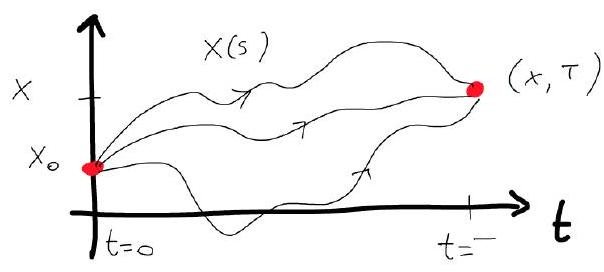
\includegraphics[width=\textwidth]{graphics/2025_10_17_55d6813539323d2293f0g-3}
\end{figure}
the propagator $W$ can be written as an integral over all trajectories between
($t_0, x_{0}$) and ($T, x$) of the Brownian particle.

Here $S[x(s)]$ is the action and $S=\int_{0}^{T} L[x] d s$, where $L$ is the
Lagrangian of the system. Here
$L[x(s)]=\frac{1}{2 D}\left(\frac{d x}{d s}\right)^{2}$ which can be interpreted
as the kinetic energy of a free particle. Furthermore, notice that if we change
variable $s=i t / \hbar$ (as an analytic continuation), identify
$D=\frac{\hbar^{2}}{m}$ and introduce the "imaginary" time $\tilde{t}=-i \hbar T$,
then the propagator in (17b) becomes
\begin{DispWithArrows}[displaystyle, format=c]
  W\left(x, \tilde{t} \mid x_{0}, 0\right)=\int_{x(0)=x_0}^{x(\tilde{t})=x} \mathcal{D} x\left(t^{\prime}\right) e^{\frac{i}{\hbar} \int_{0}^{\tilde{t}} \frac{1}{2} m\left(\frac{d x}{d t^{\prime}}\right)^{2} d t^{\prime}}=\sqrt{\frac{m}{2 \pi i \hbar \tilde{t}}} e^{\frac{i m}{2 \hbar \tilde{t}}\left(x-x_{0}\right)^{2}}
\end{DispWithArrows}
This is the propagator (or Green's function) of the Schrödinger eq:
\begin{DispWithArrows}[displaystyle, format=c]
  i \hbar \frac{\partial \psi}{\partial t}=\hat{H} \psi \quad \text { where } \quad \hat{H}=-\frac{\hbar^{2}}{2 m} \frac{\partial^{2}}{\partial x^{2}}
\end{DispWithArrows}
we can write
$W\left(x, \tilde{t} \mid x_{0}, 0\right)=\\langle x| e^{-\frac{i}{\hbar} \tilde{t} \hat{H}}\left|x_{0}\right\rangle$
and correspondingly we can also write
$\hat{H}|k\rangle=\frac{\hbar^{2}}{2 m} k^{2}|k\rangle=\frac{D k^{2}}{2}|k\rangle$
\begin{DispWithArrows}[displaystyle, format=ll]
  \begin{aligned}
    W\left(x, T \mid x_{0}, 0\right) & =\langle x| e^{-T H}\left|x_{0}\right\rangle=\int d k \int d k^{\prime}\left\langle x \mid k^{\prime}\right\rangle\left\langle k^{\prime}\right| e^{-T H}|k\rangle\langle k \mid x_0\rangle=\\
    = & \frac{1}{2 \pi} \int d k e^{-\frac{D}{2} T k^{2}} e^{i k\left(x-x_{0}\right)}=\frac{1}{\sqrt{2 \pi D T}} e^{-\frac{\left(x-x_{0}\right)^{2}}{2 D T}} \quad\left\langle x \mid k^{\prime}\right\rangle=\frac{1}{\sqrt{2 \pi}} e^{i k^{\prime} x}
  \end{aligned}
\end{DispWithArrows}
This can be generalized to the case of
$\hat{H}=-\frac{\hbar^{2}}{2 m} \frac{\partial^{2}}{\partial x^{2}}+V(x)$
(Schulman, Ch.9). Similar connections to statistical mechanics as
$T \rightarrow \beta$ (Ch. 26).

\subsection*{Two-point correlation function (exercise)}
With the help of eq. (16) it is easy to calculate the 2-point correlation
function which is defined as $\left\langle x\left(t_{1}\right) x\left(t_{2}\right)\right\rangle$
for $t_{0}<t_{1}<t_{2}$. We assume that the particle starts at
$x_{0}=x\left(t_{0}\right)$.
\begin{figure}[H]
  \centering
  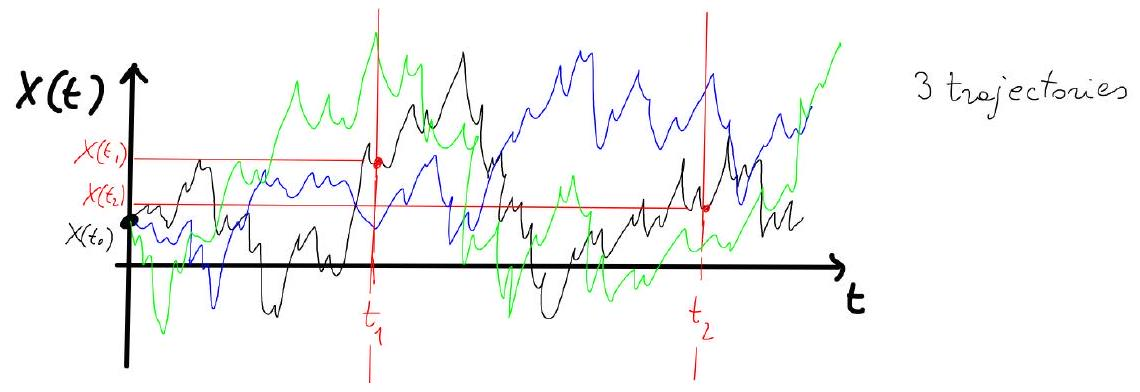
\includegraphics[width=\textwidth]{graphics/2025_10_17_55d6813539323d2293f0g-4}
\end{figure}
Average over Brownian trajectories, all starting at $x_{0}$ at time $t=t_{0}$,
when looking at the trajectories at times $t=t_{1}$ and $t=t_{2}$.
\begin{DispWithArrows}[displaystyle, format=c]
  \left\langle x\left(t_{1}\right) x\left(t_{2}\right)\right\rangle_{w}=\iint d \mathbb{P}_{t_{1} t_{2}}\left(x_{1}, x_{2} \mid x_{0}, t_{0}\right) x_{1} x_{2}
\end{DispWithArrows}
\begin{DispWithArrows}[displaystyle, format=c]
  =\int_{-\infty}^{+\infty} d x_{2} \int_{-\infty}^{+\infty} d x_{1} \frac{1}{\sqrt{2 \pi D\left(t_{2}-t_{1}\right)}} e^{-\frac{1}{2 D} \frac{\left(x_{2}-x_{1}\right)^{2}}{t_{2}-t_{1}}} \frac{1}{\sqrt{2 \pi D\left(t_{1}-t_{0}\right)}} e^{-\frac{1}{2 D} \frac{\left(x_{1}-x_{0}\right)^{2}}{t_{1}-t_{0}}} x_{2} x_{1}
\end{DispWithArrows}
We change variables: $x=x_{1}-x_{0}, y=x_{2}-x_{1}$
\begin{DispWithArrows}[displaystyle, format=c]
  x_{2}=x_{0}+x+y \quad x_{1}=x+x_{0} \quad\left(x_{0} \text { is a const. }\right)
\end{DispWithArrows}
Remember the Jacobian in the transformation:
\begin{DispWithArrows}[displaystyle, format=ll]
  p\left(x_{1}, x_{2}\right) d x_{1} d x_{2}=p\left(x_{1}(x, y), x_{2}(x, y)\right)|J| d x d y \\ J=\begin{pmatrix}
    \frac{\partial x_{1}}{\partial x} & \frac{\partial x_{1}}{\partial y} \\    \frac{\partial x_{2}}{\partial x} & \frac{\partial x_{2}}{\partial y}\end{pmatrix}=\begin{pmatrix}1 & 0 \\ 1 & 1\end{pmatrix} \Rightarrow|J|=1
\end{DispWithArrows}
From eq. (18) we get
\begin{DispWithArrows}[displaystyle, format=ll]
  \begin{aligned}
    & =\int_{-\infty}^{+\infty} d x \int_{-\infty}^{+\infty} d y \frac{1}{\sqrt{2 \pi D\left(t_{2}-t_{1}\right)}} e^{-\frac{1}{2 D} \frac{y^{2}}{t_{2}-t_{1}}} \frac{1}{\sqrt{2 \pi D\left(t_{1}-t_{0}\right)}} e^{-\frac{1}{2 D} \frac{x^{2}}{t_{1}-t_{0}}}\left(x_{0}+x+y\right)\left(x+x_{0}\right) \\
    & =\int_{-\infty}^{+\infty} d x \frac{e^{-\frac{x^{2}}{2 D\left(t_{1}-t_{0}\right)}}}{\sqrt{2 \pi D\left(t_{1}-t_{0}\right)}} (x^2+x_0^2) \\
    & =D\left(t_{1}-t_{0}\right)+x_{0}^{2}
  \end{aligned}
\end{DispWithArrows}
Thus for a generic pair of times $t_{1}, t_{2}>t_{0}$:
\begin{DispWithArrows}[displaystyle, format=c]
  \left\langle x\left(t_{1}\right) x\left(t_{2}\right)\right\rangle_{w}=D \min \left\{t_{1}-t_0, t_{2}-t_0\right\}+x_{0}^{2}
\end{DispWithArrows}
Exercise: calculate
$\left\langle x\left(t_{1}\right) x\left(t_{2}\right)\right\rangle_{w}$ for a
generic initial distribution $g\left(x_{0}\right)$.

\subsection*{Averaging a functional with the Wiener path integral}
Functionals of trajectories (say, position of a particle in time) occur many
times in Physics. For example, one may want to calculate the average of
$F\left(\int_{0}^{T} a(s) x(s) d s\right)$, where $x(s)$ is the value of the
Brownian trajectory at time $s$, $a(s)$ is a smooth function of time and $F$ is
another smooth function.

For any specific calculation we will rely on the discrete, finite $n$, formula
in eq. (16). Namely, if we wish to find the expected value of a functional such
as $F\left(\int_{0}^{T} a(t) x(t) d t\right)$, we first take its discrete
version, $\sum_{i} \Delta t_{i} a\left(t_{i}\right) x\left(t_{i}\right)$, use eq.
(16) for the calculations and only at the end we take the limit
$n \rightarrow \infty, \Delta t \rightarrow 0$.

In the following we will also use the function $A(s)=\int_{s}^{T} a(\tau) d \tau$
which satisfies $\dot{A}(s)=-a(s)$ and $A(T)=0$. Now, $x(0)=0$
\begin{DispWithArrows}[displaystyle, format=c]
  \int_{0}^{T} a(s) x(s) d s=-\left.x(s) \int_{s}^{T} a(\tau) d \tau\right|_{s=0} ^{s=T}+\int_{0}^{T} \dot{x}(s) \left(\int_{s}^{T} a(\tau) d \tau\right) d s=\int_{0}^{T} \dot{x}(s) A(s) d s
\end{DispWithArrows}
This can be written down in the discrete form as
\begin{DispWithArrows}[displaystyle, format=c]
  \int_{0}^{T} A(s) \dot{x}(s) d s=\int_{0}^{x(T)} A(s(x)) d x=\lim _{\substack{n \rightarrow \infty \\ \max _{i}\left(\Delta x_{i}\right) \rightarrow 0}} \sum_{i=1}^{n} A_{i} \underbrace{\left(x_{i}-x_{i-1}\right)}_{\equiv \Delta x_{i}}
\end{DispWithArrows}
From now on we set $2 D=1$ (in the end we replace $t \rightarrow 2 D t$). We use
the Wiener measure in eq. (16) and calculate the average of the discretized
functional $F,\left\langle I_{n}\right\rangle$, for a fixed $n$:
\begin{DispWithArrows}[displaystyle, format=c]
  \left\langle I_{n}\right\rangle=\int_{\mathbb{R}^{n}} \prod_{i=1}^{n} \frac{d x_{i}}{\sqrt{\pi \Delta t_{i}}} F\left(\sum_{i=1}^{n} A_{i} \Delta x_{i}\right) e^{-\sum_{i=1}^{n} \frac{\left(\Delta x_{i}\right)^{2}}{\Delta t_{i}}}
\end{DispWithArrows}
Now we change variables: $y_{i}=\Delta x_{i}$, so
$x_{i}=\sum_{k=1}^{i} y_{k}+x_{0}$ for $i=1,2 \ldots, n$
Remember:
$\quad q(\{y\})=p(\{x(y)\})\left|\frac{\partial x}{\partial y}\right|$

We have to be careful about the jacobian $J$:
\begin{DispWithArrows}[displaystyle, format=c]
  J=\begin{pmatrix}\frac{\partial x_{1}}{\partial y_{1}} & \frac{\partial x_{1}}{\partial y_{2}} & \cdots & \frac{\partial x_{1}}{\partial y_{n}} \\ \vdots & \vdots & \ddots & \vdots \\ \frac{\partial x_{n}}{\partial y_{1}} & \frac{\partial x_{n}}{\partial y_{2}} & \cdots & \frac{\partial x_{n}}{\partial y_{n}}\end{pmatrix}=\begin{pmatrix}1 & 0 & \cdots & 0 \\ 1 & 1 & \cdots & 0 \\ \vdots & \vdots & \ddots & \vdots \\ 1 & 1 & \cdots & 1\end{pmatrix} \Rightarrow \operatorname{det} J=1
\end{DispWithArrows}
hence
\begin{DispWithArrows}[displaystyle, format=c]
  \left\langle I_{n}\right\rangle=\int_{\mathbb{R}^{n}} \prod_{i=1}^{n} \frac{d y_{i}}{\sqrt{\pi \Delta t_{i}}} F\left(\sum_{i} A_{i} y_{i}\right) e^{-\sum_{i} \frac{y_{i}^{2}}{\Delta t_{i}}}
\end{DispWithArrows}
Now we use a little trick. As
$\delta(z)=\frac{1}{2 \pi} \int_{-\infty}^{+\infty} e^{i k z} d k$ and
$F\left(\sum_{i} A_{i} y_{i}\right)=\int F(z) \delta\left(z-\sum_{i} A_{i} y_{i}\right) d z$,
we can write eq. (21) as
\begin{DispWithArrows}[displaystyle, format=ll]
  \begin{aligned}
    \left\langle I_{n}\right\rangle & =\int \prod_{i} \frac{d y_{i}}{\sqrt{\pi \Delta t_{i}}} \int \frac{d k d z}{2 \pi} F(z) e^{i k\left(z-\sum_{j} A_{j} y_{j}\right)} e^{-\sum_{i} \frac{y_{i}^{2}}{\Delta t_{i}}} \\
    & =\int_{-\infty}^{+\infty} \frac{d k d z}{2 \pi} e^{i k z} F(z) \int_{\mathbb{R}^{n}} \prod_{i} \frac{d y_{i}}{\sqrt{\pi \Delta t_{i}}} e^{-\sum_{j}\left(\frac{y_{j}^{2}}{\Delta t_{j}}+i A_{j} y_{j} k\right)} \\
    & =\int_{-\infty}^{+\infty} \frac{d k d z}{2 \pi} e^{i k z} F(z) e^{-\frac{k^{2}}{4} \sum_{i} A_{i}^{2} \Delta t_{i}}=\int d z F(z) \int \frac{d k}{2 \pi} e^{-\frac{k^{2}}{4} \sum_{i} A_{i}^{2} \Delta t_{i}+i k z} \\
    & =\int d z F(z) \frac{e^{-\frac{z^{2}}{\sum_{i} A_{i}^{2} \Delta t_{i}}}}{\left(\pi \sum_{i} A_{i}^{2} \Delta t_{i}\right)^{1 / 2}}=\int_{-\infty}^{+\infty} d z F(z) N_{z}\left(0, \frac{1}{2}\sum_{i} A_{i}^{2} \Delta t_{i}\right)
  \end{aligned}
\end{DispWithArrows}
Hence
\begin{DispWithArrows}[displaystyle, format=c]
  \left\langle F\left(\sum_{i} A_{i} \Delta x_{i}\right)\right\rangle_{BM}=\int_{-\infty}^{+\infty} d z F(z) N_{z}(0, \frac{1}{2}\sum_{i} A_{i}^{2} \Delta t_{i})
\end{DispWithArrows}
Where $N_{z}\left(\mu, \sigma^{2}\right)$ is the Normal distribution with mean
$\mu$ and variance $\sigma^{2}$. We can now take the limit
$n \rightarrow \infty, \Delta t_{i} \rightarrow 0$:
\begin{DispWithArrows}[displaystyle, format=c]
  \sum_{i} A_{i}^{2} \Delta t_{i} \longrightarrow \int_{0}^{T} A^{2}(s) d s=\int_{0}^{T}\left(\int_{s}^{T} a(\tau) d \tau\right)^{2} d s \equiv R(T)
\end{DispWithArrows}
Thus the continuum formulation gives:
\begin{DispWithArrows}[displaystyle, format=c]
  \left\langle F\left(\int_{0}^{T} a(s) x(s) d s\right)\right\rangle_{BM}=\int_{-\infty}^{+\infty} d z F(z) N_{z}(0, D R(T))
\end{DispWithArrows}
where $R(T)$ is defined in (23). If we introduce $2D$, we get
\begin{DispWithArrows}[displaystyle, format=c]
  N_{z}(0, 2DR(T))=\frac{1}{\sqrt{4 \pi D R(T)}} e^{-\frac{z^{2}}{4 D R(T)}}
\end{DispWithArrows}
Example:
If $F(z)=e^{h z}$ we obtain the moment generating function of
$\int_{0}^{T} a(s) x(s) d s$, namely
\begin{DispWithArrows}[displaystyle, format=c]
  \left\langle e^{h \int_{0}^{T} a(s) x(s) d s}\right\rangle_{BM}=e^{D R(T) h^{2}}
\end{DispWithArrows}
Exercise: Take $F(z)=e^{z}, a(s)=h_{1} \delta\left(t_{1}-s\right)+h_{2} \delta\left(t_{2}-s\right)$
for $0<t_{1}, t_{2}<T$. Calculate $A(s)$ and $R(T)$. Since
$\int_{0}^{T} a(s) x(s) d s=h_{1} x\left(t_{1}\right)+h_{2} x\left(t_{2}\right)$,
calculate
$z\left(h_{1}, h_{2}\right)=\left\langle e^{h_{1} x\left(t_{1}\right)+h_{2} x\left(t_{2}\right)}\right\rangle_{w}$
and finally show that
\begin{DispWithArrows}[displaystyle, format=c]
  \left.\frac{\partial^{2} z}{\partial h_{1} \partial h_{2}}\right|_{h_{1}=0=h_{2}}=\left\langle x\left(t_{1}\right) x\left(t_{2}\right)\right\rangle_{BM}=2D \min \left\{t_{1}, t_{2}\right\}
\end{DispWithArrows}

\subsection*{A brief summary of what we have done:}
We have learnt some properties of the Brownian process:
\begin{enumerate}
  \item It is the most important continuous stochastic process, which is tightly
    linked to the diffusion equation. It is a Markov process with continuous
    paths, but very irregular ones as it is nowhere differentiable.
  \item We know how to simulate it.
  \item It can be used to define a path integral, an object that is not very
    well defined but (at least in its discrete form) it can be used to calculate
    some functionals that are useful in Physics and beyond.
\end{enumerate}

At this point we want to use the Brownian motion to build up new continuous
stochastic processes. We will do that by defining stochastic differential
equations (SDEs). This needs a lot of care because there are many subtleties
with continuous stochastic processes. We will look into the main features. There
are many books which develop SDEs rigorously.

% Lecture file created by newnote
% Class: Models of Theoretical Physics
% Professor: Azaele Sandro
% Date: 2025-10-17
\lecture{8}{Introduction to Stochastic Processes}{2025-10-17}
\pagelayout{margin}
% --- Start writing here ---

\section{Introduction to Stochastic Processes}
We will present basic results from the theory of stochastic processes. Rigorous definitions and proofs need notions of measure theory that we do not introduce nor assume. therefore, this introduction will necessarily be non-rigorous, with some looseness in the definitions and some inaccuracies in the proofs. There are many books which can give you the mathematical rigor that is necessary for obtaining a full understanding of stochastic processes. These notes, instead, wish to provide enough awareness to make you able to use the tools in applied problems (in physics, biology, finance...).

In the following we will connect the diffusion equation to the most important continuous stochastic process: the Brownian motion (or Wiener Process). This is the basis for building up stochastic differential equations whose solutions have continuous trajectories. These are crucial for defining stochastic models that will be used in several fields of physics.

Useful books:
\begin{itemize}
    \item "Intro. to Stoch. Calculus with Applic.", F.C. Klebaner, Imperial P.
    \item "An Introd. to SDEs", Lawrence C. Evans, AMS
    \item "Stoch. Proc. and Applications", G. A. Pavliotis, Springer
    \item "Stoch. Methods", C. Gardiner, Springer
    \item "Stoch. Diff. Eq.", B. Oksendal, Springer
    \item "Stoch. proc. in Physics and chemistry", N.G. van Kampen.
\end{itemize}

\subsection*{Example: Tossing a coin}
Let's assume that we toss a coin 3 times (heads $\rightarrow 0$, tails $\rightarrow 1$) and we ask: what is the sum of the 3 tosses? We define a function from the sample space (the realization) to the state space (what we measure)
$Y: \Omega=\{\omega_1=(0,0,0), \omega_2=(0,0,1) \ldots \omega_8=(1,1,1)\} \longrightarrow E=\{y_1=0, y_2=1, y_3=2, y_4=3\}$
and introduce probabilities $\mathbb{P}: \Omega \rightarrow[0,1]$ s.t. $\sum_{\omega} P(\omega)=1$; we define $P_{i}=\sum_{\omega: Y(\omega)=y_{i}} \mathbb{P}(\omega)=P\left(Y=y_{i}\right)$. More generally, we can define probabilities for all sets of type $Y^{-1}(B) \subseteq \Omega$, for $B \subseteq E$. This means that $Y$ is a measurable function and this defines a random variable.
When $\Omega$ is finite, $Y(\Omega)$ is finite and we can always define a random variable as before. We can also define the expectation as
\begin{DispWithArrows}
    E(Y)=\sum_{\omega \in \Omega} Y(\omega) \mathbb{P}(\omega)=\sum_{i=1}^{4} y_{i} P\left(Y=y_{i}\right)=\sum_{i=1}^{4} y_{i} P_{i}
\end{DispWithArrows}
When $\Omega$ is an uncountable set, the definition of r.v. needs much care, because we have to make sure that $x$ is still a measurable function. In simple terms $x$ is a real-valued random variable when we can assign probabilities to sets (called events) of the form {x \leq c} and {a<x \leq b} for $x, a, b \in \mathbb{R}$.
\begin{figure}[H]
    \centering
    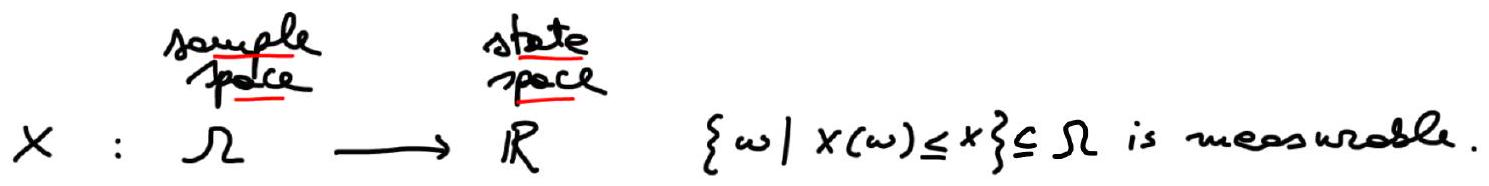
\includegraphics[width=0.5\textwidth]{2025_10_17_79731b7d4e7690819b81g-02}
\end{figure}
More precisely, a random variable is a measurable function for which the preimage of any Borel set in $\mathbb{R}$ is a measurable set in $\Omega$.

\subsection*{Definition of stochastic process}
A stochastic process is a collection of random variables {x(t, $\omega$), t \in T, $\omega$ \in $\Omega$}, where T is an ordered set ("time") (it can be either discrete, $T=\mathbb{Z}_{+}$, or continuous, $T=\mathbb{R}^{+}$). For each fixed time $t \in T, x(t, \omega)$ indicates a random variable from $\Omega$ (rigorously, from the probability space $(\Omega, \mathcal{F}, \mathbb{P})$ ) to $E$ (rigorously, $E$ is a measurable space equipped with a $\sigma$-algebra; for instance, $E=\mathbb{R}^{d}$ and the $\sigma$-algebra is the one of Borel sets; we need a "filtration" as well).
$\Omega$ is the common sample space, $E$ is the state space of the process.
For each fixed $\omega \in \Omega, x(t, \omega)$ is a function of time $t$ that is called a sample path or a stochastic realization of the process. We will usually omit the $\omega$-dependence, i.e., we write $x(t)$.

\subsection*{Examples:}
\begin{enumerate}
    \item Let $E=\{0,1,-1\}$ be the state space of a stoch-proc $x$ and let $T=\{0,1,2,3\}$ be the (discrete) time. There are then $3^{4}$ sample paths, thus $|
\Omega|=3^{4}=81$.
    \begin{figure}[H]
        \centering
        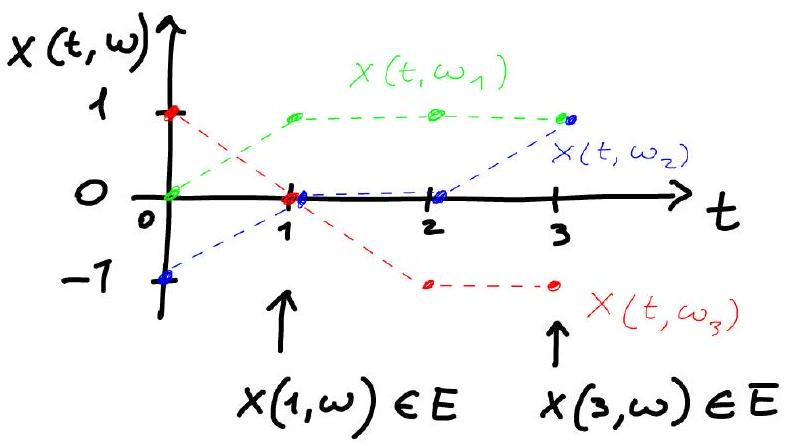
\includegraphics[width=0.5\textwidth]{2025_10_17_79731b7d4e7690819b81g-03}
    \end{figure}
    In this example we can enumerate all the 81 trajectories. This is not possible if $E$ is an uncountable set.
    \item The random walk process in discrete time has $E=\mathbb{Z}$ (position) and $T=\mathbb{N}$ (time), thus $x(t, \omega)$ indicates a stochastic realization (or trajectory) as a function of time $t$.
    \begin{figure}[H]
        \centering
        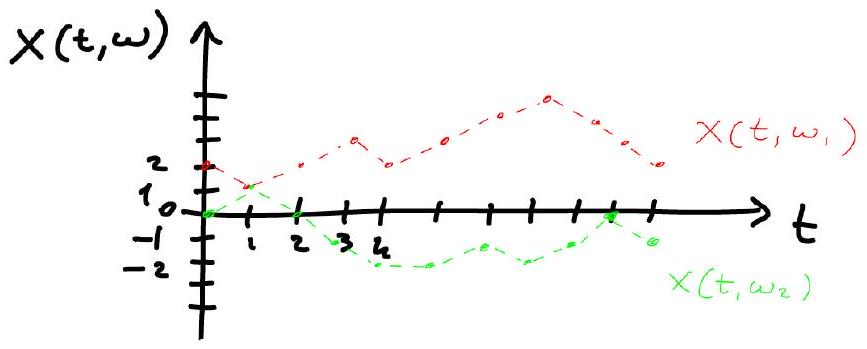
\includegraphics[width=0.5\textwidth]{2025_10_17_79731b7d4e7690819b81g-03(1)}
    \end{figure}
    Here we get infinitely countable trajectories ($|
\Omega|=|\mathbb{Z}|^{\mathbb{N}}$)
    \item The position of a Brownian particle is described by the Brownian process for which $T=\mathbb{R}^{+}$ and $E=\mathbb{R}$ and one sample path is $x(t, \omega)$
    \begin{figure}[H]
        \centering
        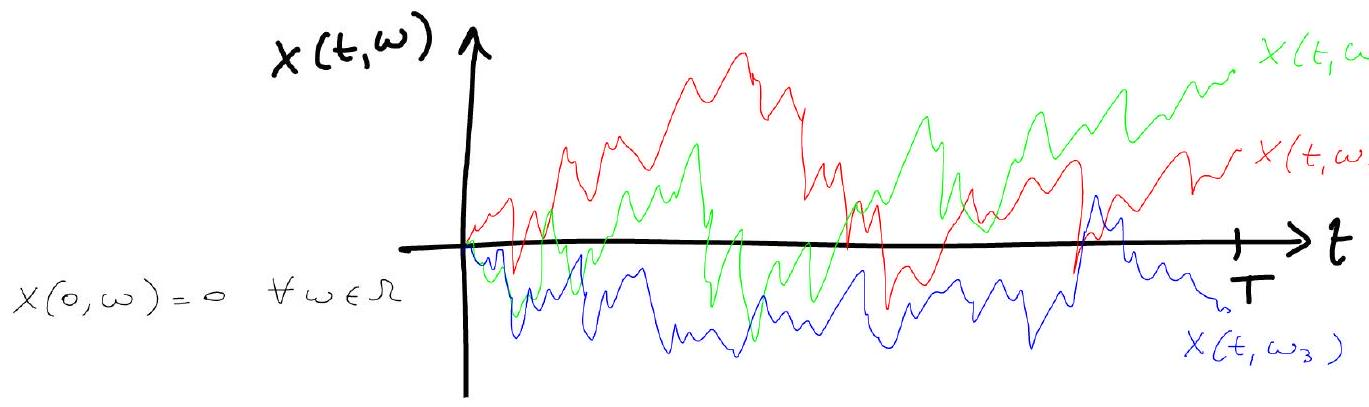
\includegraphics[width=0.5\textwidth]{2025_10_17_79731b7d4e7690819b81g-03(2)}
    \end{figure}
    here every path is a continuous function of time $x(t, \omega) \in C^{0}([0, T])$
\end{enumerate}
In the following we will omit $\omega$ and we will simply write $x(t)$, because what we "observe" is the value $x \in E$ at some time $t$ and not $
\Omega$.

Notice that in these examples we have not defined a prob. measure, which is not needed for defining a random variable.

One of the most important stochastic processes is the Brownian process/motion or Wiener process.
This can be used to describe the motion of a heavy particle in a fluid made of light particles, which collide with it randomly. For the time being, we will not look into how good this process is for empirical Brownian particles.

\subsection*{Brownian motion (or Wiener process)}
A standard Brownian motion in 1-d, $B(t)$, is a real-valued stoch. process ($E=\mathbb{R}, T=\mathbb{R}^{+}$) for which
(A) $B(0)=0$ (a.s. , namely, Prob. {B(0)=0}=1)
(B) For any $0 \leqslant s<t<\infty, B(t)-B(s)$ is normally distributed, that is $B(t)-B(s) \sim N(0, t-s)=\frac{1}{\sqrt{2 \pi(t-s)}} e^{-\frac{\Delta x^{2}}{2(t-s)}}$ (mean 0 and variance $t-s$)
(C) For all times $0=t_{0}<t_{1}<t_{2}<\ldots<t_{n}$ the increments $\Delta B_{i}:=B\left(t_{i}
ight)-B\left(t_{i-1}
ight)$ are independent (of each other)

Some important properties:
\begin{enumerate}
    \item Stationarity of increments: notice that, if we write $t=s+\Delta t$, then from (B) we get
    \begin{DispWithArrows}
        B(s+\Delta t)-B(s) \sim N(0, \Delta t)
    \end{DispWithArrows}
    which means that the distribution of $B(s+\Delta t)-B(s)$ does not depend on $s$. This means that the increments are not only independent, but also stationary, namely they depend only on $\Delta t: \Delta B=B(s+\Delta t)-B(s) \sim B(\Delta t)$.

    Since $\operatorname{Var}[B(\Delta t)]=\Delta t$, we expect that $|
\Delta B|=|B(\Delta t)| \simeq \sqrt{\Delta t}$ as $\Delta t \rightarrow 0^{+}$. This will be crucial in the future, in many calculations.
    \item Connection with the diffusion equation

    We have seen that the fundamental solution of the diffusion eq. ($D=1$)
    \begin{DispWithArrows}
        \left\{\begin{array}{cc}
        \partial_{t} w(x, t)=\frac{1}{2} \partial_{x}^{2} w(x, t) & x \in \mathbb{R}, t>t_{0} \\
        w(x, t_{0})=\delta\left(x-x_{0}
ight) & t=t_{0}
        \end{array}\right.
    \end{DispWithArrows}
    is the propagator of the Brownian motion:
    \begin{DispWithArrows}[tag=1]
        w\left(x, t \mid x_{0}, t_{0}
ight)=\frac{1}{\sqrt{2 \pi\left(t-t_{0}
ight)}} e^{-\frac{\left(x-x_{0}
ight)^{2}}{2\left(t-t_{0}
ight)}}
    \end{DispWithArrows}
    which is the one we use in (B). So from time to time the process evolves with the propagator (1) and with stationary independent increments.
    \item Correlation function

    The average will be indicated either with $\langle\cdots\rangle$ or with $\mathbb{E}(\cdots)$. Let $0 \leqslant s \leqslant t:$ from (B) $\mathbb{E}[B(s)]=0, \mathbb{E}\left[B(s)^{2}
ight]=s$. Then
    \begin{DispWithArrows}
        \begin{aligned}
        \mathbb{E}[B(t) B(s)] & =\mathbb{E}[(B(s)+B(t)-B(s)) B(s)]=\
        & =\mathbb{E}\left[B(s)^{2}+(B(t)-B(s)) B(s)\right]=\
        & =\mathbb{E}\left[B(s)^{2}\right]+\mathbb{E}[(B(t)-B(s)) B(s)]=\
        & =s+\mathbb{E}[(B(t)-B(s))] \mathbb{E}[B(s)]=s
        \end{aligned}
    \end{DispWithArrows}
    Thus for $s, t \geqslant 0$
    \begin{DispWithArrows}[tag=2]
        \mathbb{E}[B(t) B(s)]=\min (t, s)
    \end{DispWithArrows}
    Exercises:
    i) (Ornstein-Uhlenbeck process). Define $V(t)=e^{-t} B\left(e^{2 t}
ight)$ where $B(t)$ is a Brownian process. Show that $\mathbb{E}[V(t)]=0$ and $\mathbb{E}[V(t) V(s)]=e^{-|t-s|}$.
    ii) (Brownian bridge). Define $V(t)=B(t) - (t/T)B(T)$ for any $t \in[0, T]$, where $B(t)$ is a Brownian process. Show that $\mathbb{E}[V(t)]=0$ and $\mathbb{E}[V(t) V(s)]=\min(t,s) - ts/T$ for any $t, s \in[0, T]$.
    iii) Show that $\mathbb{E}\left[e^{i \lambda B(t)}\right]=e^{-\frac{\lambda^{2} t}{2}}$ for $t \geqslant 0, B(t)$ B.m.
    iv) With the help of the Law of large numbers and $B(t)=\sum_{i=1}^{t/\Delta t} \Delta B_{i}$, show that $\lim _{t \rightarrow \infty} \frac{B(t)}{t}=0$.
    \item Rescaling. The process $z(t)=\frac{1}{\sqrt{c}} B(c t), c>0$, is a Brownian motion that is distributed like $B(t)$, another Brownian motion. (Verify $(A),(B)$ and $(C)$ ). Also:
    \begin{DispWithArrows}
        \mathbb{E}\left[e^{i \lambda z(t)}\right]=\mathbb{E}\left[e^{i \lambda \frac{1}{\sqrt{c}} B(c t)}\right]=e^{-\frac{\lambda^{2}}{2 c} t c}=e^{-\frac{\lambda^{2} t}{2}}=\mathbb{E}\left[e^{i \lambda B(t)}\right]
    \end{DispWithArrows}
    \item Inversion. The process $z(t)=t B\left(\frac{1}{t}
ight)$ for $t>0$ and $z(0)=0$ is distributed like $B(t)$, another B.m.
    \begin{DispWithArrows}
        \mathbb{E}\left[e^{i \lambda z(t)}\right]=\mathbb{E}\left[e^{i \lambda t B\left(\frac{1}{t}
ight)}\right]=e^{-\frac{\lambda^{2}}{2} t^{2} \cdot \frac{1}{t}}=e^{-\frac{\lambda^{2} t}{2}}=\mathbb{E}\left[e^{i \lambda B(t)}\right]
    \end{DispWithArrows}
    Notice that $\lim _{t \to \infty} \frac{z(t)}{t}=\lim _{t \to \infty} B\left(\frac{1}{t}
ight)=0$ as in (iv).
    \item Time reversal. Define $z(t)=B(T)-B(T-t)$ for any $t \in[0, T]$. Then $Z(t)$ and $B(t)$ have the same distrib.
\end{enumerate}

\subsection*{Properties of the trajectories of the Brownian motion}
These are hard to prove rigorously, but somehow easy to guess. Let's consider the ratio $rac{\Delta B}{(\Delta t)^{\alpha}}$ where $\Delta t=t_{2}-t_{1}>0, \alpha>0$ and $\Delta B=B\left(t_{2}
ight)-B\left(t_{1}
ight)$. What happens to this ratio as $\Delta t \rightarrow 0^{+}$? Take some $k \in \mathbb{R}^{+}$:
\begin{DispWithArrows}[tag=3]
    \begin{aligned}
    P\left(\left|\frac{\Delta B}{\Delta t^{\alpha}}\right| \leqslant k\right) & =P\left(|
\Delta B| \leqslant k \Delta t^{\alpha}\right)=\int_{-k(\Delta t)^{\alpha}}^{k(\Delta t)^{\alpha}} d x \frac{e^{-\frac{x^{2}}{2 \Delta t}}}{\sqrt{2 \pi \Delta t}}}=\
    & =\frac{2}{\sqrt{2 \pi \Delta t}} \int_{0}^{k(\Delta t)^{\alpha}} d x e^{-\frac{x^{2}}{2 \Delta t}}=\frac{2}{\sqrt{2 \pi}} \int_{0}^{k(\Delta t)^{\alpha-1 / 2}} d z e^{-z^{2} / 2}
    \end{aligned}
\end{DispWithArrows}
Here are the consequences:
\begin{enumerate}
    \item $0<\alpha<\frac{1}{2}$, as $\Delta t \rightarrow 0^{+}, \quad P\left(\left|\frac{\Delta B}{\Delta t^{\alpha}}\right| \leqslant k\right) \rightarrow 1$ regardless of $k$. This tells us that as $|t-s| \rightarrow 0^{+}$
    \begin{DispWithArrows}
        $|B(t)-B(s)| \leqslant \text { const }|t-s|^{\alpha}$
    \end{DispWithArrows}
    which means that Brownian trajectories are Hölder continuous for any $0<\alpha<\frac{1}{2}$. This can be proven rigorously.
    \item $\alpha=1$ (or $\frac{1}{2}<\alpha \leqslant 1$), as $\Delta t \rightarrow 0^{+}, P\left(\left|\frac{\Delta B}{\Delta t}\right| \leqslant k\right) \rightarrow 0 \quad \forall k \in \mathbb{R}^{+}$
\end{enumerate}
This tells us that the Brownian trajectories are nowhere differentiable. This is expected because if $|
\Delta B| \sim \sqrt{\Delta t}$, then $\frac{|
\Delta B|}{\Delta t} \sim \frac{1}{\sqrt{\Delta t}}$ and hence $\lim _{\Delta t \rightarrow 0^{+}} \frac{|
\Delta B|}{\Delta t} \rightarrow \infty$.
This is related to the fact that B.m. has no memory of the past (see the Markov property below).

We can add a drift $\mu$ and change the diffusion coefficient of a Brownian motion with no difficulty. We define a Brownian motion with drift $\mu$ and variance $D$ the process
\begin{DispWithArrows}[tag=4]
    x(t)=x_{0}+\mu t+\sqrt{2D} B(t)
\end{DispWithArrows}
Verify that $\mathbb{E}[x(t)]=x_{0}+\mu t$ and $\operatorname{Var}[x(t)] \equiv \mathbb{E}\left[(x(t)-\mathbb{E}[x(t)])^{2}\right]=2Dt$. Notice that $x(t)$ satisfies the stochastic differential equation:
\begin{DispWithArrows}[tag=5]
    d x(t)=\mu d t+\sqrt{2D} d B(t)
\end{DispWithArrows}
How to simulate a very simple SDE (including B.m.) We wish to generate a path of eq. (5), starting from $x(0)=x_{0}$. Because $\Delta B \sim B(\Delta t) \sim \sqrt{\Delta t} B(1)$ for finite times $t_{0}=0<t_{1} \cdots <t_{n-1}<t_{n}$ we can write (5) as ($\Delta t=t_{i}-t_{i-1}$)
\begin{DispWithArrows}[tag=6]
    \begin{aligned}
    x\left(t_{i}\right) & =x\left(t_{i-1}
ight)+\mu \Delta t+\sqrt{2D \Delta t} \varepsilon_{i} \\
    x(0) & =x_{0}
    \end{aligned} \quad i=1,2, \ldots, n
\end{DispWithArrows}
where $\varepsilon_{i} \sim N(0,1)$. Notice that we use a sequence of $n$ independent and identically distributed random variables {$\varepsilon_{i}$} drawn from $N(0,1)$ because at every time step we add a random value that is independent of all values that were calculated before (indep. of $x, t, \mu, D \ldots$). Of course, $\mu=0, D=1/2$ and $x_{0}=0$ generate a standard Brownian motion as defined in $(A),(B)$ and $(C)$.

\subsection*{Markov processes}
Let us focus on a stochastic process for which we can take a set of ordered times, i.e. $t_{0}<t_{1}<t_{2} \cdots<t_{n}$ and there exists a conditional prob. density funct. at time $t_{n}$, namely $p_{1|n-1}
\left(x_{n}, t_{n} 
\mid x_{n-1}, t_{n-1} ; \ldots ; x_{1}, t_{1} ; x_{0}, t_{0}
ight)$.
This PDF tells us what is the prob. of observing $x_{n}$ at time $t_{n}$, if we know what happened to the process at previous times; we really know the actual values that occurred, not only their probabilities. This is quite a lot of information and basically it means that, if we want to make a prediction on what is going to happen in the future, we have to know all that happened in the past. However, in some situations the effect of the past can be neglected. In particular, if it happens that for any $n=1,2 \ldots$
\begin{DispWithArrows}[tag=7]
    $p_{1|n-1}
\left(x_{n}, t_{n} 
\mid x_{n-1}, t_{n-1} ; \ldots ; x_{1}, t_{1} ; x_{0}, t_{0}
ight)=p_{1|1}
\left(x_{n}, t_{n} 
\mid x_{n-1}, t_{n-1}
ight)$
\end{DispWithArrows}
Then we say that the stochastic process is a Markov process. This means that predictions at time $t_{n}$ only depend on what happened at time $t_{n-1}$ and not on the whole history of the process. The pdf $p_{1|1}$ is called transition probability or propagator.

A Markov process can be fully defined by two functions: the propagator $p_{1|1}$ and the initial distribution $p_{1}
\left(x_{0}, t_{0}
ight)$.

Indeed the 3-point joint PDF for a Markov process is ($t_{0}<t_{1}<t_{2}$):
\begin{DispWithArrows}[tag=8]
    \begin{aligned}
    P_{3}
\left(x_{2} t_{2} ; x_{1} t_{1} ; x_{0} t_{0}
ight) & =P_{1|2}
\left(x_{2} t_{2} 
\mid x_{1} t_{1} ; x_{0} t_{0}
ight) P_{2}
\left(x_{1} t_{1} ; x_{0} t_{0}
ight)=\
    & =p_{1|1}
\left(x_{2} t_{2} 
\mid x_{1} t_{1}
ight) P_{2}
\left(x_{1} t_{1} ; x_{0} t_{0}
ight) \\
    & =P_{1|1}
\left(x_{2} t_{2} 
\mid x_{1} t_{1}
ight) P_{1|1}
\left(x_{1} t_{1} 
\mid x_{0} t_{0}
ight) P_{1}
\left(x_{0} t_{0}
ight)
    \end{aligned}
\end{DispWithArrows}
Therefore we can find iteratively
\begin{DispWithArrows}[tag=9]
    p_{n}
\left(x_{n} t_{n} ; x_{n-1} t_{n-1} ; \ldots ; x_{1} t_{1} ; x_{0} t_{0}
ight)=\prod_{i=1}^{n} p_{1|1}
\left(x_{i} t_{i} 
\mid x_{i-1} t_{i-1}
ight) p_{1}
\left(x_{0} t_{0}
ight)
\end{DispWithArrows}
this property makes Markov processes much more amenable to analytical calculations than non-Markov ones.

\subsection*{The Chapman-Kolmogorov equation}
Not all functions can be used as propagators for Markov processes, nor an initial distribution $p_{1}$ can be arbitrary. These two functions must satisfy two identities, one of which is the C-K. equation.

From the L.H.S. of eq. (8), if we integrate wrt $x_1$,
\begin{DispWithArrows}
    $\int d x_{1} p_{3}
\left(x_{2} t_{2} ; x_{1} t_{1} ; x_{0} t_{0}
ight)=p_{2}
\left(x_{2} t_{2} ; x_{0} t_{0}
ight)$
\end{DispWithArrows}
from the R.H.S., instead
\begin{DispWithArrows}
    $=\int d x_{1} p_{1|1}
\left(x_{2} t_{2} 
\mid x_{1} t_{1}
ight) p_{1|1}
\left(x_{1} t_{1} 
\mid x_{0} t_{0}
ight) p_{1}
\left(x_{0} t_{0}
ight)$
\end{DispWithArrows}
but $p_{2}
\left(x_{2} t_{2} ; x_{0} t_{0}
ight)=p_{1|1}
\left(x_{2} t_{2} 
\mid x_{0} t_{0}
ight) p_{1}
\left(x_{0} t_{0}
ight)$, because of the Markov property, so
\begin{DispWithArrows}[tag=10]
    $p_{1|1}
\left(x_{2} t_{2} 
\mid x_{0} t_{0}
ight) p_{1}
\left(x_{0} t_{0}
ight)=\int d x_{1} p_{1|1}
\left(x_{2} t_{2} 
\mid x_{1} t_{1}
ight) p_{1|1}
\left(x_{1} t_{1} 
\mid x_{0} t_{0}
ight) p_{1}
\left(x_{0} t_{0}
ight)$
\end{DispWithArrows}
hence, for any $t_{2}>t_{1}>t_{0}$
\begin{DispWithArrows}[tag=11]
    $p_{1|1}
\left(x_{2} t_{2} 
\mid x_{0} t_{0}
ight)=\int d x_{1} p_{1|1}
\left(x_{2} t_{2} 
\mid x_{1} t_{1}
ight) p_{1|1}
\left(x_{1} t_{1} 
\mid x_{0} t_{0}
ight)$
\end{DispWithArrows}
this is the Chapman-Kolmogorov equation (actually, identity), which must be satisfied by any propagator/transition probab. If we further integrate eq. (10) w.r.t. $x_{0}$ we get
\begin{DispWithArrows}
    $\int d x_{0} p_{1|1}
\left(x_{2} t_{2} 
\mid x_{0} t_{0}
ight) p_{1}
\left(x_{0} t_{0}
ight)=p_{1}
\left(x_{2} t_{2}
ight)$
\end{DispWithArrows}
and
\begin{DispWithArrows}
    $\int d x_{0} p_{1|1}
\left(x_{1} t_{1} 
\mid x_{0} t_{0}
ight) p_{1}
\left(x_{0} t_{0}
ight)=p_{1}
\left(x_{1} t_{1}
ight)$
\end{DispWithArrows}
we obtain, for $t_{2}>t_{1}$,
\begin{DispWithArrows}[tag=12]
    $p_{1}
\left(x_{2} t_{2}
ight)=\int d x_{1} p_{1|1}
\left(x_{2} t_{2} 
\mid x_{1} t_{1}
ight) p_{1}
\left(x_{1} t_{1}
ight)$
\end{DispWithArrows}
this is the $2^{\text {nd }}$ eq. (identity) for a Markov process. Therefore $p_{1}$ and $p_{1|1}$ are connected to each other.
It can be proven that any two non-negative functions that satisfy eqs. (11) and (12) define a Markov process.

\subsection*{Stationary Markov Process}
If $p_{1}$ is independent of time and equal to the equilibrium distribution of the stochastic process, and $p_{1|1}$ depends only on the time difference $\left|t_{2}-t_{1}
ight|$, then the process is a stationary Markov process.

The Brownian motion is a Markov process
This property essentially follows from the independence of the increments and it can be proven in different ways. In our context, we can use eq. (1), i.e. the propagator
\begin{DispWithArrows}[tag=13]
    $P_{1|1}
\left(x_{1}, t_{1} 
\mid x_{0}, t_{0}
ight) \equiv W\left(x_{1}, t_{1} 
\mid x_{0}, t_{0}
ight)=\frac{1}{\sqrt{2 \pi D\left(t_{1}-t_{0}
ight)}} e^{-\frac{\left(x_{1}-x_{0}
ight)^{2}}{2D\left(t_{1}-t_{0}
ight)}}$
\end{DispWithArrows}
and show that eq. (11) is satisfied by direct integration. Also, if you take $P_{1}
\left(y_{1}, t_{1}=0
ight)=\delta\left(y_{1}
ight)$ you get from eq. (12) $p_{1}
\left(y_{2}, t_{2}
ight)=\frac{1}{\sqrt{2 \pi D t_{2}}} e^{-y_{2}^{2} / 2D t_{2}}$. These generate a non-stationary Markov process.

\subsection*{Exercises:}
\begin{enumerate}
    \item Show that the Poisson process defined by
    \begin{DispWithArrows}
        $P_{1|1}
\left(x_{2} t_{2} 
\mid x_{1} t_{1}
ight)=\frac{\left(\lambda\left(t_{2}-t_{1}
ight)
ight)^{x_{2}-x_{1}}}{\left(x_{2}-x_{1}
ight)!} e^{-\lambda\left(t_{2}-t_{1}
ight)} \quad t_{2}>t_{1}$
    \end{DispWithArrows}
    and $P_{1}(n, 0)=\delta_{n, 0} \Rightarrow P_{1}(n, t)=\frac{(\lambda t)^{n}}{n!} e^{-\lambda t}$ is a (non-stationary) Markov process.
    \item Show that for $x, y= \pm 1$ the function
    \begin{DispWithArrows}
        $P_{1|1}
\left(x t 
\mid y t^{\prime}
ight)=\frac{1}{2}
\left[1+e^{-2 \gamma\left(t-t^{\prime}
ight)}\right] \delta_{x y}+\frac{1}{2}
\left[1-e^{-2 \gamma\left(t-t^{\prime}
ight)}\right] \delta_{x,-y}$
    \end{DispWithArrows}
    satisfies eq. (11).
    \item Show that the process defined by
    \begin{DispWithArrows}
        $P_{1}(x)=\frac{1}{\sqrt{2 \pi}} e^{-x^{2} / 2}$
    \end{DispWithArrows}
    $p_{1|1}
\left(x t 
\mid y, t^{\prime}
ight)=\frac{1}{\sqrt{2 \pi\left(1-e^{-2\left|t-t^{\prime}
ight|}
ight)}} \exp
\left[-\frac{\left(x-y e^{-\left|t-t^{\prime}
ight|}
ight)^{2}}{2\left(1-e^{-2\left|t-t^{\prime}
ight|}
ight)}\right]$ is a stationary Markov process. This is called the O.U. proc.
\end{enumerate}

% !TeX encoding = UTF-8
% Lecture file created by newnote
% Class: Models of Theoretical Physics
% Professor: Azaele Sandro
% Date: 2025-10-17
\lecture{9}{Wick's theorem}{2025-10-17}
\pagelayout{margin}
% --- Start writing here ---

\section{Wick's theorem}
Note that, because of symmetry, the s-point correlation for $s$ any odd integer
is zero (the Gaussian remains unchanged if $\vec{x} \rightarrow-\vec{x}$). 

What happens when we want to calculate
$\left\langle x_{i} x_{j} \cdots x_{l}\right\rangle$? Should we always do all
the derivatives as in eq. (12)? No!
If the vars are Gaussian we can use

\subsection*{Wick's theorem}
Any correlation between an even number of Gaussian r.v. can be written down as
a sum of products of 2-point correlation functions $\left(A^{-1}\right)$.
For instance
\begin{DispWithArrows}[displaystyle, format=ll]
  \begin{aligned}
    \left\langle x_{a} x_{b} x_{c} x_{d}\right\rangle= & \left\langle x_{a} x_{b}\right\rangle\left\langle x_{c} x_{d}\right\rangle+\left\langle x_{a} x_{c}\right\rangle\left\langle x_{b} x_{d}\right\rangle+\left\langle x_{a} x_{d}\right\rangle\left\langle x_{b} x_{c}\right\rangle \\
    & \left(A^{-1}\right)_{a b} \quad \left(A^{-1}\right)_{c d} \quad \cdots \quad \text { (indexes may be equal) }
  \end{aligned}
\end{DispWithArrows}
Exercise: from the previous case, show that (no calculations!)
\begin{DispWithArrows}[displaystyle, format=ll]
  \begin{aligned}
    & \left\langle x_{1}^{2} x_{2}^{2}\right\rangle=\left\langle x_1 x_1\right\rangle \left\langle x_2 x_2\right\rangle + 2\left\langle x_1 x_2\right\rangle^2=\frac{3}{8} \cdot \frac{3}{8}+2\left(\frac{1}{8}\right)^2=\frac{11}{64} \\
    & \left\langle x_{1}^{4}\right\rangle=3\left\langle x_1^2\right\rangle^2=3\left(\frac{3}{8}\right)^{2}=\frac{27}{64}
  \end{aligned}
\end{DispWithArrows}
In general:
\begin{DispWithArrows}[displaystyle, format=c]
  \langle\underbrace{x_{i} x_{j} \ldots x_{n} x_{m}}_{s \text { vars }}\rangle=\sum_{p}\left(A^{-1}\right)_{i_{p} j_{p}} \cdots\left(A^{-1}\right)_{n_{p} m_{p}}
\end{DispWithArrows}
Where the sum runs over all pairings of $s$ indexes, i.e. over all ways of
grouping $s$ (even) indexes $i, j \ldots, n, m$ into pairs (counting the pair
even when indexes are equal; order in the pairs is not important). If there are
$s$ vars then the possible pairings are $(s-1)!!=(s-1)(s-3) \ldots 3 \cdot 1$.

\subsection*{Further important results obtained with characteristic functions}
(1) If you are given two independent and identically distributed (iid) random
variables, how do you calculate the pdf of their sum? What is its c.f.?
We assume they are real with pdf $q(x)$:
\begin{DispWithArrows}[displaystyle, format=c]
  $x=x_{1}+x_{2} \quad x_{1}, x_{2} \sim q(x)$
\end{DispWithArrows}
When we draw $x_{1}$ and $x_{2}$ from $q(x)$, many different outcomes can give
you the same sum $x$, these have to be added up with the corresponding
probability, hence
\begin{DispWithArrows}[displaystyle, format=c]
  $p(x)=\int \delta\left(x-\left(x_{1}+x_{2}\right)\right) p\left(x_{1}, x_{2}\right) d x_{1} d x_{2} \equiv\left\langle\delta\left(x-x_{1}-x_{2}\right)\right\rangle$
\end{DispWithArrows}
we select all possible $x_{1}, x_{2}$ s.t. their sum is $x$.
i.i.d.
\begin{DispWithArrows}[displaystyle, format=ll]
  \begin{aligned}
    & =\int \delta\left(x-x_{1}-x_{2}\right) q\left(x_{1}\right) q\left(x_{2}\right) d x_{1} d x_{2} \\
    & =\int q(x-y) q(y) d y \quad \text { it's a convolution. }
  \end{aligned}
\end{DispWithArrows}
What is the c.f. of $p(x)$ if the c.f. of $q(x)$ is $\varphi_{1}(k)$?
\begin{DispWithArrows}[displaystyle, format=ll]
  \begin{aligned}
    \varphi(k) & \equiv\left\langle e^{i k x}\right\rangle=\int e^{i k x} p(x) d x=\int d x e^{i k x} \delta\left(x-\left(x_{1}+x_{2}\right)\right) q\left(x_{1}\right) q\left(x_{2}\right) d x_{1} d x_{2} \\
    & =\int e^{i k\left(x_{1}+x_{2}\right)} q\left(x_{1}\right) q\left(x_{2}\right) d x_{1} d x_{2}=\left[\varphi_{1}(k)\right]^{2}
  \end{aligned}
\end{DispWithArrows}
What happens if the r.v. are independent but not identically distributed?
(2) The (weak) law of large numbers (convergence in distribution)
If we are now given $n$ iid r.v. whose pdf is $q(x)$ with c.f. $\varphi_{1}(k)$,
what happens to $X=\frac{1}{n} \sum_{i} x_{i}$ as $n \rightarrow \infty$?
Let's assume that the mean of $x_{i}$ is
$\mu \quad\left(\mu=\int x q(x) d x<\infty\right)$. (See Grimmett & Stirzaker,
p. 193, Prob. and Random Processes). proof:
Let $\varphi_{n}(k)$ be the c.f. of the average of the rand. variables
\begin{DispWithArrows}[displaystyle, format=c]
  \varphi_{n}(k) \equiv\left\langle e^{i k X}\right\rangle=\left\langle e^{i k \frac{1}{n} \sum_{i} x_{i}}\right\rangle=\int e^{\frac{i k}{n} \sum_{i} x_{i}} q\left(x_{1}\right) \cdots q\left(x_{n}\right) d x_{1} \cdots d x_{n}
\end{DispWithArrows}
\begin{DispWithArrows}[displaystyle, format=c]
  =\left(\int e^{i \frac{k}{n} x_{1}} q\left(x_{1}\right) d x_{1}\right) \cdots\left(\int e^{i k \frac{x_{n}}{n}} q\left(x_{n}\right) d x_{n}\right)=\left(\varphi_{1}\left(\frac{k}{n}\right)\right)^{n}
\end{DispWithArrows}
Also, Taylor
\begin{DispWithArrows}[displaystyle, format=c]
  \varphi_{1}\left(\frac{k}{n}\right) = 1+\frac{i k}{n}\langle x\rangle+O\left(\frac{1}{n^2}\right) \text { as } n \rightarrow \infty
\end{DispWithArrows}
From (17)
\begin{DispWithArrows}[displaystyle, format=c]
  \left(1+\frac{i k}{n}\langle x\rangle+\ldots\right)^{n} \xrightarrow[n \rightarrow \infty]{} e^{i \mu k}=\int \delta(x-\mu) e^{i k x} d x
\end{DispWithArrows}
Here we have only proved that we have a much stronger result:
\begin{DispWithArrows}[displaystyle, format=c]
  \frac{1}{n} \sum_{i=1}^{n} x_{i} \rightarrow \mu
\end{DispWithArrows}
The strong law of large numbers states: Let $x_{1} \ldots x_{n}$ be a sequence
of i.i.d. r.v. each with finite mean $\mu$. Then the finite (empirical) average
approaches $\mu$ as $n \rightarrow \infty$. (Grimmett, p. 329)
This law tells us that, for large $n$, the sum $\sum_{i} x_{i}$ is approximately
$n \mu$. Of course there will be fluctuations around $n \mu$. A natural question
is then what can we say about $\sum_{i=1}^{n} x_{i}-\mu n$?
There is an extraordinary answer to this question, which is valid whenever
$x_{i}$ have finite variance:
a) $\sum_{i=1}^{n} x_{i}-\mu n$ is about as big as $\sqrt{n}$
b) The distribution of $\frac{\sum_{i=1}^{n} x_{i}-\mu n}{\sqrt{n}}$ approaches a
Gaussian pdf as $n \rightarrow \infty$ IRRESPECTIVE of the pdf of $x_{i}$.

Claims a) and b) are the core meaning of the

\subsection*{Central Limit Theorem}
Let $x_{1} \ldots x_{n}$ be a sequence of i.i.d. r.v. with finite mean $\mu$ and
finite (non-zero) variance $\sigma^{2}$. Then the p.d.f. of
\begin{DispWithArrows}[displaystyle, format=c]
  $Y_{n}=\frac{\sum_{i=1}^{n} x_{i}-\mu n}{\sqrt{n} \sigma} \xrightarrow[n \rightarrow \infty]{\text{conv. in distrib.}} N(0,1)$
\end{DispWithArrows}
Obs:
$\left\langle Y_{n}\right\rangle=\frac{1}{\sqrt{n} \sigma}\left(\sum_{i}\left\langle x_{i}\right\rangle-\mu n\right)=0$
\begin{DispWithArrows}[displaystyle, format=c]
  \operatorname{Var}\left(Y_{n}\right)=\frac{1}{n \sigma^{2}} \operatorname{Var}\left(\sum_{i=1}^{n} x_{i}-\mu n\right)=\frac{1}{n \sigma^{2}} \operatorname{Var}\left(\sum_{i=1}^{n} x_{i}\right)=\frac{\sum_{i} \operatorname{Var}\left(x_{i}\right)}{n \sigma^{2}}=\frac{n \sigma^{2}}{n \sigma^{2}}=1
\end{DispWithArrows}
(please, go throughly through all the steps and revise the properties of
var(…)).
This means that $Y_{n}$ has a center (0) and a "width" that does not change as
$n$ varies.
proof:
Let's assume that each r.v. has a p.d.f. $q(x)$ with c.f. $\varphi_{1}(k)$,
$\varphi_{n}(k)$ is the c.f. of $Y_{n}$:
\begin{DispWithArrows}[displaystyle, format=c]
  \varphi_{n}(k)=\left\langle e^{i k Y_{n}}\right\rangle=\int e^{i k \frac{\sum_{i} x_{i}-\mu n}{\sqrt{n} \sigma}} q\left(x_{1}\right) \cdots q\left(x_{n}\right) d x_{1} \cdots d x_{n}=
\end{DispWithArrows}
\begin{DispWithArrows}[displaystyle, format=c]
  =e^{-\frac{i k \mu \sqrt{n}}{\sigma}}\left(\int e^{\frac{i k x}{\sqrt{n} \sigma}} q(x) d x\right)^{n} = e^{-\frac{i k \mu \sqrt{n}}{\sigma}}\left(\varphi_{1}\left(\frac{k}{\sqrt{n} \sigma}\right)\right)^{n}
\end{DispWithArrows}
As in the previous theorem we can expand $\varphi_{1}$ as $n \rightarrow \infty$
\begin{DispWithArrows}[displaystyle, format=c]
  \varphi_{1}\left(\frac{k}{\sqrt{n} \sigma}\right) = 1+\frac{i k}{\sqrt{n} \sigma}\langle x\rangle-\frac{k^{2}}{2 n \sigma^{2}}\left\langle x^{2}\right\rangle+O\left(n^{-3 / 2}ight) = e^{\frac{i k \mu}{\sqrt{n}\sigma}-\frac{k^{2}}{2n}}
\end{DispWithArrows}
from (20)
\begin{DispWithArrows}[displaystyle, format=c]
  \varphi_{n}(k)=e^{-\frac{i k \mu}{\sigma} \sqrt{n}} e^{\frac{i k \mu}{\sigma} \sqrt{n}-\frac{k^{2}}{2}}=e^{-\frac{k^{2}}{2}}
\end{DispWithArrows}
As we have shown in eq. (6), this is the c.f. of
$p(x)=\frac{1}{\sqrt{2 \pi}} e^{-\frac{x^{2}}{2}} \equiv N(0,1)$. Show 1)
$\sum_{i=1}^{n} x_{i} \sim N\left(n \mu, n \sigma^{2}\right)$; 2)
$\frac{1}{n} \sum_{i=1}^{n} x_{i} \sim N\left(\mu, \frac{\sigma^{2}}{n}\right)
% !\TeX encoding = UTF-8
% Lecture file created by newnote
% Class: Models of Theoretical Physics
% Professor: Azaele Sandro
% Date: 2025-10-17
\lecture{10}{Introduction to Stochastic Differential Equations}{2025-10-17}
\pagelayout{margin}
% --- Start writing here ---

\section{Introduction to Stochastic Differential Equations}
We have already seen a very simple example of SDE in eq. (4) and (5) where
$x(t)=x_{0}+\mu t+\sigma B(t)$ or $d x=\mu d t+\sigma d B(t)$. This was also
easy to integrate numerically. Usually an ODE has the form
\begin{DispWithArrows}[displaystyle, format=c]
  \frac{d x}{d t}=f(x, t)
\end{DispWithArrows}
Can we write an SDE in this usual form? Let's try. We get from
\begin{DispWithArrows}[displaystyle, format=c]
  \frac{d x}{d t}=\mu+\sigma \dot{B}(t)
\end{DispWithArrows}
What is $\dot{B}$? Actually it does not exist because we have seen that
Brownian motion is nowhere differentiable. However,
$\Delta B=B(t+\Delta t)-B(t)$ is well defined, so mathematicians prefer the
notation $d x=\mu d t+\sigma d B$. However, we can give a meaning to the
"pseudo notation" $\dot{B}$. We first discretize and then take the limit as
$\Delta t \rightarrow 0$; so we define for a finite
$\Delta t \quad \xi_{\Delta, i}=\frac{\Delta B_{i}}{\Delta t}, \Delta B_{i} \equiv B\left(t_{i}+\Delta t\right)-B\left(t_{i}\right)$.
As we know, $\Delta B_{i}$ does not depend on $t_{i}$, but this notation is
useful in the following. Of course, $\left\langle\xi_{\Delta, i}\right\rangle=0$.
In order to understand what $\left\langle\xi_{\Delta, i} \xi_{\Delta, j}\right\rangle$
is, let's take a test function $g(t)$ and calculate at
$g_{i} \equiv g\left(t_{i}\right)$ the following
\begin{DispWithArrows}[displaystyle, format=c]
  \sum_{j} g_{j}\left\langle\xi_{\Delta, i} \xi_{\Delta, j}\right\rangle \Delta t=\sum_{j} g_{j}\left\langle\frac{\Delta B_{i}}{\Delta t} \frac{\Delta B_{j}}{\Delta t}\right\rangle \Delta t=\sum_{j} g_{j} \frac{\left\langle\Delta B_{i} \Delta B_{j}\right\rangle}{\Delta t} = \sum_{j} g_{j} \frac{\delta_{i j} \Delta t}{\Delta t}=g_{i}
\end{DispWithArrows}
N.B: $\left\langle\Delta B_{i} \Delta B_{j}\right\rangle=\delta_{i j} \Delta t$

If we now take the continuum limit $\Delta t \rightarrow 0$, and
"$\lim _{\Delta t \rightarrow 0} \xi_{\Delta, i} \equiv \xi(t)$" we get
\begin{DispWithArrows}[displaystyle, format=c]
  \int g\left(t^{\prime}\right)\left\langle\xi(t) \xi\left(t^{\prime}\right)\right\rangle d t^{\prime}=g(t)
\end{DispWithArrows}
Which therefore means that
$\left\langle\xi(t) \xi\left(t^{\prime}\right)\right\rangle=\delta\left(t-t^{\prime}\right)$
and $\langle\xi(t)\rangle=0$. This is called Gaussian white (or
$\delta$-correlated) noise; with this we can then write the SDE in eq. (4) as
\begin{DispWithArrows}[displaystyle, format=ll]
  \begin{aligned}
    \dot{x}(t)&=\mu+\sigma \xi(t) \\
    \langle\xi\rangle=0 &\quad\left\langle\xi(t) \xi\left(t^{\prime}\right)\right\rangle=\delta\left(t-t^{\prime}\right)
  \end{aligned}
  \quad \text { is equivalent to } \quad d x=\mu d t+\sigma d B(t)
\end{DispWithArrows}
$B(t)$ is a standard B.M.
$\langle B(t)\rangle=0, \langle B(t) B(s)\rangle=t \wedge s$

The first one is a notation which physicists like the most, whereas
mathematicians prefer $d x=\mu d t+d B$, you can find both in the literature.

\subsection*{What is a solution?}
If we start from a deterministic eq like
\begin{DispWithArrows}[displaystyle, format=c]
  d x=f(x, t) d t
\end{DispWithArrows}
there are many ways to introduce noise. We could define a stoch. process by
saying that $d x=\tilde{f}(x, t, d B) d t$ where $\tilde{f}$ is a generic
non-linear smooth function. However this definition does not work in general
and it is very difficult to define appropriately what that exactly means and to
able to find solutions.
The approach that works in many situations, even in higher dimensions under
general assumptions is to introduce the noise (better, Brownian motion) in an
additive way. This means that we can develop a good deal of theory for SDEs of
the form
\begin{DispWithArrows}[displaystyle, format=c]
  d x=\mu(x, t) d t+\sigma d B(t) \quad(\sigma>0)
\end{DispWithArrows}
where $\mu$ is a smooth function of $x, t$. This eq. can be also justified on
physical grounds as we will see in the following (if $x(t)$ is the position of a
large particle in a fluid, $\sigma dB$ can represent the effect of all other
small fluid particles at temperature $T$, and $\sigma=\sigma(T)$, which
continuously kick the large one. All kicks produce the erratic movement of the
big suspended particle).
Eq. (27) is called Langevin equation with additive noise.
However, even simple equations such as this one
\begin{DispWithArrows}[displaystyle, format=c]
  d x=-\mu x d t+\sigma d B
\end{DispWithArrows}
can hide pitfalls. For instance, $\langle d x\rangle=-\mu\langle x\rangle d t$,
so $\frac{d\langle x\rangle}{d t}=-\mu\langle x\rangle$ hence
$\langle x(t)\rangle=x_{0} e^{-\mu t}$. But what about fluctuations?

We need to calculate $\left\langle x^{2}\right\rangle$. Let's proceed naively
with ordinary calculus: $\frac{d x^{2}}{d t}=2 x \frac{d x}{d t}$, so
$2 x d x=-2 \mu x^{2} d t+2\sigma x d B$ and
$d\left\langle x^{2}\right\rangle=2\langle x d x\rangle=-2 \mu\left\langle x^{2}\right\rangle d t+2 \sigma\langle x d B\rangle=-2 \mu\left\langle x^{2}\right\rangle d t$
then
$\frac{d\left\langle x^{2}\right\rangle}{d t}=-2 \mu\left\langle x^{2}\right\rangle \Rightarrow\left\langle x^{2}\right\rangle=x_{0}^{2} e^{-2 \mu t}$.
But then
\begin{DispWithArrows}[displaystyle, format=c]
  \sqrt{\left\langle x^{2}\right\rangle}=x_{0} e^{-\mu t}=\langle x\rangle \Rightarrow \operatorname{Var}[x(t)]=0!
\end{DispWithArrows}
So there are no fluctuations even if we add the noise! Either ordinary calculus
cannot be used or $\langle x d B\rangle \neq 0$. This is a consequence of the
non-differentiability of $B$.

We can consider SDEs even more general SDEs than eq.(27) driven by Brownian
motion
\begin{DispWithArrows}[displaystyle, format=c]
  d x=\mu(x, t) d t+\sigma(x, t) d B
\end{DispWithArrows}
This is an SDE with multiplicative noise because $\sigma$ is a function of the
state $x$. Eq. (28) needs extra care!

If we have a (strong) solution $x(t)$ of eq. (28) then we can write
\begin{DispWithArrows}[displaystyle, format=c]
  x(t)=x(0)+\int_{0}^{t} \mu(x(s), s) d s+\int_{0}^{t} \sigma(x(s), s) d B(s)
\end{DispWithArrows}
A strong solution is some functional $F(t, B(s), s \leq t)$ of the Brownian
motion $B(t)$. This becomes the solution of the corresponding ODE as $\sigma=0$.

Warning:
What is the meaning of $\int_{0}^{t} \sigma(x(s), s) d B(s)$? Can this be
understood as an ordinary integral? No.

Let's take a very simple example. If the process is simply ($\mu=0$ and
$\sigma=B$):
\begin{DispWithArrows}[displaystyle, format=c]
  d x=B(t) d B(t)
\end{DispWithArrows}
the solution is $X(t)=\int_{0}^{t} B(s) d B(s)$
So we naively expect $E[x(t)]=0$

If we use ordinary calculus then
\begin{DispWithArrows}[displaystyle, format=c]
  x(t)=\frac{B(t)^{2}}{2}
\end{DispWithArrows}
but then $\mathbb{E}[x(t)]=\frac{t}{2} \neq 0$. What's going on here?
Again, because Brownian motion is very irregular, it gives rise to problems
where interpreting solutions or eqs.

Before showing what the nature of the problem is, we have to prove an important
property of the Brownian m.

\subsection*{LEMMA: The Brownian motion has finite quadratic variation}
Let's fix $t>0$, take the interval $[0, t]$ and partitions $\mathcal{P}_{n}$ of
the interval $\left\{t_{0}=0<t_{1}<t_{2} \cdots<t_{n}=t\right\}$ such that
$\left|\mathcal{P}_{n}\right| \equiv \max _{i}\left|t_{i}-t_{i-1}\right| \rightarrow 0$
as $n \rightarrow \infty$. Then
\begin{DispWithArrows}[displaystyle, format=c]
  \operatorname{ms-lim}_{\substack{n \rightarrow \infty \\ \left|\mathcal{P}_{n}\right| \rightarrow 0}} \sum_{i=0}^{n-1} \underbrace{\left[B\left(t_{i+1}\right)-B\left(t_{i}\right)\right]^{2}}_{\text{quadratic variation}}=t
\end{DispWithArrows}
Reminder: $\underset{n \rightarrow \infty}{m s-\lim } x_{n}=x$ means
$\lim _{n \rightarrow \infty}\left\langle\left(x_{n}-x
ight)^{2}\right\rangle=0$
this is the mean square limit and we say that $x_{n}$ converges to $x$ in the
mean square.

Proof: Let's define
$Q_{n} \equiv \sum_{i=0}^{n-1}\left[B\left(t_{i+1}\right)-B\left(t_{i}\right)\right]^{2}$
and take
\begin{DispWithArrows}[displaystyle, format=c]
  Q_{n}-t=\sum_{i}\left\{\left[B\left(t_{i+1}\right)-B\left(t_{i}\right)\right]^{2}-\left(t_{i+1}-t_{i}\right)\right\}
\end{DispWithArrows}
Hence we have to evaluate as
$n \rightarrow \infty \quad\left(B\left(t_{i}\right) \equiv B_{i}\right)$
\begin{DispWithArrows}[displaystyle, format=c]
  \mathbb{E}\left[\left(Q_{n}-t\right)^{2}\right]=\sum_{i=0}^{n-1} \sum_{j=0}^{n-1} \mathbb{E}\left[\left\{\left(B_{i+1}-B_{i}\right)^{2}-\left(t_{i+1}-t_{i}\right)\right\}\left\{\left(B_{j+1}-B_{j}\right)^{2}-\left(t_{j+1}-t_{j}\right)\right\}\right]
\end{DispWithArrows}
For $i \neq j$
\begin{DispWithArrows}[displaystyle, format=c]
  \begin{aligned}
    & \mathbb{E}\left[\left\{\left(B_{i+1}-B_{i}\right)^{2}-\left(t_{i+1}-t_{i}\right)\right\}\left\{\left(B_{j+1}-B_{j}\right)^{2}-\left(t_{j+1}-t_{j}\right)\right\}\right] \\
    &= \mathbb{E}\left[\left\{\left(B_{i+1}-B_{i}\right)^{2}-\left(t_{i+1}-t_{i}\right)\right\}\right] \mathbb{E}\left[\left\{\left(B_{j+1}-B_{j}\right)^{2}-\left(t_{j+1}-t_{j}\right)\right\}\right]=0
  \end{aligned}
\end{DispWithArrows}
$\mathbb{E}\left[\left(B_{i+1}-B_{i}\right)^{2}\right]=t_{i+1}-t_{i}$

Therefore eq. (29b) becomes
\begin{DispWithArrows}[displaystyle, format=c]
  \begin{aligned}
    \mathbb{E}\left[\left(Q_{n}-tight)^{2}\right] & =\sum_{i=0}^{n-1} \mathbb{E}\left[\left\{\left(B_{i+1}-B_{i}\right)^{2}-\left(t_{i+1}-t_{i}\right)\right\}^{2}\right] \\
    & =\sum_{i}\left\{\mathbb{E}\left[\left(B_{i+1}-B_{i}\right)^{4}\right]-2 \mathbb{E}\left[\left(B_{i+1}-B_{i}\right)^{2}\right]\left(t_{i+1}-t_{i}\right)+\left(t_{i+1}-t_{i}\right)^{2}\right\} \\
    & =\sum_{i}\left\{3\left(t_{i+1}-t_{i}\right)^{2}-2\left(t_{i+1}-t_{i}\right)^{2}+\left(t_{i+1}-t_{i}\right)^{2}\right\} \\
    & =2 \sum_{i}\left(t_{i+1}-t_{i}\right)^{2} \leq 2 \max _{i}\left(t_{i+1}-t_{i}\right) \sum_{i}\left(t_{i+1}-t_{i}\right)=2\left|\mathcal{P}_{n}\right| t \rightarrow 0
  \end{aligned}
\end{DispWithArrows}
One can show that the convergence is even stronger, it is almost sure:
$\lim _{n} Q_{n}=t$. It is remarkable that, although $Q_{n}$ is random for any
finite $n$, its limit is not!

This lemma partly justifies the heuristic idea that
\begin{DispWithArrows}[displaystyle, format=c]
  |d B| \simeq \sqrt{d t}
\end{DispWithArrows}
which we will use many times in the future.

If we interpret $x(t)=\int_{0}^{t} B(s) d B(s)$ as the limit of Riemann sums as
in the ordinary definition of integrals, we have to discretize it and then take
the limit. The following theorem will show the nature of the "problem".

\subsection*{Theorem}
Let's take the interval $[0, t](t>0)$ and partitions $\mathcal{P}_{n}$ of the
interval $\left\{t_{0}=0<t_{1}<t_{2} \cdots<t_{n}=t\right\}$ such that
$\left|\mathcal{P}_{n}\right| \equiv \max _{i}\left|t_{i}-t_{i-1}\right| \rightarrow 0$
as $n \rightarrow \infty$. Also fix $\lambda \in \mathbb{R}, 0 \leq \lambda \leq 1$
and define
\begin{DispWithArrows}[displaystyle, format=c]
  X_{n} \equiv \sum_{i=0}^{n-1} B\left(\lambda t_{i+1}+(1-\lambda) t_{i}\right)\left[B\left(t_{i+1}\right)-B\left(t_{i}\right)\right]
\end{DispWithArrows}
then
\begin{DispWithArrows}[displaystyle, format=c]
  \operatorname{ms-lim}_{\substack{n \rightarrow
      \infty \\ \left|\mathcal{P}_{n}\right| \rightarrow 0}} X_{n}=\frac{[B(t)]^{2}}{2}+\left(\lambda-\frac{1}{2}\right) t
\end{DispWithArrows}
\begin{figure}[htbp]
  \centering
  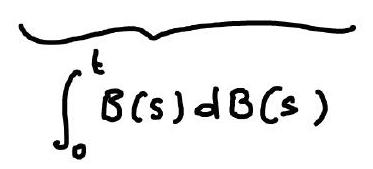
\includegraphics[width=0.5\textwidth]{graphics/2025_10_17_a59e220b8a74630d2381g-07}
\end{figure}

\subsection*{COMMENTS:}
We recognize $X_{n}$ as the Riemann sum corresponding to $x(t)$ where we take
an arbitrary intermediate point in $\left[t_{i}, t_{i+1}\right]$. In ordinary
calculus the integral does not depend on the location of the intermediate
point, however in the stochastic integral there is an unavoidable dependence on
which point we choose. This is one of the most important features of the
stochastic calculus with Brownian motion.
proof:
We introduce a more compact notation:
$B_{i}^{\lambda} \equiv B\left(\lambda t_{i+1}+(1-\lambda) t_{i}\right), B\left(t_{i}\right) \equiv B_{i}$.
Then $X_{n}=\sum_{i=0}^{n-1} B_{i}^{\lambda}\left(B_{i+1}-B_{i}\right)$.
We use now the identity (with B.m. everything is easier with squares or squared
differences):
\begin{DispWithArrows}[displaystyle, format=c]
  \begin{aligned}
    B_{i}^{\lambda}\left(B_{i+1}-B_{i}\right) & =\left(B_{i}^{\lambda}-B_{i}+B_{i}\right)\left(B_{i+1}-B_{i}^{\lambda}+B_{i}^{\lambda}-B_{i}\right) \\
    & =\left(B_{i}^{\lambda}-B_{i}\right)\left(B_{i+1}-B_{i}^{\lambda}\right)+\left(B_{i}^{\lambda}-B_{i}\right)^{2}+B_{i}\left(B_{i+1}-B_{i}^{\lambda}\right)+B_{i}\left(B_{i}^{\lambda}-B_{i}\right) \\
    & =\left(B_{i}^{\lambda}-B_{i}\right)\left(B_{i+1}-B_{i}^{\lambda}\right)+\left(B_{i}^{\lambda}-B_{i}\right)^{2}+B_{i} B_{i+1}-B_{i}^{2} \\
    & =\underbrace{\left(B_{i}^{\lambda}-B_{i}\right)\left(B_{i+1}-B_{i}^{\lambda}\right)}_{(\text{D})}+\underbrace{\left(B_{i}^{\lambda}-B_{i}\right)^{2}}_{(\text{C})}-\underbrace{\frac{1}{2}\left(B_{i+1}-B_{i}\right)^{2}}_{(\text{B})}+\underbrace{\frac{B_{i+1}^{2}}{2}-\frac{B_{i}^{2}}{2}}_{(A)}
  \end{aligned}
\end{DispWithArrows}
Let's calculate all the terms:
(A)
$\sum_{i=0}^{n-1}\left(\frac{B_{i+1}^{2}}{2}-\frac{B_{i}^{2}}{2}\right)=\frac{1}{2}\left(B_{n}^{2}-B_{0}^{2}\right)=\frac{B^{2}(t)}{2}$
(B)
$-\frac{1}{2} \sum_{i=0}^{n-1}\left(B_{i+1}-B_{i}\right)^{2} \xrightarrow{\text{ms-limit}} -\frac{t}{2}$
(lemma)
(C)
$\sum_{i=0}^{n-1}\left(B_{i}^{\lambda}-B_{i}\right)^{2} \xrightarrow{\text{ms-limit}} \lambda t$
(use the lemma)
(D) We have to show that the term (D) is zero in the ms-limit:
\begin{DispWithArrows}[displaystyle, format=c]
  \begin{aligned}
    \mathbb{E}\left[\left(\sum_{i=0}^{n-1}\left(B_{i}^{\lambda}-B_{i}\right)\left(B_{i+1}-B_{i}^{\lambda}\right)\right)^{2}\right] & =\sum_{i=0}^{n-1} \mathbb{E}\left[\left(B_{i}^{\lambda}-B_{i}\right)^{2}\right] \mathbb{E}\left[\left(B_{i+1}-B_{i}^{\lambda}\right)^{2}\right] \\
    & =\sum_{i=0}^{n-1} \lambda\left(t_{i+1}-t_{i}\right) \cdot(1-\lambda)\left(t_{i+1}-t_{i}\right) \\
    & \leq \lambda(1-\lambda) \max _{j}\left(t_{j+1}-t_{j}\right) \sum_{i=0}^{n-1}\left(t_{i+1}-t_{i}\right) \leq \lambda(1-\lambda)\left|\mathcal{P}_{n}\right| t \rightarrow 0 \text { as } n \rightarrow
    \infty .
  \end{aligned}
\end{DispWithArrows}
The theorem shows that
\begin{DispWithArrows}[displaystyle, format=c]
  \int_{0}^{t} B(s) d B(s)=\frac{B^{2}(t)}{2}+\left(\lambda-\frac{1}{2}\right) t
\end{DispWithArrows}
so it does depend in general on the intermediate point that we choose. The main
choices are:
(I) $\int_{0}^{t} B(s) d B(s)=\frac{B^{2}(t)}{2}-\frac{t}{2} \quad$ Itô integral,
$\lambda=0$
(S) $\int_{0}^{t} B(s) d B(s)=\frac{B^{2}(t)}{2} \quad$ Stratonovich integral,
$\lambda=\frac{1}{2}$

\subsection*{IMPORTANT COMMENTS:}
(1) Why should we use Itô? Since $t$ represents time and because we do not know
what value B will get in the following interval $\left[t_{i}, t_{i+1}\right]$,
we prefer to select the known value in the approximation, i.e.
$B\left(t_{i}\right)$. This is the choice in (I).

From eq. (32)
\begin{DispWithArrows}[displaystyle, format=c]
  \mathbb{E}\left[\int_{0}^{t} B(s) d B(s)\right]=0
\end{DispWithArrows}
So (I) has the strange property that that it does not follow ordinary calculus,
but it is handy because one can show that
$\mathbb{E}[B(t) d B(t)]=\mathbb{E}[B(t)] \mathbb{E}[d B(t)]=0$. In general for
Itô integrals:
\begin{DispWithArrows}[displaystyle, format=c]
  E\left[\int \sigma d B\right]=\int E[\sigma] E[d B]=0
\end{DispWithArrows}
In the following we will always use the Itô prescription when considering SDEs
of the form (28).

Notice that if the SDE is with additive noise (eq. (27)) there is no need to
introduce any intermediate prescription.
If we use a function $\sigma(x)$, instead of $B(s)$, and we define
$\int_{0}^{t} \sigma(x) d B(s)$ as in eq. (28b), in general $\sigma(x)$ will
depend on the B.m. $B(s)$ for $s \leq t$ and we do not know at time $t$ its
future value at times $\tau>t$. We don't want $\sigma$ to depend on
$B(\tau)-B(s), \forall \tau>s$. All these functions $\sigma(x)$, which depend
only on the information available up to time $t$ (so they are indep. of
$B(\tau)-B(s), \forall \tau>s$), are called non-anticipating functions. We will
always use these functions.
If $\sigma$ is non-anticipating, the Itô stochastic integral ($\lambda=0$) of
the function $\sigma(x)$ is defined as
\begin{DispWithArrows}[displaystyle, format=c]
  \int_{0}^{t} \sigma(s) d B(s)=\lim _{n \rightarrow
      \infty} \left(\sum_{i=0}^{n-1} \sigma\left(t_{i}\right)\left[B\left(t_{i+1}\right)-B\left(t_{i}\right)\right]\right)
\end{DispWithArrows}
One can also show that ($\sigma$ non-anticipating)
\begin{DispWithArrows}[displaystyle, format=c]
  \left\langle\left(\int_{0}^{t} \sigma(s) d B(s)\right)^{2}\right\rangle=\int_{0}^{t} d s \left\langle\sigma(s)^{2}\right\rangle
\end{DispWithArrows}
(See Gardiner p. 84):
$\operatorname{ms-lim} \sum_{i=0}^{n-1} \sigma_{i}^{2}\left(B_{i+1}-B_{i}\right)^{2}=\int_{0}^{t} d s \sigma(s)^2$
(2) The advantage with the Stratonovich choice ($\lambda=\frac{1}{2}$) is that
one can use ordinary calculus, but in this case
\begin{DispWithArrows}[displaystyle, format=c]
  \mathbb{E}\left[\int_{0}^{t} B(s) d B(s)\right]=\frac{t}{2}
\end{DispWithArrows}
So the B.m. is correlated to the following times.

The dependence on the intermediate point is clear even when calculating the
expected value $\mathbb{E}\left[\int_{0}^{t} B(s) d B(s)\right]$.
The discretization gives ($t_{0}=0, t_{n}=t$)
\begin{DispWithArrows}[displaystyle, format=c]
  \begin{aligned}
    & \mathbb{E}\left[\sum_{i=0}^{n-1} B\left(t_{i}+\lambda\left(t_{i+1}-t_{i}\right)\right)\left(B\left(t_{i+1}\right)-B\left(t_{i}\right)\right)\right]=
    \\
    = & \sum_{i} \mathbb{E}\left[B\left(t_{i}+\lambda\left(t_{i+1}-t_{i}\right)\right) B\left(t_{i+1}\right)\right]-\sum_{i}\mathbb{E}\left[B\left(t_{i}+\lambda\left(t_{i+1}-t_{i}\right)\right) B\left(t_{i}\right)\right] \\
    = & \sum_{i=0}^{n-1} \left(t_{i}+\lambda\left(t_{i+1}-t_{i}\right)-t_{i}\right)=\lambda t
  \end{aligned}
\end{DispWithArrows}
Exercise: Assume that the stochastic process $g(t)$ depends on the B.m. $B(s)$
for any $s<t$, so $g$ is non-anticipating. Show that
$\mathbb{E}\left[\left(\int_{0}^{t} g(s) d B(s)\right)^{2}\right]=\mathbb{E}\left[\int_{0}^{t} g^{2}(s) d s\right]$
if we use the Itô convention.
Hint: use the discretization
$\sum_{i=0}^{n-1} g\left(t_{i}\right)\left(B\left(t_{i+1}\right)-B\left(t_{i}\right)\right)$
and, after all the calculations, take the limit $n \rightarrow
\infty$.

\subsection*{Itô Calculus}
We have seen that the Brownian motion may lead to a change in the usual
calculus. In the following we only show what are the new differentiation rules
when using the Itô prescription and the finding that $\Delta B \simeq \sqrt{\Delta t}$
Let's assume that $u(B(t), t)$, then
\begin{DispWithArrows}[displaystyle, format=c]
  \begin{aligned}
    \Delta u & =u(B(t+\Delta t), t+\Delta t)-u(B(t), t) \stackrel{\downarrow}{=} \frac{\partial u}{\partial t} \Delta t+\frac{\partial u}{\partial B} \Delta B+\frac{1}{2} \frac{\partial^{2} u}{\partial B^{2}} \Delta B^{2}+\text { h.o.t. } \\
    & =\left(\frac{\partial u}{\partial t}+\frac{1}{2} \frac{\partial^{2} u}{\partial B^{2}}\right) \Delta t+\frac{\partial u}{\partial B} \Delta B \quad \leftarrow \text { " } \Delta B^{2}=\Delta t 	ext " \\
    & =\left(\frac{\partial u}{\partial t}+\frac{1}{2} \frac{\partial^{2} u}{\partial B^{2}}\right) \Delta t+\frac{\partial u}{\partial B} \Delta B
  \end{aligned}
\end{DispWithArrows}
this term is not present in ordinary calculus and is due to the fact that $| 
\Delta B| \simeq \sqrt{\Delta t}$

The Itô differential rule is
\begin{DispWithArrows}[displaystyle, format=c]
  d u=\left(\frac{\partial u}{\partial t}+\frac{1}{2} \frac{\partial^{2} u}{\partial B^{2}}\right) d t+\frac{\partial u}{\partial B} d B
\end{DispWithArrows}
Of course, if $u$ does not depend on $t$,
$d u=\frac{1}{2} \frac{\partial^{2} u}{\partial B^{2}} d t+\frac{\partial u}{\partial B} d B$.
Example: $u(B)=B^{2}$, then $d B^{2}=d t+2 B d B$. If we then integrate both
sides
$\int_{t_{1}}^{t_{2}} d\left(B^{2}\right)=B^{2}\left(t_{2}\right)-B^{2}\left(t_{1}\right)=t_{2}-t_{1}+2 \int_{t_{1}}^{t_{2}} B(s) d B(s)$
we get
\begin{DispWithArrows}[displaystyle, format=c]
  \int_{t_{1}}^{t_{2}} B(s) d B(s)=\frac{B^{2}\left(t_{2}\right)-B^{2}\left(t_{1}\right)}{2}-\frac{t_{2}-t_{1}}{2}
\end{DispWithArrows}
which is in agreement with eq. (I)

Exercise: 1) Calculate the Itô differential for $B_{t}^{n}$ and show that
$d B_{t}^{n}=n B_{t}^{n-1} d B_{t}+\frac{n(n-1)}{2} B_{t}^{n-2} d t$ and
$\int_{0}^{t} B^{n} d B=\frac{B_{t}^{n+1}}{n+1}-\frac{n}{2} \int_{0}^{t} B(s)^{n-1} d s$
2) By using the Itô differential of $Y(B, t)=e^{\lambda B(t)-\frac{\lambda^{2}}{2} t}$
and that $B(0)=0$, show that $Y(t)=Y(B, t)$ solves the Itô SDE
\begin{DispWithArrows}[displaystyle, format=ll]
  \left\{
    \begin{aligned}
      & d Y(t) \quad=\lambda Y(t) d B(t) \\
      & Y(0) \quad=1
    \end{aligned}\right.
\end{DispWithArrows}
Show that $\langle Y(t)\rangle=1 \quad \forall t \geqslant 0$ and
$P(y, t)=\frac{e^{-\frac{\left(\ln y+\frac{\lambda^{2} t}{2}\right)^{2}}{2 \lambda^{2} t}}}{\sqrt{2 \pi \lambda^{2} t}} y$.
This is called log-normal distribution.

\subsection*{Itô's chain rule (Itô's formula)}
Suppose that $X(t)$ is a stoch. process which satisfies the SDE
\begin{DispWithArrows}[displaystyle, format=c]
  d x(t)=\mu(x, t) d t+\sigma(x, t) d B(t)
\end{DispWithArrows}
where the SDE is interpreted with the Itô prescription; then if
$u(x, t) \in C_{t}^{1}, \in C_{x}^{2}$ then the stochastic process $u$ satisfies
the SDE:
\begin{DispWithArrows}[displaystyle, format=c]
  d u=\left(\frac{\partial u}{\partial t}+\frac{\partial u}{\partial x} \mu+\frac{1}{2} \frac{\partial^{2} u}{\partial x^{2}} \sigma^{2}\right) d t+\frac{\partial u}{\partial x} \sigma d B
\end{DispWithArrows}
Indeed, we use the simple rules:
$d t d B=O\left(d t^{3 / 2}\right), d B^{2}=d t$
\begin{DispWithArrows}[displaystyle, format=c]
  d u=\frac{\partial u}{\partial t} d t+\frac{\partial u}{\partial x} d x+\frac{1}{2} \frac{\partial^{2} u}{\partial x^{2}} d x^{2}+\text { h.o.t. } \\
  \text { however } d x^{2}=(\mu d t+\sigma d B)^{2}=\mu^{2} d t^{2}+2 \mu \sigma d t d B+\sigma^{2} d B^{2}=\sigma^{2} d t
\end{DispWithArrows}
then
\begin{DispWithArrows}[displaystyle, format=c]
  \begin{aligned}
    d u & =\frac{\partial u}{\partial t} d t+\frac{\partial u}{\partial x}(\mu d t+\sigma d B)+\frac{1}{2} \frac{\partial^{2} u}{\partial x^{2}} \sigma^{2} d t \\
    & =\left(\frac{\partial u}{\partial t}+\frac{\partial u}{\partial x} \mu+\frac{1}{2} \frac{\partial^{2} u}{\partial x^{2}} \sigma^{2}\right) d t+\frac{\partial u}{\partial x} \sigma d B \text { as in (35) }
  \end{aligned}
\end{DispWithArrows}
Exercise: 1) The stoch. proc. $x(t)$ satisfies the Itô SDE (This process is
called geometric Brownian motion).
\begin{DispWithArrows}[displaystyle, format=ll]
  \left\{
    \begin{aligned}
      d x&=\frac{x}{2} d t+x d B \\
      x(0)&=1
    \end{aligned}\right.
\end{DispWithArrows}
Show that the process $y=\ln x$ satisfies the Itô SDE
\begin{DispWithArrows}[displaystyle, format=ll]
  \left\{
    \begin{aligned}
      d y&=d B \\
      y(0)&=0
    \end{aligned}\right.
\end{DispWithArrows}
and therefore the solution of the original SDE is $x(t)=e^{B(t)}$.
2) Itô formula for 2 variables:

Assume that the two processes $x(t)$ and $y(t)$ satisfy the two Itô SDEs
$d x=\mu_{x} d t+\sigma_{x} d B$ and $d y=\mu_{y} d t+\sigma_{y} d B$. By using
the Itô rules, show that if $u(x, y) \in C^{2}(x, y)$ then
$d u=\left(\frac{\partial u}{\partial x} \mu_{x}+\frac{\partial u}{\partial y} \mu_{y}+\frac{1}{2} \frac{\partial^{2} u}{\partial x^{2}} \sigma_{x}^{2}+\frac{1}{2} \frac{\partial^{2} u}{\partial y^{2}} \sigma_{y}^{2}+\frac{\partial^{2} u}{\partial x \partial y} \sigma_{x} \sigma_{y}\right) d t+\left(\frac{\partial u}{\partial x} \sigma_{x}+\frac{\partial u}{\partial y} \sigma_{y}\right) d B$
Take $u(x, y)=x y$, then one can write
\begin{DispWithArrows}[displaystyle, format=c]
  d(x y)=\left(x \mu_{y}+y \mu_{x}+\sigma_{x} \sigma_{y}\right) d t+\left(x \sigma_{y}+y \sigma_{x}\right) d B
\end{DispWithArrows}
and deduce the correlation between the two processes $x$ and $y$
3) The Ornstein-Uhlenbeck process is defined by the SDE:
\begin{DispWithArrows}[displaystyle, format=ll]
  \left\{
    \begin{aligned}
      d x&=-\mu x d t+\sigma d B \\
      x(0)&=x_{0}
    \end{aligned}\right.
\end{DispWithArrows}
In order to solve the SDE, show that the SDE of $y(t)=e^{\mu t} x(t)$ is
$d y=\sigma e^{\mu t} d B$, hence
$y(t)=y(0)+\sigma \int_{0}^{t} e^{\mu s} d B(s)$ and finally
\begin{DispWithArrows}[displaystyle, format=c]
  x(t)=e^{-\mu t}\left(x_{0}+\sigma \int_{0}^{t} e^{\mu s} d B(s)\right)
\end{DispWithArrows}
Ex: Find the solution of the SDE $d x=( \eta-\mu x) d t+\sigma d B$.
Of course, $\mathbb{E}(x(t))=x_{0} e^{-\mu t}$. We calculate now
$\left\langle x^{2}(t)\right\rangle$.
\begin{DispWithArrows}[displaystyle, format=ll]
  \begin{aligned}
    d\left(x^{2}\right) & =2 x d x+d x^{2}=2 x(-\mu x d t+\sigma d B)+(-\mu x d t+\sigma d B)^{2} \\
    & =\left(-2 \mu x^{2}+\sigma^{2}\right) d t+2 \sigma x d B \\
    \frac{d}{d t}\left\langle x^{2}\right\rangle & =-2 \mu\left\langle x^{2}\right\rangle+\sigma^{2}+2 \sigma\left\langle x \frac{d B}{d t}\right\rangle=-2 \mu\left\langle x^{2}\right\rangle+\sigma^{2} \\
    \left\langle x(t)^{2}\right\rangle & =\frac{\sigma^{2}}{2 \mu}+\left(x_{0}^{2}-\frac{\sigma^{2}}{2 \mu}\right) e^{-2 \mu t}
  \end{aligned}
\end{DispWithArrows}
Thus
$\operatorname{Var}[x(t)]=\left\langle x(t)^{2}\right\rangle-\langle x(t)\rangle^{2}=\frac{\sigma^{2}}{2 \mu}\left(1-e^{-2 \mu t}\right)$

For a stoch. proc. like $x(t)$ we can calculate the auto-correlation
$c(t, s)=\langle x(t) x(s)\rangle-\langle x(t)\rangle\langle x(s)\rangle$.
As you see from eq. (36), we have to calculate averages of this kind
\begin{DispWithArrows}[displaystyle, format=c]
  \mathbb{E}\left[\int_{0}^{t} G\left(t^{\prime}\right) d B\left(t^{\prime}\right) \int_{0}^{s} H
    \left(s^{\prime}\right) d B\left(s^{\prime}\right)\right]
\end{DispWithArrows}
Where $G$ and $H$ are both cont. and non-anticipating. As usual we have to
discretize: take $t>s,(n>m)$
\begin{DispWithArrows}[displaystyle, format=c]
  \begin{aligned}
    & \mathbb{E}\left[\sum_{i=0}^{n-1} G_{i}\left(B_{i+1}-B_{i}\right) \sum_{j=0}^{m-1} H_{j}\left(B_{j+1}-B_{j}\right)\right]=
    \\
    = & \mathbb{E}\left[\sum_{i=0}^{m-1} G_{i}\left(B_{i+1}-B_{i}\right) \sum_{j=0}^{m-1} H_{j}\left(B_{j+1}-B_{j}\right)\right]+\mathbb{E}\left[\sum_{i=m}^{n-1} \ldots \sum_{j=0}^{m-1} \ldots\right] \\
    = & \mathbb{E}\left[\sum_{i=0}^{m-1} G_{i} H_{i}\left(B_{i+1}-B_{i}\right)^{2}\right]+2 \mathbb{E}\left[\sum_{i \neq j}^{m-1} G_{i}\left[B_{i+1}-B_{i}\right] H_{j}
      \left[B_{j+1}-B_{j}\right]\right]=
    \\
    = & \mathbb{E}\left[\sum_{i=0}^{m-1} G_{i} H_{i}\left(B_{i+1}-B_{i}\right)^{2}\right]
  \end{aligned}
\end{DispWithArrows}
now by taking the limit $m \rightarrow
\infty$
\begin{DispWithArrows}[displaystyle, format=c]
  \longrightarrow \mathbb{E}\left[\int_{0}^{s} G\left(s^{\prime}\right) H\left(s^{\prime}\right) d s^{\prime}\right]=\int_{0}^{s} \mathbb{E}\left[G\left(s^{\prime}\right) H\left(s^{\prime}\right)\right] d s^{\prime}
\end{DispWithArrows}
If we re-do the calculations for $t<s$, we can convince ourselves that
\begin{DispWithArrows}[displaystyle, format=c]
  \mathbb{E}\left[\int_{0}^{t} G\left(t^{\prime}\right) d B\left(t^{\prime}\right) \int_{0}^{s} H
    \left(s^{\prime}\right) d B\left(s^{\prime}\right)\right]=\int_{0}^{t \wedge s} \mathbb{E}\left[G\left(s^{\prime}\right) H\left(s^{\prime}\right)\right] d s^{\prime}
\end{DispWithArrows}
Now let's use eq. (39) to calculate the auto-correlation function of the O-U
process, whose solution is in eq. (36)
\begin{DispWithArrows}[displaystyle, format=c]
  \begin{aligned}
    \mathbb{E}[x(t) x(s)] & =\mathbb{E}\left[e^{-\mu t}\left(x_{0}+\sigma \int_{0}^{t} e^{\mu t^{\prime}} d B\left(t^{\prime}\right)\right) e^{-\mu s}\left(x_{0}+\sigma \int_{0}^{s} e^{\mu s^{\prime}} d B\left(s^{\prime}\right)\right)\right] \\
    & =x_{0}^{2} e^{-\mu(t+s)}+\sigma^{2} e^{-\mu(t+s)} \int_{0}^{t
        \wedge s} e^{2
        \mu s^{\prime}} d s^{\prime} \\
    & =x_{0}^{2} e^{-\mu(t+s)}+\frac{\sigma^{2}}{2
        \mu} e^{-\mu(t+s)}\left(e^{2
        \mu(t
        \wedge s)}-1\right) \\
    & =x_{0}^{2} e^{-\mu(t+s)}+\frac{\sigma^{2}}{2
        \mu}\left(e^{-\mu|t-s|}-e^{-\mu(t+s)}\right)
  \end{aligned}
\end{DispWithArrows}
And therefore the (connected) auto-correlation function is
\begin{DispWithArrows}[displaystyle, format=c]
  c(t, s)=\frac{\sigma^{2}}{2
      \mu}\left(e^{-\mu|t-s|}-e^{-\mu(t+s)}\right)
\end{DispWithArrows}
If we start from some distribution $p
\left(x_{0}\right)$ for the initial conditions, we get
\begin{DispWithArrows}[displaystyle, format=c]
  c(t, s)=\operatorname{Var}\left(x_{0}\right) e^{-\mu(t+s)}+\frac{\sigma^{2}}{2
      \mu}\left(e^{-\mu|t-s|}-e^{-\mu(t+s)}\right)
\end{DispWithArrows}
Notice that, if we let $t, s \rightarrow
\infty$ but $t-s$ is fixed, then from (40) we get
\begin{DispWithArrows}[displaystyle, format=c]
  C_{ \text {stat }}(|t-s|)=\frac{\sigma^{2}}{2
      \mu} e^{-\mu|t-s|}
\end{DispWithArrows}
which only depends on $|t-s|$. This is the stationary autocorrelation function
of the O.-U. process which does not depend on any initial condition!
% !TeX encoding = UTF-8
% Lecture file created by newnote
% Class: Models of Theoretical Physics
% Professor: Azaele Sandro
% Date: 2025-10-03
\lecture{11}{Gaussian Integrals continued}{2025-10-03}
\pagelayout{margin}
% --- Start writing here ---

\section{Gaussian Integrals continued}
\begin{DispWithArrows}[displaystyle, format=c]
  \int_{-\infty}^{+\infty} e^{-\frac{a x^{2}}{2}+b x} d x=\sqrt{\frac{2 \pi}{a}} e^{\frac{b^{2}}{2 a}} \quad a>0, b \in \mathbb{C}
\end{DispWithArrows}
\begin{DispWithArrows}[displaystyle, format=c]
  \varphi(k)=\int e^{i k x} p(x) d x=\left\langle e^{i k x}\right\rangle
\end{DispWithArrows}
\begin{DispWithArrows}[displaystyle, format=c]
  \left.(-i)^{n} \frac{d^{n} \varphi}{d k^{n}}\right|_{k=0}=\left\langle x^{n}\right\rangle
\end{DispWithArrows}
\begin{DispWithArrows}[displaystyle, format=c]
  \int_{-\infty}^{+\infty} \frac{1}{\sqrt{2 \pi \sigma^{2}}} e^{-\frac{x^{2}}{2 \sigma^{2}}} e^{i k x} d x=e^{-\frac{\sigma^{2} k^{2}}{2}}
\end{DispWithArrows}
Because of eq. (5)
\begin{DispWithArrows}[displaystyle, format=c]
  \langle x\rangle=-\left.i \frac{d}{d k} e^{-\frac{\sigma^{2} k^{2}}{2}}\right|_{k=0}=0
\end{DispWithArrows}
Important Gaussian integrals:
$\left\langle x^{n}\right\rangle=\left.(-i)^{n} \frac{d^{n}}{d k^{n}} e^{-\frac{\sigma^{2} k^{2}}{2}}\right|_{k=0}=0$
if $n$ is odd (by symmetry).
However
\begin{DispWithArrows}[displaystyle, format=c]
  \left\langle x^{4}\right\rangle=\left.\frac{d^{4}}{d k^{4}} e^{-\frac{\sigma^{2} k^{2}}{2}}\right|_{k=0}=\left[\sigma^{4}\left(3-6 k^{2} \sigma^{2}+k^{4} \sigma^{4}\right) e^{-\frac{\sigma^{2} k^{2}}{2}}\right]_{k=0} = 3 \sigma^{4}=\frac{1}{\sqrt{2 \pi \sigma^{2}}} \int_{-\infty}^{+\infty} e^{-\frac{x^{2}}{2 \sigma^{2}}} x^{4} d x .
\end{DispWithArrows}
If we want to calculate $\left\langle x^{n}\right\rangle$, we better start from
\begin{DispWithArrows}[displaystyle, format=c]
  \int_{-\infty}^{+\infty} e^{-\frac{a x^{2}}{2}} d x=\sqrt{\frac{2 \pi}{a}}
\end{DispWithArrows}
We differentiate both sides wrt a:
once
\begin{DispWithArrows}[displaystyle, format=c]
  \int_{-\infty}^{+\infty} x^{2} e^{-\frac{a x^{2}}{2}} d x=\frac{\sqrt{2 \pi}}{a^{3 / 2}} \rightarrow\left\langle x^{2}\right\rangle
\end{DispWithArrows}
twice
\begin{DispWithArrows}[displaystyle, format=c]
  \int_{-\infty}^{+\infty} x^{4} e^{-\frac{a x^{2}}{2}} d x=\frac{3 \sqrt{2 \pi}}{a^{5 / 2}}
\end{DispWithArrows}
$n/2$ times, $n$ is even
\begin{DispWithArrows}[displaystyle, format=c]
  \int_{-\infty}^{+\infty} x^{n} e^{-\frac{a x^{2}}{2}} d x=\frac{(n-1)!! \sqrt{2 \pi}}{a^{(n+1) / 2}}
\end{DispWithArrows}
From this find the expression of $\left\langle x^{n}\right\rangle$ as a
function of $\sigma$ and $n$ (even).

\subsection*{Multidimensional Gaussian Integrals}
Example:
\begin{DispWithArrows}[displaystyle, format=c]
  \int_{-\infty}^{+\infty} d x_{1} \int_{-\infty}^{+\infty} d x_{2} e^{-\frac{3}{2}\left(x_{1}^{2}+x_{2}^{2}\right)+x_{1} x_{2}}=?
\end{DispWithArrows}
Ex: write down the exponent in the form
$-\frac{1}{2} \vec{x}^{\top} A \vec{x}$.
More generally,
\begin{DispWithArrows}[displaystyle, format=c]
  Z(A)=\int_{\mathbb{R}^{m}} d^{m}x e^{-\frac{1}{2} \vec{x}^{\top} A \vec{x}}
\end{DispWithArrows}
Where $\vec{x}=\left(x_{1}, \ldots, x_{m}\right)$ and the matrix $A$ is
diagonalizable with strictly positive eigenvalues (positive definite). Then
there exist an orthogonal matrix
$O \quad\left(\Rightarrow O O^{\top}=O^{\top} O=\mathbb{1}\right)$ such that we
can define $\vec{y}=O \vec{x}$ and $O A O^{\top}=\Lambda$
\begin{DispWithArrows}[displaystyle, format=c]
  \Lambda=\begin{pmatrix}
    \lambda_{1} & & 0 \\ \nonumber
    & \ddots & \\ \nonumber
    0 & & \lambda_{m}
  \end{pmatrix} \quad \lambda_{i}>0 \quad i=1,2, \ldots m
\end{DispWithArrows}
It follows that
\begin{DispWithArrows}[displaystyle, format=c]
  \vec{x}^{\top} A \vec{x}=\vec{x}^{\top} O^{\top} \Lambda O \vec{x}=\vec{y}^{\top} \Lambda \vec{y}
\end{DispWithArrows}
$Z(A)=\int d^{m}x e^{-\frac{1}{2} \vec{x}^{\top} A \vec{x}}=\int d^{m}y\left|\frac{\partial \vec{x}}{\partial \vec{y}}\right| e^{-\frac{1}{2} \vec{y}^{\top} \Lambda \vec{y}}$
determinant of the Jacobian:
$\left|\frac{\partial \vec{x}}{\partial \vec{y}}\right|=\operatorname{det}\left(O^{\top}\right)=1$
(show as an exercise.)
\begin{DispWithArrows}[displaystyle, format=c]
  \vec{y}^{\top} \Lambda \vec{y}=\sum_{i j} y_{i} \Lambda_{i j} y_{j}=\sum_{i j} y_{i} \lambda_{i} \delta_{i j} y_{j}=\sum_{i} \lambda_{i} y_{i}^{2}
\end{DispWithArrows}
From this we get
\begin{DispWithArrows}[displaystyle, format=c]
  \begin{aligned}
    & =\int_{\mathbb{R}^{m}} d^{m} y e^{-\frac{1}{2} \sum_{i} \lambda_{i} y_{i}^{2}}=\prod_{i=1}^{m} \int_{-\infty}^{+\infty} d y_{i} e^{-\frac{1}{2} \lambda_{i} y_{i}^{2}}=\prod_{i=1}^{m} \sqrt{\frac{2 \pi}{\lambda_{i}}}=\frac{(2 \pi)^{m / 2}}{\sqrt{\lambda_{1} \cdots \lambda_{m}}} \\ \nonumber
    & \operatorname{det}(A)=\operatorname{det}\left(O^{\top} \Lambda O\right)=\operatorname{det}(\Lambda)(\operatorname{det} O)^{2}=\operatorname{det} \Lambda=\lambda_{1} \cdots \lambda_{m}
  \end{aligned}
\end{DispWithArrows}
Hence
\begin{DispWithArrows}[displaystyle, format=c]
  Z(A)=\frac{(2 \pi)^{m / 2}}{\sqrt{\operatorname{det} A}}=\int_{\mathbb{R}^{m}} d^{m}x e^{-\frac{1}{2} \vec{x}^{\top} A \vec{x}}
\end{DispWithArrows}
By using (8) show that
\begin{DispWithArrows}[displaystyle, format=c]
  \int_{-\infty}^{+\infty} d x_{1} \int_{-\infty}^{+\infty} d x_{2} e^{-\frac{3}{2}\left(x_{1}^{2}+x_{2}^{2}\right)+x_{1} x_{2}}=\frac{\pi}{\sqrt{2}}
\end{DispWithArrows}
Exercise: Let
$p(x, y)=\frac{\sqrt{\operatorname{det} A}}{2 \pi} e^{-\frac{1}{2}\left(a_{11} x^{2}+2 a_{12} x y+a_{22} y^{2}\right)}$
where $a_{11}, a_{22}>0$. Show that $q(x)=\int p(x, y) dy$ is still a Gaussian
distribution. Find the corresponding variance of $x$. This is also true for
m-dimension Gaussian variables.

We want now to calculate
\begin{DispWithArrows}[displaystyle, format=c]
  Z(A, \vec{b})=\int d^{m} x e^{-\frac{1}{2} \vec{x}^{\top} A \vec{x}+\vec{x}^{\top} \cdot \vec{b}}
\end{DispWithArrows}
we use the same strategy we used before:
\begin{DispWithArrows}[displaystyle, format=c]
  \vec{\nabla}_{x}\left(-\frac{1}{2} \vec{x}^{\top} A \vec{x}+\vec{x}^{\top} \cdot \vec{b}\right)=-A \vec{x}+\vec{b}=0 \Rightarrow \vec{x}=A^{-1} \vec{b} \quad (\text{if }\det A \neq 0)
\end{DispWithArrows}
We introduce
\begin{DispWithArrows}[displaystyle, format=ll]
  \begin{aligned}
    \vec{y} & =\vec{x}-A^{-1} \vec{b} \\ \nonumber
    -\frac{1}{2} \vec{x}^{\top} A \vec{x}+\vec{x}^{\top} \cdot \vec{b} & =-\frac{1}{2} \vec{y}^{\top} A \vec{y}+\frac{\vec{b}^{\top} A^{-1} \vec{b}}{2} \quad \text { (do the calculation). }
  \end{aligned}
\end{DispWithArrows}
Hence
\begin{DispWithArrows}[displaystyle, format=c]
  Z(A, \vec{b})=\int_{\mathbb{R}^{m}} d^{m}y e^{-\frac{1}{2} \vec{y}^{\top} A \vec{y}+\frac{\vec{b}^{\top} A^{-1} \vec{b}}{2}}=e^{\frac{\vec{b}^{\top} A^{-1} \vec{b}}{2}} Z(A, 0)
\end{DispWithArrows}
\begin{DispWithArrows}[displaystyle, format=c]
  Z(A, \vec{b})=\frac{(2 \pi)^{m / 2}}{\sqrt{\operatorname{det} A}} e^{\frac{\vec{b}^{\top} A^{-1} \vec{b}}{2}}
\end{DispWithArrows}
Eq. (10) allows to find the charact. function of the multivariate Gaussian
distrib.
\begin{DispWithArrows}[displaystyle, format=c]
  p(\vec{x})=\frac{1}{Z(A, 0)} e^{-\frac{1}{2} \vec{x}^{\top} A \vec{x}}
\end{DispWithArrows}
\begin{DispWithArrows}[displaystyle, format=c]
  \int_{\mathbb{R}^{m}} d^{m}x p(x) e^{i \vec{k} \cdot \vec{x}}=e^{-\frac{\vec{k}^{\top} A^{-1} \vec{k}}{2}}=\varphi(k)
\end{DispWithArrows}
What is the meaning of $A^{-1}$?
The definition of the ch. f. in the multidim. case is:
\begin{DispWithArrows}[displaystyle, format=c]
  \varphi(\vec{k})=\int d^{m}x e^{i \vec{k} \cdot \vec{x}} p(\vec{x}) \quad \vec{k}=\left(k_{1}, k_{2}, \ldots, k_{m}\right)
\end{DispWithArrows}
therefore we derive
\begin{DispWithArrows}[displaystyle, format=c]
  \left.(-i)^{s} \frac{\partial^s}{\partial k_{i} \partial k_{j} \cdots \partial k_{l}} \varphi(\vec{k})\right|_{\vec{k}=0}=\int d^{m} x x_{i} x_{j} \cdots x_{l} p(\vec{x})=\left\langle x_{i} x_{j} \cdots x_{l}\right\rangle
\end{DispWithArrows}
Let's calculate the 2-point correlation function for a Gaussian distr.
\begin{DispWithArrows}[displaystyle, format=c]
  \left\langle x_{i} x_{j}\right\rangle=\left.(-i)^{2} \frac{\partial}{\partial k_{i}} \frac{\partial}{\partial k_{j}} e^{-\frac{\vec{k}^{\top} A^{-1} \vec{k}}{2}}\right|_{\vec{k}=0}=\left(A^{-1}\right)_{i j}
\end{DispWithArrows}
$A^{-1}$ is the 2-point correlation function between a pair of Gauss. r.v. When
$A^{-1}$ is a diagonal matrix, we say that the vars are uncorrelated.

In the previous example:
$A=\begin{pmatrix}3 & -1 \\ -1 & 3\end{pmatrix} \quad A^{-1}=\frac{1}{8}\begin{pmatrix}3 & 1 \\ 1 & 3\end{pmatrix}$
hence
\begin{DispWithArrows}[displaystyle, format=c]
  \left\langle x_{1}^{2}\right\rangle=\frac{3}{8}=\left\langle x_{2}^{2}\right\rangle \quad\left\langle x_{1} x_{2}\right\rangle=\frac{1}{8}=\left\langle x_{2} x_{1}\right\rangle
\end{DispWithArrows}
Notice that, because of symmetry, the s-point correl. funct. for s-variable
($s$ is odd) is zero (the Gaussian remains unchanged when
$\vec{x} \rightarrow-\vec{x}$).

What happens when we calculate
$\left\langle x_{i} x_{j} \ldots x_{l}\right\rangle$?
Should we do all the derivatives like in eq. (12)? No!
If the vars are Gaussian then we can use:

\subsection*{Wick's Theorem}
Any correlation between an even number of zero-mean Gaussian r.v. can be
written down as a sum of products of 2-point correlation functions
$\left(A^{-1}\right)$.
For instance:
$\left\langle x_{a} x_{b} x_{c} x_{d}\right\rangle=\left\langle x_{a} x_{b}\right\rangle\left\langle x_{c} x_{d}\right\rangle+\left\langle x_{a} x_{c}\right\rangle\left\langle x_{b} x_{d}\right\rangle+\left\langle x_{a} x_{d}\right\rangle\left\langle x_{b} x_{c}\right\rangle$
In general
\begin{DispWithArrows}[displaystyle, format=c]
  \langle\underbrace{x_{i} x_{j} \cdots x_{m} x_{n}}_{s \text { vars }}\rangle=\sum_{p}\left(A^{-1}\right)_{i_{p} j_{p}} \cdots\left(A^{-1}\right)_{m_{p} n_{p}}
\end{DispWithArrows}
where the sum is over all possible pairings of $s$ indexes, i.e. over all ways
of grouping $s$ (even) indexes $i, j \ldots, m, n$ into pairs (counting pairs
even when indexes are equal).
Exercise: show that
\begin{DispWithArrows}[displaystyle, format=ll]
  \begin{aligned}
    & \left\langle x_{1}^{2} x_{2}^{2}\right\rangle=\left\langle x_1 x_1\right\rangle \left\langle x_2 x_2\right\rangle + 2\left\langle x_1 x_2\right\rangle^2=\frac{3}{8} \cdot \frac{3}{8}+2\left(\frac{1}{8}\right)^2=\frac{11}{64} \\ \nonumber
    & \left\langle x_{1}^{4}\right\rangle=3\left\langle x_1^2\right\rangle^2=3\left(\frac{3}{8}\right)^{2}=\frac{27}{64}
  \end{aligned}
\end{DispWithArrows}
J. Zinn-Justin, Quantum Field Theory and Critical Phenomena (ch. 1).

\subsection*{Important results obtained with characteristic functions}
If we are given the joint probability density function $p(x_{1}, x_{2})$ and it
happens that $p(x_{1}, x_{2})=p_{1}(x_{1}) p_{2}(x_{2})$ then the two vars are
independent. If, on top of this, $p_{1}=p_{2}$, then we say that the two r.v.
are independent and identically distributed (i.i.d.).

If we are given two r.v. that are i.i.d. can we calculate the distribution of
their sum?
If $x_{1} \sim q(x)$ and $x_{2} \sim q(x)$ what is the distribution of
$x=x_{1}+x_{2}$?

\section{Laplace method}
Models 14-10-25

$$ 
I(\lambda) \simeq g\left(x_{0}\right) e^{\lambda f\left(x_{0}\right)} \sqrt{\frac{2 \pi}{\lambda\left(f^{\prime \prime}\left(x_{0}\right)\right)}} 
$$ 

interion max $I(\lambda) \sim \lambda^{-1 / 2} e^{\lambda f\left(x_{0}\right)}$ endpoint (not flot) $\quad I(\lambda) \sim \lambda^{-1} e^{\lambda f\left(x_{0}\right)}$

Lp- norm in real and psis
The quontity

$$ 
\|g\|_{p}:=\left(\int_{a}^{b}|g(t)|^{p} d t\right)^{1 / p} \quad p>0 
$$ 

is colled $p$-norm when the inicynal exists (in Lestegue shase) We want to study the behavior of \|g\|p as $p \rightarrow \infty$. We assume that $g$ has a mique matimum in $t_{0}$ which is an interior point, and $g \in C^{4}(a, b)$.\We first study

$$ 
I(p) \equiv \int_{a}^{b}|g(t)|^{p} d t \quad \|g\|_{p}=I^{1 / p} 
$$ 

and

$$ 
I=\int_{a}^{b} e^{p \ln |g(t)|} d t 
$$ 

When we applied the Laplace methad we have always assumed that $f$ is continuously chifferentiable. However, if $g$ varishes somewhere in $[a, b]$ then $h / g / \rightarrow-\infty$. However, every neighborherd of points where $g=0$ will gield a negligible contribution to the initgral (i.e. to I for $p \gg 1$ ).

Thus such discontinuities con be neglected. Now we use op. (22)

$$ 
\begin{aligned}
I(p) & =e^{p \ln \left|g\left(t_{0}\right)\right|} \sqrt{\frac{2 \pi g\left(t_{0}\right)}{p\left|g^{\prime \prime}\left(t_{0}\right)\right|}}\left(1+\partial\left(\frac{1}{p}\right)\right) \\
& =\left|g\left(t_{0}\right)\right|^{p} \sqrt{\frac{2 \pi g\left(t_{0}\right)}{p\left|g^{\prime \prime}\left(t_{0}\right)\right|}}\left(1+\partial\left(\frac{1}{p}\right)\right) \text { as } p \rightarrow \infty 
\end{aligned}
$$ 

Obs: $\quad a>0 \quad a^{1 / p} p^{-\frac{1}{2 p}}=e^{\frac{\ln a}{p}} e^{-\frac{\ln p}{2 p}}$
$I^{1 / p}=\left|g\left(t_{0}\right)\right|\left(\frac{2 \pi|g|}{p\left|g^{\prime \prime}\right|}\right)^{\frac{1}{2 p}}+\operatorname{lot}=\left|g\left(t_{0}\right)\right|\left(1-\frac{\ln p}{2 p}+\sigma\left(\frac{1}{p}\right)\right)$
hence

$$ 
\|g\|_{p}=\max _{t \in[a, b]}|g(t)|\left\{1-\frac{\ln p}{2 p}+\cdots\right\} \text { as } p \rightarrow \infty 
$$ 

which gustifies the usual definition

$$ 
\|g\|\infty=\max _{t \in[a, b]}(g) 
$$ 

Example:\ Consider the integral

$$ 
\int_{0}^{\frac{3 \pi}{2}} e^{-\lambda \sin t} f(t) d t \quad \text { as } \quad \lambda \rightarrow \infty 
$$ 

where $f$ is cont. and diff. in $\left[0, \frac{3 \pi}{2}\right]$.
\begin{center}
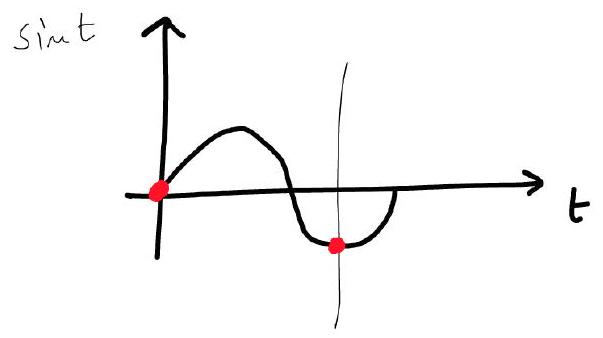
\includegraphics[width=0.5\textwidth]{2025_10_19_11b40f5928aca93f9d20g-3}
\end{center}

We want to consider the contributions from the endpoint mimima $t=0, t=\frac{3 \pi}{2}$. For this we write

$$ 
I(\lambda)=\underbrace{\int_{0}^{\pi / 2} e^{-\lambda \sin t} f(t) d t}_{I_{1}}+\underbrace{\int_{\pi / 2}^{\lambda \pi / 2} e^{-\lambda \sin t-\lambda} f(t) d t}_{I_{2}} 
$$ 

9.(24) left end point

$$ 
I_{1}=f(0) \frac{e^{\lambda \cdot 0}}{\lambda \cos (0)}=\frac{f(0)}{\lambda} \text { es } \lambda \rightarrow \infty 
$$ 

el. (23) flat enopoint

$$ 
I_{2}=f\left(\frac{3 \pi}{2}\right) e^{\lambda \cdot 0} \sqrt{\frac{\pi}{2 \lambda \sin \left(\frac{3 \pi}{2}\right)}} \simeq f\left(\frac{3 \pi}{2}\right) \sqrt{\frac{\pi}{2 \lambda}} 
$$ 

Hence the leading contribution comes from $I_{2}$ and

$$ 
I(\lambda)=f\left(\frac{3 \pi}{2}\right) e^{\lambda} \sqrt{\frac{\pi}{2 \lambda}} +\text { h.o.t. } \quad \text { as } \quad \lambda \rightarrow 0 
$$ 

The min a $t=0$ is subleadhing and it should be taken into account only at higher order.

Ex: Calculate the leading contribution to

$$ 
\int_{0}^{\pi} e^{-\lambda \sin t} f(t) d t \quad \text { as } \lambda \rightarrow \infty 
$$ 

\section*{Review of Dynomical Systems}
In mony applications (physics, biology, chemistry...) one has to study nonlinear systems of (antonomons) ODEs:

\[ 
\left\{\begin{array}{l}
\dot{\vec{x}}(t)=\vec{f}(\vec{x}(t)) \quad \tag{1} \\
\vec{x}(0)=\vec{x}_{0}
\end{array}\right. 
\] 

where $\vec{x}(t)=\left(x_{1}(t), \ldots, x_{N}(t)\right) \in U \subseteq \mathbb{R}^{N}, U$ is some open commected set of reals.
With any $\vec{x}$ we associate a vector $\vec{f}$, the set of these vectors is called vector field. The domain $U$, where $\vec{f}$ is supposed to be continuous and differentiable, is colled the phose space.
The solutions $\vec{x}\left(t, x_{0}\right)$ of the system (1) describe smooth aurves a $t$ chonges: they are called trajectories which are porometric curves in the phose space.

\section*{Example:}
Let's consider $(N=1)$

$$ 
\dot{x}(t)=\sin [x(t)] 
$$ 

$\partial_{n}$ this case the vector field is 1-chim. and coincides with the $x$-axis.
\begin{center}
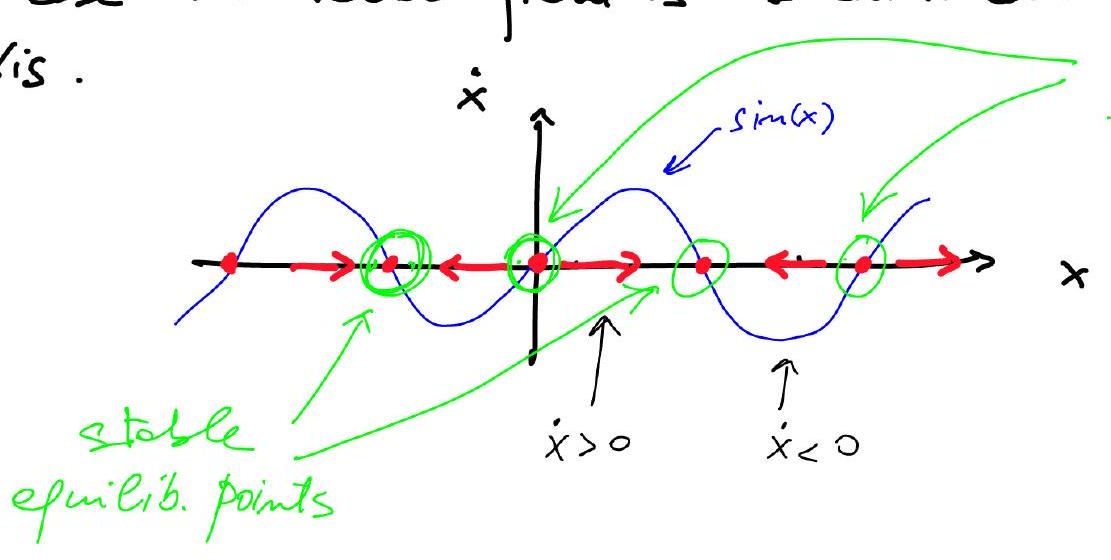
\includegraphics[width=0.5\textwidth]{2025_10_19_11b40f5928aca93f9d20g-4}
\end{center}
equil. points

In the $N=2$ cose

$$ 
\left\{\begin{array}{l}
\dot{x}=1 \ 
\dot{y}=x^{2}+y^{2}
\end{array}\right. 
$$ 

the vector field is 2 dim. and we have a map

$$ 
\vec{x}=(x, y) \longrightarrow \vec{f}(\vec{x})=\left(1, x^{2}+y^{2}\right) 
$$ 

\begin{center}
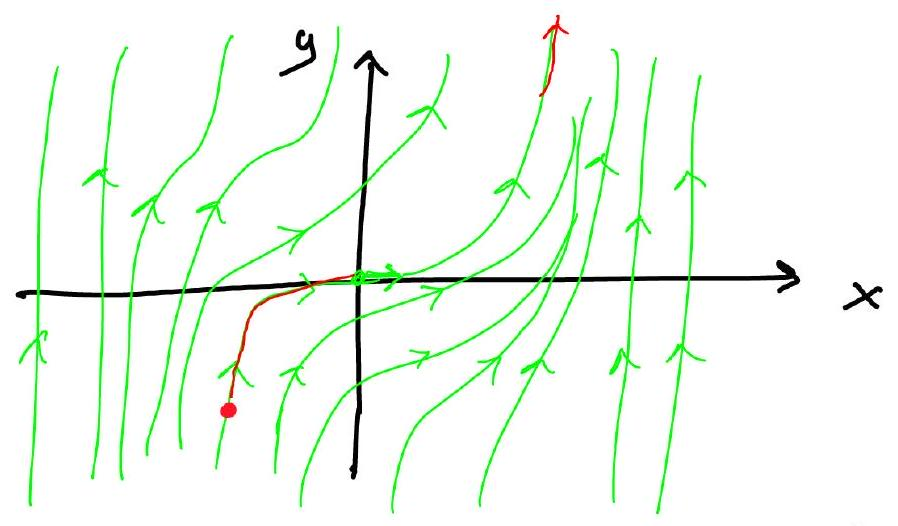
\includegraphics[width=0.5\textwidth]{2025_10_19_11b40f5928aca93f9d20g-5}
\end{center}

$$ 
\begin{array}{ll}
\hat{x} & \hat{y} \\
\dot{y}
\end{array}
$$ 

$$ 
(0,0) \longrightarrow(1,0) 
$$ 

In general the vector field $\vec{f}$ is tengent to a trajectory in every point. In fact, let $\vec{x}(t)$ be a trajectory, then the ep. of a tengent line to the trajectory at a point $\vec{x}_{a} \equiv \vec{x}\left(t_{a}\right)$ is

$$ 
\vec{Y}(u)=\vec{x}_{a}+\left(u-t_{a}\right) \dot{\vec{x}}\left(t_{a}\right)=\vec{x}_{a}+\left(u-t_{a}\right) \vec{f}\left(\vec{x}_{a}\right) 
$$ 

thus $\vec{f}$ is the directional vector of the straight line $\vec{Y}(a)$.
\begin{center}
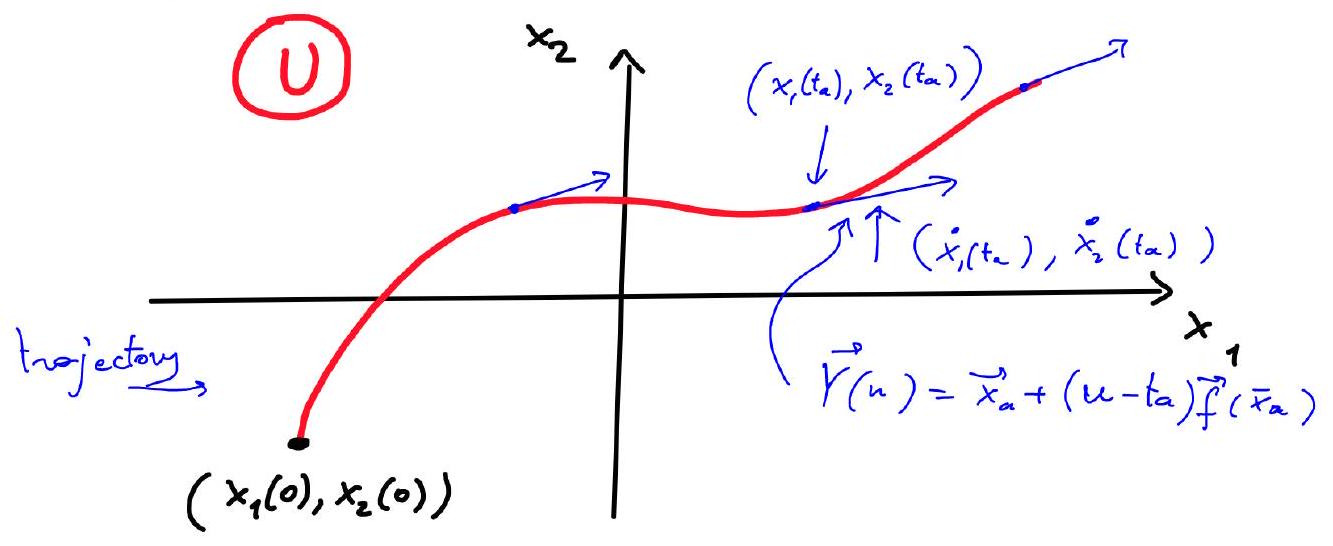
\includegraphics[width=0.5\textwidth]{2025_10_19_11b40f5928aca93f9d20g-5(1)}
\end{center}


\begin{gather*}
N=2 \ \left\{\begin{array}{l}
\dot{x}_{1}=f_{2}\\ \dot{x}_{2}=f_{2}
\end{array}\right. 	\tag{2}
\end{gather*}

By flowing along the vector field, a point traces out the trajectory $\vec{x}(t)$, a curve in the phase space $U$ or a sol. of (2).

A phose partzait is a set of trajectories with the indication of the directions of the vector field.
As we commot sobre the system (1) in general, we would like to know at least some properties.
Sometimes it is useful to study nullclines, defined es subspeces (or monifolds) where $\dot{x}_{i}=0$ for a give i. $\mathcal{H} N=2$ we may get simple curves

$$ 
\begin{array}{r}
\dot{x}_{1}=0 \Rightarrow f_{1}\\ \text { persibly } \\ x_{2}^{(1)}=g^{(1)}\\ x_{2}^{(2)}=g^{(2)}
\end{array}
$$ 

Twe interesting examples

\begin{enumerate}
  \item Find a solution of $\dot{y}=y^{2}$ with i.c. $y(0)=1$.
\end{enumerate}

Con we then find $y(2)$ ?
From $\int \frac{d y}{y^{2}}=t-c, y=\frac{1}{c-t}, y(0)=1 \Rightarrow c=1$

$$ 
y(t)=\frac{1}{1-t} \quad \rightarrow y(2)=-1 
$$ 

As $\dot{y}(t) \geqslant 0, y$ is an increasing function of time but $y(2)=-1$ ! Actually, the solution exists only in the interval $(0,1)$ as it blows up a $t=1$.
Solutions may exist only within finite intervals of time or the may not exist for some initial conditions or may not exist at all.
2) Find a solution of $j=\sqrt{y}$ for which $y(0)=0$. Find $y(2)$. 

$$ 
\int \frac{d y}{\sqrt{y}}=2 \sqrt{y}=t-c, \quad y=\frac{(t-c)^{2}}{4} \text { but } y(0)=0, y(t)=\frac{t^{2}}{4} 
$$ 

hence $y(2)=1$. But!

However $y(t)=0$ satisfies the of, and the imit. cond. Even wase:

$$ 
y(t)=\left\{\begin{array}{cc}
0 \quad 0 \leq t \leq T & T \text { is anbitary } \\
\frac{(t-T)^{2}}{4} \quad t>T & T>0 .
\end{array}\right. 
$$ 

is a solution with the same imitial constition! So there are infinitely mony solutions, so asking $y(2)$ is meomingles.
Sol. to init. val problems may not be unique.

\section*{Picard's theorem}
If $\vec{f}$ is continuous and $\frac{\partial f_{i}}{\partial x_{j}}$ are also continuous for all indexes $i j j$ in $U$, then for any $\vec{x}_{0} \in U$ the initial value problem difined in (1) admits a solution on some interval $t \in[-\delta, \delta], \delta>0$, and this salution is unique.

Obs: in this cese trajectories do not intersect.

\section*{Fixed points}
The fixed points of $\varphi$. (4) are the simplest to study as time is not relevant. Indeed, fixed points are the zeros of $\vec{f}$ : namely, $\vec{x}^{*}$ is a fixed point if


\begin{equation*}
\vec{f}\left(\vec{x}^{*}\right)=\overrightarrow{0} \quad \tag{3}
\end{equation*}


Worning: even thoyh an $O D E$ has some fixed points, that does not imply that the dymamics (the imit. Val. solut.) seach them!
% !TeX encoding = UTF-8
% Lecture file created by newnote
% Class: Models of Theoretical Physics
% Professor: Azaele Sandro
% Date: 2025-10-07
\lecture{13}{Law of large numbers}{2025-10-07}
\pagelayout{margin}
% --- Start writing here ---

\section{Law of large numbers}
If we are given 2 r.v. $x_{1}, x_{2}$ and their joint prob.
p\left(x_{1}, x_{2}\right), then we say that $x_{1}$ and $x_{2}$ are indep if.
\begin{DispWithArrows}[displaystyle, format=c]
  p\left(x_{1}, x_{2}\right)=p\left(x_{1}\right) q\left(x_{2}\right)
\end{DispWithArrows}
where $x_{1} \sim p\left(x_{1}\right)$ and $x_{2} \sim q\left(x_{2}\right)$. In
general $p \neq q$.
Also, if $p=q$, then we say that $x_{1}$ and $x_{2}$ are independent and
identically distributed.

If we are given $x_{1}, x_{2}$ that are i.i.d. what is the distribution of
\begin{DispWithArrows}[displaystyle, format=c]
  x=x_{1}+x_{2} \quad x \sim p(x)
\end{DispWithArrows}
\begin{DispWithArrows}[displaystyle, format=c]
  p(x)=\int \delta(x-\left(x_{1}+x_{2}\right)) p\left(x_{1}, x_{2}\right) d x_{1} d x_{2} \equiv\left\langle\delta\left(x-x_{1}-x_{2}\right)\right\rangle
\end{DispWithArrows}
we select all possible $x_{1}, x_{2}$ s.t. their sum is $x$.
i.i.d.
\begin{DispWithArrows}[displaystyle, format=ll]
  \begin{aligned}
    & =\int \delta\left(x-x_{1}-x_{2}\right) q\left(x_{1}\right) q\left(x_{2}\right) d x_{1} d x_{2} \\
    & =\int q(x-y) q(y) d y \quad \text { it's a convolution. }
  \end{aligned}
\end{DispWithArrows}
We can calculate the c.f. of $p(x)$:
\begin{DispWithArrows}[displaystyle, format=c]
  \begin{aligned}
    \varphi(k) & \equiv\left\langle e^{i k x}\right\rangle=\int e^{i k x} p(x) d x=\int d x e^{i k x} \delta\left(x-x_{1}-x_{2}\right) q\left(x_{1}\right) q\left(x_{2}\right) d x_{1} d x_{2} \\
    & =\int e^{i k\left(x_{1}+x_{2}\right)} q\left(x_{1}\right) q\left(x_{2}\right) d x_{1} d x_{2}=\left[\varphi_{1}(k)\right]^{2}
  \end{aligned}
\end{DispWithArrows}
Exerc.: What is the distribution of the sum if they are indep but not ident.
distrib.?
\begin{itemize}
  \item What is the c.f. of distrib. of the sum of $n$ iid?
  \item Calculate the distrib of $x=x_{1}+x_{2}$ where $x_{1}, x_{2}$ are iid
    drawn from
    a) $U([0,1])$, 
    b) $N(\mu, \sigma)$, 
    c) $\lambda e^{-\lambda x}$.
  \item Calculate the distribution of the product $x=x_{1} x_{2}$ where
    $x_{1}, x_{2}$ are positive iid.
\end{itemize}

\subsection*{The (weak) law of large numbers}
If we are given $n$ iid rand. var. whose pdf is $q(x)$ with a c.f.
$\\varphi_{1}(k)$, what happens to $X=\frac{1}{n} \sum_{i} x_{i}$ as
$n \rightarrow \infty$?

We assume that the mean of $x_{i}$ is
$\\mu \quad\left(\\mu=\int d x q(x) x<\infty\right)$. (See Grimmett & Stirzaker,
p. 193, Prob. and Random Processes). proof:
Let $\\varphi_{n}(k)$ be the c.f. of the average of the rand. variables
\begin{DispWithArrows}[displaystyle, format=c]
  $\\varphi_{n}(k) \equiv\left\langle e^{i k X}\right\rangle =\left\langle e^{i k \frac{1}{n} \sum_{i} x_{i}}\right\rangle=\int e^{\frac{i k}{n} \sum_{i} x_{i}} q\left(x_{1}\right) \cdots q\left(x_{n}\right) d x_{1} \cdots d x_{n}$
\end{DispWithArrows}
\begin{DispWithArrows}[displaystyle, format=c]
  =\left(\int e^{i \frac{k}{n} x_{1}} q(x_1) d x_1\right) \cdots\left(\int e^{i k \frac{x_{n}}{n}} q\left(x_{n}\right) d x_{n}\right)=\left(\varphi_{1}\left(\frac{k}{n}\right)\right)^{n}
\end{DispWithArrows}
$
\\varphi_{1}\left(\frac{k}{n}\right)=\int e^{i \frac{k}{n} x} q(x) d x=1+\frac{i k}{n}\\langle x\rangle+\\mathcal{O}\left(\frac{1}{n^2}\right)$ as $n \rightarrow \infty$
Taylor convergence in distribution
from (17)
\begin{DispWithArrows}[displaystyle, format=c]
  \left(1+\frac{i k}{n}\\langle x\rangle+\ldots\right)^{n} \xrightarrow[n \rightarrow \infty]{} e^{i \mu k}=\int \underbrace{\delta(x-\mu)}_{p(x)=\delta(x-\mu)} e^{i k x} d x
\end{DispWithArrows}

\subsection*{The strong law of large numbers}
Let $x_{1} \ldots x_{n}$ be a sequence of i.i.d. r.v. each with finite mean
$\\mu$. Then the empirical average $\\frac{1}{n} \sum_{i} x_{i}$ approaches $\\mu$
as $n \rightarrow \infty$ (Grimmett, p. 329).

Here the convergence is almost sure.
\begin{DispWithArrows}[displaystyle, format=c]
  P\left(\left\{\\frac{1}{n} \sum_{i=1}^{n} x_{i} \rightarrow \mu \text { as } n \rightarrow \infty\right\}\right)=1
\end{DispWithArrows}
This Theorem tells us that for large $n$ the sum $\\sum_{i} x_{i}$ is well
approximated by $\\mu n$. Of course there will be fluctuations around $\\mu n$. A
natural question is : what can we say about $\\sum_{i} x_{i}-n \mu$? How fast do
we approach the limit? What about the fluctuations around $n\\mu$?
Whenever $x_{i}$ have finite variance $\\sigma^{2}$:
\begin{enumerate}
  \item $\\sum_{i} x_{i}-\\mu n$ is about as big as $\\sqrt{n}$
  \item The distribution of $\\frac{\\sum_{i} x_{i}-\\mu n}{\\sqrt{n}}$ approaches a
    Gaussian distribution as $n \rightarrow \infty$ IRRESPECTIVE of the
    distribution of $x_{i}$.
\end{enumerate}

The claims in a) and b) are the core meaning of the Central Limit Theorem
Let $x_{1} \ldots x_{n}$ be a sequence of i.i.d. r.v. with finite mean $\\mu$ and
finite (non-zero) variance $\\sigma^{2}$. Then the PDF of
\begin{DispWithArrows}[displaystyle, format=c]
  $Y_{n}=\\frac{\\sum_{i} x_{i}-\\mu n}{\\sqrt{n} \sigma} \xrightarrow[n \rightarrow \infty]{\text{conv. in distrib.}} N(0,1)$
\end{DispWithArrows}
Obs:
\begin{DispWithArrows}[displaystyle, format=c]
  $\\left\langle Y_{n}\right\rangle=\\frac{1}{\\sqrt{n} \sigma}\\left(\sum_{i}\\left\langle x_{i}\right\rangle-\\mu n\right)=0$
\end{DispWithArrows}
Ex:
$
\\operatorname{Var}\\left(Y_{n}\right)=\cdots=1$
\begin{itemize}
  \item Let $x_{1}, x_{2}$ be two i.i.d. Gaussian r.v. such that
    \begin{DispWithArrows}[displaystyle, format=c]
      $\\left\langle x_{i}\right\rangle=0,\\left\langle x_{i}^{2}\right\rangle=1,\\left\langle x_{1} x_{2}\right\rangle=0 \quad i=1,2$
    \end{DispWithArrows}
    Calculate
    $\\left\langle y_{i}\right\rangle,\\left\langle y_{i}^{2}\right\rangle,\\left\langle y_{1} y_{2}\right\rangle \quad i=1,2$
    where
    \begin{DispWithArrows}[displaystyle, format=ll]
      $\\left\{\\begin{aligned}
          y_{1}&=\\rho+\\sqrt{1-\\rho^{2}} x_{1} \\
          y_{2}&=\\rho+\\sqrt{1-\\rho^{2}}\\left(\\gamma x_{1}+\\sqrt{1-\\gamma^{2}} x_{2}\right)
        \end{aligned}\right.$
    \end{DispWithArrows}
    where $|\\rho| \leqslant 1,|\\gamma| \leqslant 1$.
\end{itemize}
Obs: the definition of $Y_{n}$ means that it is centered at 0 with a variance
that does not depend on $n$.
proof:
Let's assume that each r.v. has a p.d.f. $q(x)$ with c.f. $\\varphi_{1}(k)$,
$\\varphi_{n}(k)$ is the c.f. of $Y_{n}$:
\begin{DispWithArrows}[displaystyle, format=c]
  $\\varphi_{n}(k)=\\left\langle e^{i k Y_{n}}\right\rangle=\int e^{i k \frac{\\sum_{i} x_{i}-\\mu n}{\\sqrt{n} \sigma}} q\left(x_{1}\right) \cdots q\left(x_{n}\right) d x_{1} \cdots d x_{n}=$
\end{DispWithArrows}
\begin{DispWithArrows}[displaystyle, format=c]
  $=e^{-\frac{i k \mu \sqrt{n}}{\sigma}}\left(\int e^{\frac{i k x}{\sqrt{n} \sigma}} q(x) d x\right)^{n} = e^{-\frac{i k \mu \sqrt{n}}{\sigma}}\left(\\varphi_{1}\left(\frac{k}{\\sqrt{n} \sigma}\right)\right)^{n}$
\end{DispWithArrows}
As in the previous theorem we can expand $\\varphi_{1}$ as $n \rightarrow \infty$
\begin{DispWithArrows}[displaystyle, format=c]
  $\\varphi_{1}\left(\frac{k}{\\sqrt{n} \sigma}\right) = 1+\frac{i k}{\\sqrt{n} \sigma}\\langle x\rangle-\frac{k^{2}}{2 n \sigma^{2}}\\left\langle x^{2}\right\rangle+O\left(n^{-3 / 2}\right) = e^{\frac{i k \mu}{\\sqrt{n}\\sigma}-\frac{k^{2}}{2n}}$
\end{DispWithArrows}
from (20)
\begin{DispWithArrows}[displaystyle, format=c]
  $\\varphi_{n}(k)=e^{-\frac{i k \mu}{\sigma} \sqrt{n}} e^{\frac{i k \mu}{\sigma} \sqrt{n}-\frac{k^{2}}{2}}=e^{-\frac{k^{2}}{2}}$
\end{DispWithArrows}
As we have shown in eq. (6), this is the c.f. of
$p(x)=\\frac{1}{\\sqrt{2 \pi}} e^{-\frac{x^{2}}{2}} \equiv N(0,1)$. Show 1)
$\\sum_{i=1}^{n} x_{i} \sim N\left(n \mu, n \sigma^{2}\right)$; 2)
$\\frac{1}{n} \sum_{i=1}^{n} x_{i} \sim N\left(\\mu, \frac{\\sigma^{2}}{n}\right)$
\hypsection{Dynamical Systems}
Models of TP 17-10-25\nFirst partial exam on 11 th November (Tues.)\nWe stated from

\[
\left\{\begin{array}{l}
\dot{\vec{x}}(t)=\vec{f}(\vec{x}(t))  \\tag{1}
\vec{x}(0)=\vec{x}_{0}
\end{array}
\right.
\]

Fixed points


\begin{equation*}
\vec{f}\left(\vec{x}^{*}\right)=\overrightarrow{0} \tag{3}
\end{equation*}


Werning: ceren though an ODE advits some fixed points, that does not imply that the dynamics will reach them!\nIn porticular this is true when a fixed point is unstable.
Local stability of fixed points
When the fixed points are known, we can fry to understand whether they are tosle on not. Stability means that, if one introduces a surall perturbation to the fixed point, then the perturbation decays in time. This stability is local because the perturbation is only clase to the fixed point and suall. Therefore one cannot claim anything about what happens for aving from the fixed point.

Let's courider the nysiem of ODEs:

$$\
\left\{\begin{array}{l}
\dot{x}=f(x, y) \\dot{y}=g(x, y)
\end{array}
\right.
$$

The conditions for the fixed points if $f\left(x^{*}, y^{*}\right)=0 g\left(x^{*}, y^{*}\right)$. Let's intraduce a suall perturbation $u(t)=x(t)-x^{*}$, $v(t)=y(t)-y^{*}$ and $|u|$ and $|v|$ are "swall": So we con Taylon expand the system:

$$
\begin{gathered}
\dot{u}=\left.u \frac{\partial f}{\partial x}\right|_{x}+\left.v \frac{\partial f}{\partial y}\right|_{x}+O\left(u^{2}, v^{2}, u v\right) \\dot{v}=\left.u \frac{\partial g}{\partial x}\right|_{x}+\left.v \frac{\partial g}{\partial y}\right|_{x}+O\left(u^{2}, v^{2}, u v\right) \\prod_{	ext {colulated at }\left(x^{x}, y^{x}\right)}
\end{gathered}
$$

So at leading onder, we get the limeorized system:

\[
A \equiv\left(\begin{array}{ll}
\frac{\partial f}{\partial x} & \frac{\partial f}{\partial y}  \\tag{4}
\frac{\partial g}{\partial x} & \frac{\partial g}{\partial y}
\end{array}\right)_{x}
\]

$A$ is the jocobion wathix at the fixed point

This can be cosily generalized to system (1) with $N$ deg. of $f$. $\vec{u} \equiv\left(u_{1} \ldots u_{N}\right) \ldots \quad u_{i}=x_{i}-x_{i}^{*}$
(5)

$$
\dot{\vec{u}}=\left.A \vec{u} \quad A_{i j} \equiv \frac{\partial f_{i}}{\partial x_{j}}\right|_{\vec{x}^{*}}
$$

Do it sofe to meglect the nonlimear terms? Not always. When the limear system is a local faithful representation of the nowlineer system?

Hyperbalic fixed points: a fixed point of an N-order system is hypersdic if all eigenvolues of the linearized system are such that $\operatorname{Re}\left(\lambda_{i}\right) \neq 0$ for any $i=1 \ldots N$.

Hertman-Grobmion theorem: the local phase portait near a hyperbolic fixed point is "topologically emivalent" to the phase portrait of the corresponding linearized system.
toplogically spivident means that there oxis's an homeomonphisen (a continuons map with a continuous inverse) which maps one phase portroit into the linearifed one with the same direction of time.

If He $\operatorname{Re}\left(\lambda_{i}\right)<0$ for all $i=1 \ldots N$, we soy that the fixed point $x^{*}$ is asymptotically stable.

Let's fous on ey. (4,5) and write $\vec{u}(t)=e^{\lambda t} \vec{v}$, then

$$
\lambda \vec{v}=A \vec{v}
$$

the eigenvolue are given by the solutions of $\operatorname{det}(\lambda 11-\lambda)=0$ an the core of a $2 \times 2$ mustrix

$$
A=\left(\begin{array}{ll}a & b \\c & d\end{array}\right)
$$

we get

$$
\operatorname{det}\left(\begin{array}{cc}a-\lambda & b \\c & d-\lambda\end{array}\right)=(a-\lambda)(d-\lambda)-b c=\lambda^{2}-T \lambda+D
$$

Where $T=$ trace $(A)=a+d$ and $D=\operatorname{det}(A)=a d-b c$.

On this cose the eigenvalues ore given by

$$
\lambda_{2}=\frac{T \pm \sqrt{T^{2}-4 D}}{2}
$$

and Herepre the full sal. of the lin. equation is

$$
\vec{u}(t)=c_{1} e^{\lambda_{1} t} \vec{v}_{1}+c_{2} e^{\lambda_{2} t} \vec{v}_{2} \quad\left(\sum_{i} e^{\lambda_{i} t_{i}} \overrightarrow{v_{i}}\right)
$$

this clearly shows that if $\operatorname{Re}\left(\lambda_{i}\right)<0$ then $\lim _{t \rightarrow \infty} \vec{u}(t)=0$
A gallery of phose portraits ( $2 \times 2$ case)
Real eigenvals:

$$
0<\lambda_{1}<\lambda_{2}
$$

unstable node
\begin{center}
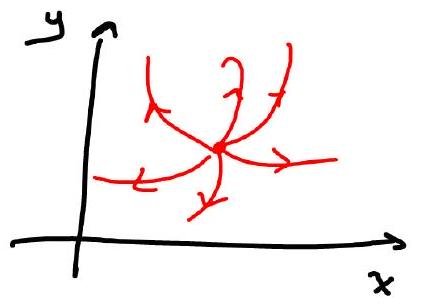
\includegraphics[width=0.5\textwidth]{2025_10_19_55a7d61d84e6ce9a1c8cg-4(2)}
\end{center}

$$
\lambda_{2}<\lambda_{1}<0
$$

stable node
\begin{center}
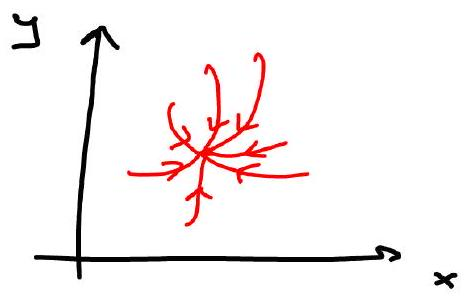
\includegraphics[width=0.5\textwidth]{2025_10_19_55a7d61d84e6ce9a1c8cg-4}
\end{center}

$$
\lambda_{2}<0<\lambda_{1}
$$

soddle node
\begin{center}
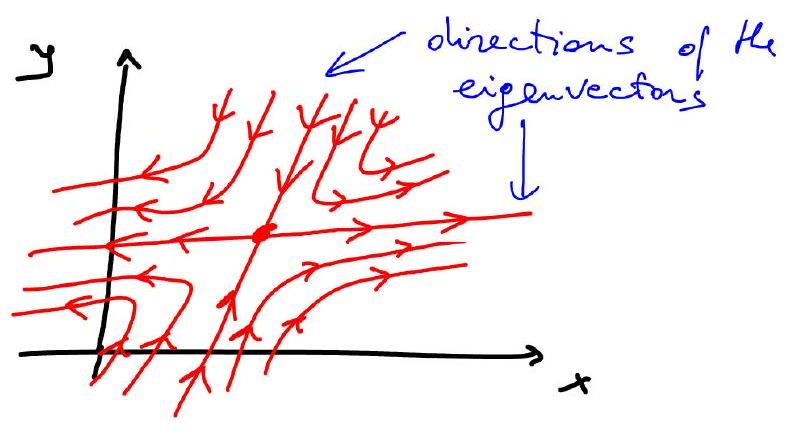
\includegraphics[width=0.5\textwidth]{2025_10_19_55a7d61d84e6ce9a1c8cg-4(3)}
\end{center}
$0<\lambda_{1}=\lambda_{2} \quad$ unstable stor

$$
\left(A=\lambda_{1} \|\right)
$$

\begin{center}
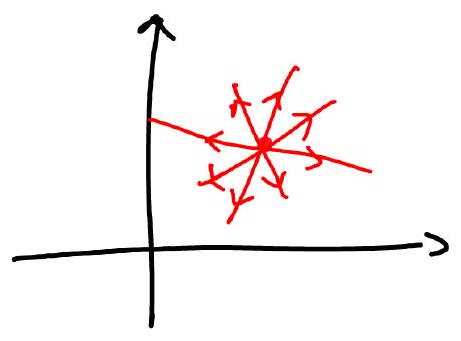
\includegraphics[width=0.5\textwidth]{2025_10_19_55a7d61d84e6ce9a1c8cg-4(1)}
\end{center}

$$
\begin{aligned}
& \lambda_{2}=\lambda_{1}<0 \quad \text { stoble stor } \\& (A=\lambda, 1)
\end{aligned}
$$

\begin{center}
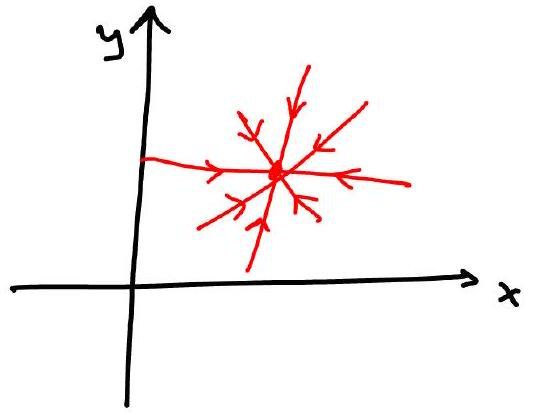
\includegraphics[width=0.5\textwidth]{2025_10_19_55a7d61d84e6ce9a1c8cg-5(1)}
\end{center}

If $A \neq \lambda_{1} \|$, then one gets degenerate (m)stable modes.
Complex eigenvolves

$$
\lambda_{1,2}=\gamma \pm i \omega
$$

$\\gamma<0 \quad$ stable focus

\begin{center}
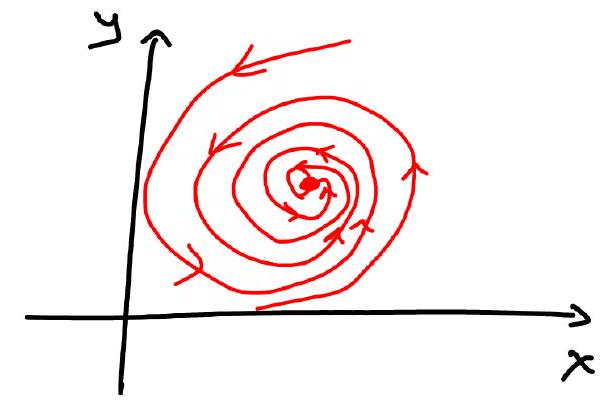
\includegraphics[width=0.5\textwidth]{2025_10_19_55a7d61d84e6ce9a1c8cg-5(3)}
\end{center}
\begin{center}
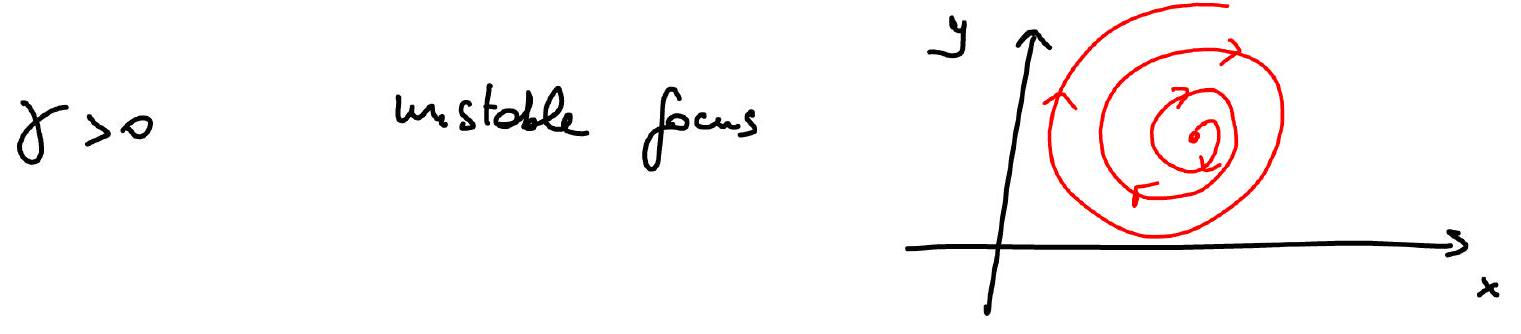
\includegraphics[width=0.5\textwidth]{2025_10_19_55a7d61d84e6ce9a1c8cg-5(4)}
\end{center}

All the above fixed points are hyperbalic. Here are a few examples of non-hyperbalic fixed points:

$$
\begin{array}{lll}
\lambda_{1}=0 & \lambda_{2}>0 & \text { line of } \\
& \left(\lambda_{1}<0\right) & \text { fixed point }
\end{array}
$$

\begin{center}
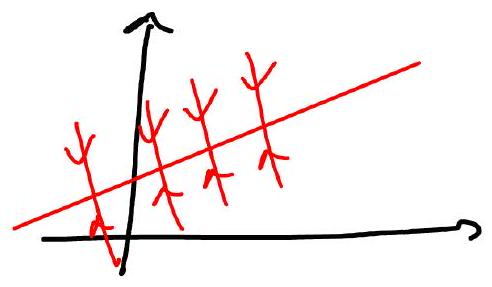
\includegraphics[width=0.5\textwidth]{2025_10_19_55a7d61d84e6ce9a1c8cg-5}
\end{center}

$$
\gamma=0 \quad \lambda_{2}= \pm i \omega
$$

\section*{center}
\begin{center}
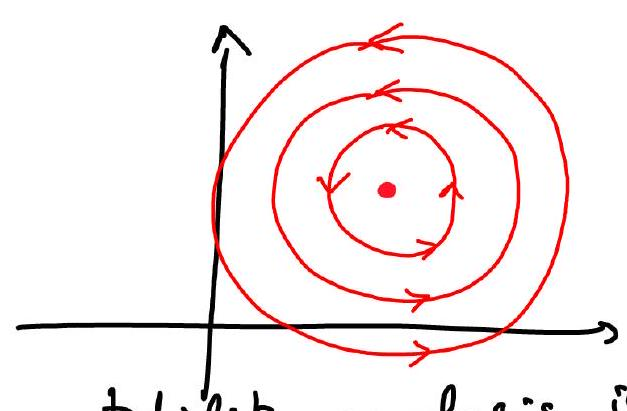
\includegraphics[width=0.5\textwidth]{2025_10_19_55a7d61d84e6ce9a1c8cg-5(2)}
\end{center}

On these latter cases the linear stobility anlysis is not sufficient to determine whether a fixed point is stable or not.

\section*{Exerciges}
\begin{enumerate}
  	item Find the fixed points of $\left\{\begin{array}{l}\\dot{x}=-x+x^{3} \\ \dot{y}=-2 y\end{array}\right.$ and classify them.
  	item Show that the linearization of the system
\end{enumerate}

$$
\left\{\begin{array}{l}
\dot{x}=-y+a x\left(x^{2}+y^{2}\right) \\dot{y}=x+a y\left(x^{2}+y^{2}\right)
\end{array}\right.
$$

incorrectly predicts that the origin is a center for all values of $a$. Indeed, the origin is a stable spinal if $a<0$, and unstable pinal if $a>0$.
[hint: to analize the nomlineer system, use polor coord. $x=r \cos \theta, y=r \sin \theta$ and find the equations for $r$ and $\theta$. Then interpret the non-lim. System.]
3) The equation of motion of a porticle is $\\ddot{x}=x-x^{3}$. Find the fixed points and classify flem. Show that the function $E=\\frac{\\dot{x}^{2}}{2}-\\frac{x^{2}}{2}+\\frac{x^{4}}{4}$ (the energy) is conserved by the dynamics and that the trajectories are clased curves difined by the contours of $E$. Draw the phase pertrait.
4) Study the system of $O D E S$ :

$$
\begin{array}{ll}
\dot{x}=x(3-x-2 y) & x, y \geqslant 0 \\dot{y}=y(2-x-y) &
\end{array}
$$

Find the fixed points and classify them. Show that the phose portroit is
\begin{center}
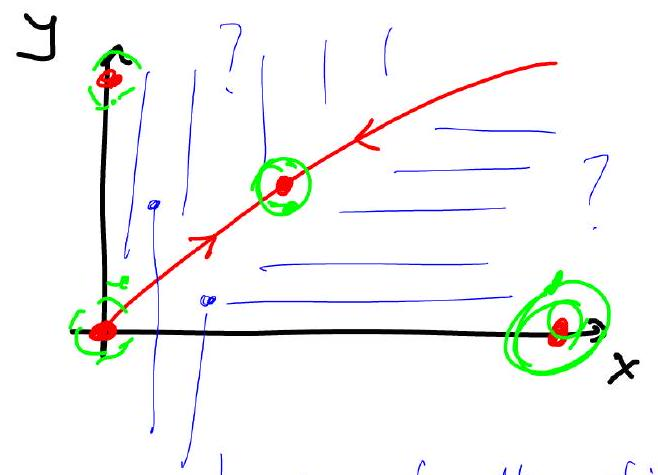
\includegraphics[width=0.5\textwidth]{2025_10_19_55a7d61d84e6ce9a1c8cg-7}
\end{center}
\basin of attraction: the set of all initial conditions which end up in one fixed point as $t \rightarrow \infty$ )

\section*{PROPERTIES OF DIFFUSION}
A first simple derivation
Let us consider a larg and thin tube filled with weter. At time $t=0$ we inject a unit amount of ink at $x=0$

Brownion mostion of pentides

$$
\begin{gathered}
 t=0, x=0 \quad V(x, t)=\text { sumal } \\W(x, t)=\frac{\# \text { of porticles in } V(x, t)}{V(x, t)}
\end{gathered}
$$
$W(x, t)$ is the density of "ink" (or Brownion) particles at position $x \in \mathbb{R}$, time $t \geqslant 0$ as the valume $V \rightarrow 0$ and the number of particle $ightarrow \infty$.
$\\int_{A} W(x, t) d x:=\text { prob. to find a porticle in the rigion } A \subseteq \mathbb{R}$. assuming that $\\int_{-\infty}^{+\infty} w(x, t) d x=1$.
% Lecture file created by newnote
% Class: Models of Theoretical Physics
% Professor: Azaele Sandro
% Date: 2025-10-10
\lecture{15}{Laplace method continued}{2025-10-10}
\pagelayout{margin}
% --- Start writing here ---

\section{Laplace method continued}
\subsection*{The Laplace method}
In several situations we wish to evaluate complicated integrals which have a form
\begin{DispWithArrows}[tag=21]
    I(\lambda)=\int_{x_{1}}^{x_{2}} d x g(x) e^{\lambda f(x)} \quad \lambda \in \mathbb{R}
\end{DispWithArrows}
where $g$ and $f$ are continuous and differentiable functions. Although $I(\lambda)$ cannot be calculated for any arbitrary $\lambda$, it happens that it can be well approximated (under appropriate conditions) as $\lambda \rightarrow \infty$.
The core idea of Laplace's method is that the major contribution to the integral in (21) as $\lambda \rightarrow \infty$ comes from the neighborhood of the point in $\left[x_{1}, x_{2}\right]$ where $f(x)$ gets its maximum value, which we call $x_{0}$.
\begin{figure}[H]
    \centering
    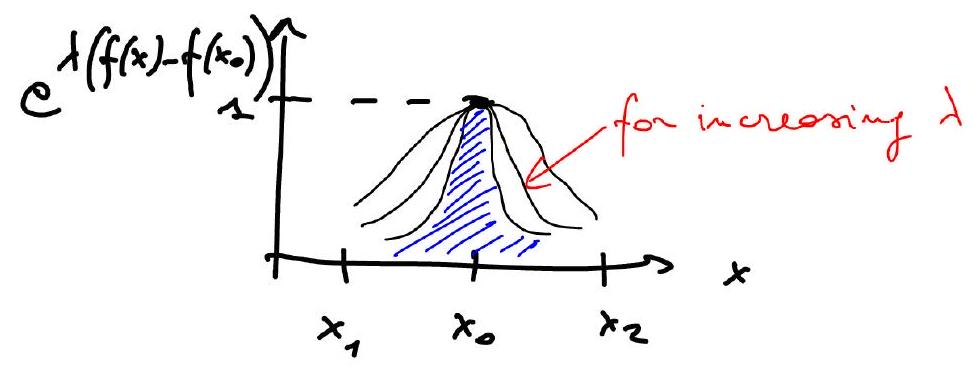
\includegraphics[width=\textwidth]{2025_10_19_6d9f59a2c3b97d481c52g-1}
\end{figure}
There are essentially three cases:
\begin{enumerate}
    \item $x_{0}$ is an interior maximum, $x_{1}<x_{0}<x_{2}$ and $f^{\prime}\left(x_{0}\right)=0$. We assume that $f^{\prime \prime}\left(x_{0}\right)<0$ (actually if $f^{\prime}\left(x_{0}\right)=f^{\prime \prime}\left(x_{0}\right)=f^{\prime \prime \prime}\left(x_{0}\right)=0$ but $f^{(iv)}\left(x_{0}\right)<0$ we can apply very similar ideas and the calculations are not more difficult). Also $g\left(x_{0}\right) \neq 0$ and it is finite.
\end{enumerate}
As we expect that the dominant contributions comes from the neighborhood of $x_{0}$ and $f(x)=f\left(x_{0}\right)+\frac{\left(x-x_{0}\right)^{2}}{2} f^{\prime \prime}\left(x_{0}\right) +O\left(\left|x-x_{0}\right|^{3}\right)$ as $x \rightarrow x_{0}$, we obtain
\begin{DispWithArrows}
    I(\lambda) \cong \int_{x_{1}}^{x_{2}} g(x) e^{\lambda\left(f\left(x_{0}\right)+\frac{\left(x-x_{0}\right)^{2}}{2} f^{\prime \prime}\left(x_{0}\right)\right)} d x \simeq g\left(x_{0}\right) e^{\lambda f\left(x_{0}\right)} \int_{x_{1}}^{x_{2}} e^{-\lambda \frac{\left|f^{\prime \prime}\left(x_{0}\right)\right|}{2}\left(x-x_{0}\right)^{2}} d x
\end{DispWithArrows}
We change var. $s=\left(x-x_{0}\right) \sqrt{\frac{\left|f^{\prime \prime}\left(x_{0}\right)\right|}{2} \lambda}$ so
\begin{DispWithArrows}
    I(\lambda) \simeq g\left(x_{0}\right) e^{\lambda f\left(x_{0}\right)} \sqrt{\frac{2}{\lambda\left|f^{\prime \prime}\left(x_{0}\right)\right|}} \int_{\left(x_{1}-x_{0}\right) \sqrt{\frac{\left|f^{\prime \prime}\left(x_{0}\right)\right| \lambda}{2}}}^{\left(x_{2}-x_{0}\right) \sqrt{\frac{\left|f^{\prime \prime}\left(x_{0}\right)\right| \lambda}{2}}} e^{-s^{2}} d s
\end{DispWithArrows}
as $\lambda \rightarrow \infty \rightarrow \int_{-\infty}^{+\infty} e^{-s^{2}} d s=\sqrt{\pi}$
\begin{DispWithArrows}[tag=22]
    I(\lambda) \simeq g\left(x_{0}\right) e^{\lambda f\left(x_{0}\right)} \sqrt{\frac{2 \pi}{\lambda\left|f^{\prime \prime}\left(x_{0}\right)\right|}} \quad \text { as } \lambda \rightarrow+\infty \text { (leading order)}
\end{DispWithArrows}
one should prove that this is the leading order (we did not).

Exercise: show that the next to leading order of $I(\lambda)$ in eq. (22) is given by
\begin{DispWithArrows}
    I(\lambda)=e^{\lambda f\left(x_{0}\right)} \sqrt{\frac{2 \pi}{\lambda\left|f^{\prime \prime}\left(x_{0}\right)\right|}}\left(g\left(x_{0}\right)+\frac{c}{\lambda}\right) \quad \text { as } \lambda \rightarrow \infty
\end{DispWithArrows}
where $c$ is a constant that depends on the derivatives of $f$ up to $4^{\text {th }}$ order (at $x=x_{0}$) and on $g\left(x_{0}\right)$ and $g^{\prime}\left(x_{0}\right)$.
\begin{enumerate}
    \setcounter{enumi}{1}
    \item $x_{0}=x_{1}$ or $x_{0}=x_{2}$ ($x_{0}$ is a flat endpoint) and $f^{\prime}\left(x_{0}\right)=0$.
    \begin{figure}[H]
        \centering
        \includegraphics[width=0.5\textwidth]{2025_10_19_6d9f59a2c3b97d481c52g-3}
    \end{figure}
    It is easy to show that the leading order formula is
    \begin{DispWithArrows}[tag=23]
        I(\lambda) \simeq g\left(x_{0}\right) e^{\lambda f\left(x_{0}\right)} \sqrt{\frac{\pi}{2 \lambda\left|f^{\prime \prime}\left(x_{0}\right)\right|}}
    \end{DispWithArrows}
\end{enumerate}
\subsection*{Example}
The modified Bessel function of second kind is a special function that occurs in many applications. It is given by
\begin{DispWithArrows}
    K_{\nu}(x)=\int_{0}^{\infty} e^{-x \cosh t} \cosh (\nu t) d t, x>0
\end{DispWithArrows}
we wish to estimate $K_{\nu}(x)$ as $x \rightarrow+\infty$ for fixed $\nu$. Since $\cosh^{\prime}(t)=\sinh (t)>0$ for $t>0$, the max of $e^{-x \cosh t}$ as a function of $t(x>0)$ occurs at $t=0$, with zero derivative.

So we can apply eq. (23) ($\cosh t \simeq 1+\frac{t^{2}}{2}+\cdots$) $f(t)=-\cosh t$
\begin{DispWithArrows}
    K_{\nu}(x) \simeq e^{-x} \sqrt{\frac{\pi}{2x}}
\end{DispWithArrows}
as $x \rightarrow \infty$ at leading order.

Notice that it does not depend on $\nu$!
Exercise: show that
\begin{DispWithArrows}
    K_{\nu}(x)=\sqrt{\frac{\pi}{2x}} e^{-x}\left(1+\frac{c(\nu)}{x}+\cdots\right)
\end{DispWithArrows}
and $c(\nu)=\frac{4 \nu^{2}-1}{8}$.
\begin{enumerate}
    \setcounter{enumi}{2}
    \item $x_{0}=x_{1}$ or $x_{0}=x_{2}$ ($x_{0}$ is an endpoint) but $f^{\prime}\left(x_{0}\right) \neq 0$. Without loss of generality we take $x_{0}=x_{1}$ and $f^{\prime}\left(x_{0}\right)<0$.
    \begin{figure}[H]
        \centering
        \includegraphics[width=0.5\textwidth]{2025_10_19_6d9f59a2c3b97d481c52g-4}
    \end{figure}
    In this case we get $f(x)=f\left(x_{0}\right)+\left(x-x_{0}\right) f^{\prime}\left(x_{0}\right)+\cdots$
    hence
    \begin{DispWithArrows}
        \begin{aligned}
        I(\lambda) & \cong \int_{x_{1}=x_{0}}^{x_{2}} g(x) e^{\lambda\left[f\left(x_{0}\right)+\left(x-x_{0}\right) f^{\prime}\left(x_{0}\right)
ight]} d x \\
        & =g\left(x_{0}\right) e^{\lambda f\left(x_{0}\right)} \int_{x_{0}}^{x_{2}} e^{\lambda\left[\left(x-x_{0}\right) f^{\prime}\left(x_{0}\right)
ight]} d x \\
        & =g\left(x_{0}\right) e^{\lambda f\left(x_{0}\right)} \int_{0}^{x_{2}-x_{0}} e^{\lambda f^{\prime}\left(x_{0}\right) s} d s=\frac{g\left(x_{0}\right) e^{\lambda f\left(x_{0}\right)}}{\lambda f^{\prime}\left(x_{0}\right)}\left[e^{\lambda s f^{\prime}\left(x_{0}\right)}
ight]_{0}^{x_{2}-x_{1}}
        \end{aligned}
    \end{DispWithArrows}
as $\lambda \rightarrow \infty$ and $f^{\prime}\left(x_{0}\right)<0$ we get
    \begin{DispWithArrows}[tag=24]
        I(\lambda) \cong g\left(x_{1}\right) \frac{e^{\lambda f\left(x_{1}\right)}}{\lambda\left|f^{\prime}\left(x_{1}\right)\right|} \quad \text { as } \lambda \rightarrow \infty
    \end{DispWithArrows}
\end{enumerate}
\subsection*{Example:}
Obtain the leading order approximation of
\begin{DispWithArrows}
    I(\lambda)=\int_{0}^{1} x^{m} e^{\lambda\[3 x^{2}+2 x^{3}\]} d x \quad \text { as } \lambda \rightarrow+\infty
\end{DispWithArrows}
\begin{figure}[H]
    \centering
    \includegraphics[width=0.5\textwidth]{2025_10_19_6d9f59a2c3b97d481c52g-5}
\end{figure}
The max is at $x=1, f(1)=5, f^{\prime}(1)=12, g(1)=1$. We can apply eq. (24)
\begin{DispWithArrows}
    I(\lambda) \simeq \frac{e^{5\lambda}}{12 \lambda}
\end{DispWithArrows}
\subsection*{Exercise:}
Calculate the leading order approx. when the integral is
\begin{DispWithArrows}
    \int_{-1}^{0} \cdots=? \quad \int_{-2}^{0} \cdots=?
\end{DispWithArrows}
\subsection*{Stirling formula}
We want to estimate how fast $N!$ goes to infinity as $N \rightarrow \infty$. We will apply the Laplace's method to the gamma function:
\begin{DispWithArrows}[tag=25]
    \Gamma(\lambda)=\int_{0}^{\infty} x^{\lambda-1} e^{-x} d x \quad \lambda>0
\end{DispWithArrows}
Exercise: Show that $\Gamma(\lambda+1)=\lambda \Gamma(\lambda)$ hence $\lambda!=\Gamma(\lambda+1)$ which generalize the factorial to complex numbers.

Let's consider $\Gamma(\lambda+1)=\int_{0}^{\infty} x^{\lambda} e^{-x} d x$. If we write this as $\int_{0}^{\infty} e^{-x} e^{\lambda \ln x} d x$ we cannot apply Laplace's method. It is more beneficial to consider the max of the function $f(x)=-x+\lambda \ln x$ and set $g(x)=1$. The max occurs at $x=\lambda$ which suggests a change of var: $x=\lambda t$ (so the max is now fixed w.r.t. t). We get
\begin{DispWithArrows}
    \Gamma(\lambda+1)=\int_{0}^{\infty} x^{\lambda} e^{-x} d x=\lambda^{\lambda+1} \int_{0}^{\infty} t^{\lambda} e^{-\lambda t} d t
\end{DispWithArrows}
$t^{\lambda} e^{-\lambda t}=e^{\lambda(\ln t-t)} \quad h(t)=\ln t-t, \quad h^{\prime}(1)=0, h^{\prime \prime}(1)=-1$. In this way we can apply eq. (22) with $g(t)=1 \quad\left(t_{0}=1\right)$.
\begin{DispWithArrows}[tag=26]
    \Gamma(\lambda+1)=\lambda!\simeq \lambda^{\lambda+1} e^{-\lambda} \sqrt{\frac{2 \pi}{\lambda}} \quad \text { as } \lambda \rightarrow \infty
\end{DispWithArrows}
Exercise: Show that at leading order
\begin{DispWithArrows}
    \int_{0}^{\infty} e^{-\lambda t} e^{-\frac{1}{t}} d t \cong \frac{\sqrt{\pi} e^{-2 \sqrt{\lambda}}}{\lambda^{3 / 4}} \quad \text { as } \lambda \rightarrow \infty
\end{DispWithArrows}
\subsection*{Example:}
Let's consider the class of integrals:
\begin{DispWithArrows}
    I_{m}(x)=\int_{0}^{\infty} t^{m} e^{-\frac{t^{2}}{2}-\frac{x}{t}} d t \quad x>0 .
\end{DispWithArrows}
We calculate $I_m(x)$ for large $x$ and fixed m.
$rac{t^{2}}{2}+rac{x}{t}$ has a movable min at $rac{d}{d t}
\left(rac{t^{2}}{2}+\frac{x}{t}\right)=0, \bar{t}=x^{1 / 3}$. So we introduce the new variable $\tau$:
\begin{DispWithArrows}
    t=x^{1 / 3} \tau
\end{DispWithArrows}
So
\begin{DispWithArrows}
    I_{m}(x)=x^{\frac{m+1}{3}} \int_{0}^{\infty} \tau^{m} e^{-x^{2 / 3}\left(\frac{\tau^{2}}{2}+\frac{1}{\tau}\right)} d \tau
\end{DispWithArrows}
The min of the exponent occurs at $\tau=1$ (interior) so we can apply eq. (22):
\begin{DispWithArrows}
    \begin{aligned}
    I_{m}(x) & =x^{\frac{m+1}{3}} e^{-\frac{3}{2} x^{2 / 3}} \sqrt{\frac{2 \pi}{x^{2 / 3} \cdot 3}} \\ &=x^{m / 3} e^{-\frac{3}{2} x^{2 / 3}} \sqrt{\frac{2 \pi}{3}}
    \end{aligned}
\end{DispWithArrows}
as $x \rightarrow \infty$. leading order, fixed $m$

\subsection*{Exercises:}
\begin{DispWithArrows}
    \begin{aligned}
    & \int_{-2}^{0} e^{t} e^{\lambda\[3 t^{2}+2 t^{3}\]} d t \simeq e^{\lambda-1} \sqrt{\frac{\pi}{3 \lambda}} \\
    & \int_{0}^{1} e^{t} e^{\lambda\[3 t^{2}+2 t^{3}\]} d t \simeq \frac{e^{5\lambda+1}}{12 \lambda} \\
    & \int_{0}^{1} \sqrt{1+t} e^{\lambda\[2 t-t^{2}\]} d t \simeq e^{\lambda} \sqrt{\frac{\pi}{2 \lambda}} \\
    & \int_{-1}^{2} e^{\lambda\[t^{3}-1\]}\left(1+t^{2}\right) d t \simeq \frac{5 e^{7\lambda}}{11 \lambda}
    \end{aligned}
\end{DispWithArrows}
Question: Let's assume that $f(x)$ behaves like in the fig:
\begin{figure}[H]
    \centering
    \includegraphics[width=0.5\textwidth]{2025_10_19_6d9f59a2c3b97d481c52g-8}
\end{figure}
Where does the leading order come from?



\backmatter
% Bibliography, index, etc.
\printbibliography

\end{document}
